
\section{Comparison of \beetle{} and L2LMs}\label{sec:lit-review}


\begin{figure}[t!]
    \centering
    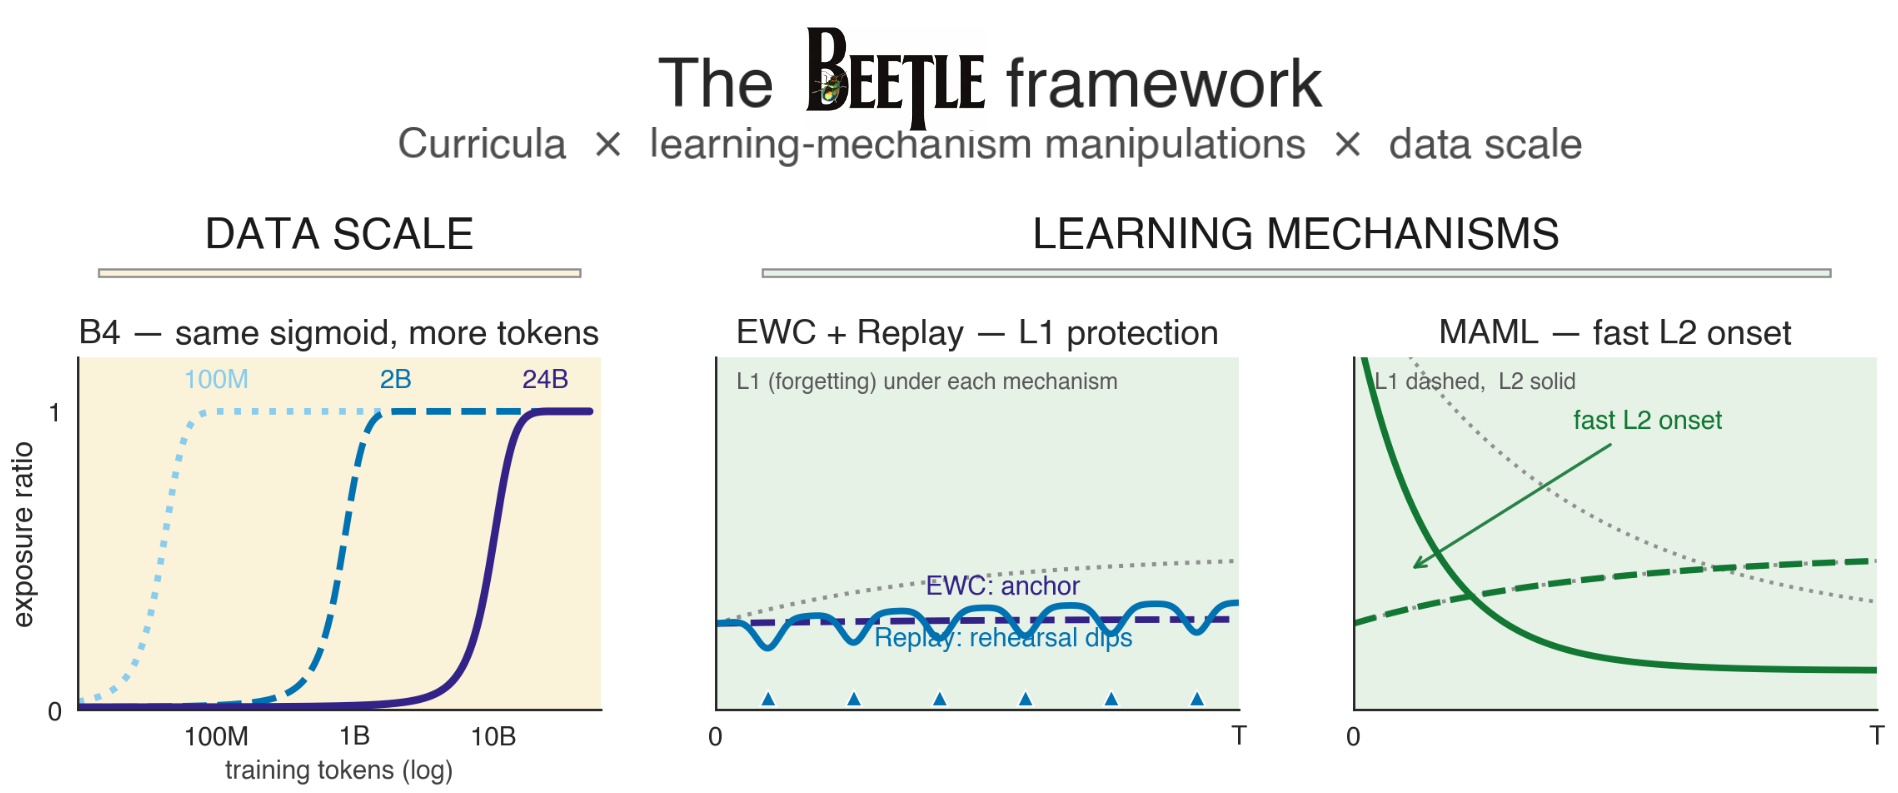
\includegraphics[width=0.85\linewidth]{fig/logo/3.png}
    \caption{Schematic comparison of the five \beetle{} bilingual exposure curricula B1--B5 (cf.\ Tab.~\ref{tab:curricula-overview}); the L1:L2 token-mix trajectory across training is rendered for each curriculum, with B2/B3/B5 sharing a sigmoid L2-onset and B4 a constant-mean-with-bursts schedule from step~0.}
    \label{fig:beetle}
\end{figure}


\begin{table}[!ht]
        \begin{tabular}{lccccc c}
        \toprule
        \textbf{Work} & \textbf{S} & \textbf{CL} & \textbf{M} & \textbf{C} & \textbf{CF} & \textbf{Dim} \\
        \midrule
        Constantinescu et al.\ (2025) & W & -- & -- & EWC & -- & $\triangle$ \\
        Arnett et al.\ (2025)         & W & -- & \checkmark & -- & -- & $\triangle\triangle$ \\
        Aoyama et al.\ (2024)         & W & -- & -- & -- & RT & $\triangle$ \\
        Diehl Martinez et al.\ (2025) & W & -- & -- & -- & -- & $\triangle\triangle$ \\
        Anon.\ (2025)                 & H & \checkmark & \checkmark & -- & -- & $\triangle\triangle\triangle$ \\
        Diehl Martinez et al.\ (2023) & H & \checkmark & -- & -- & -- & $\triangle\triangle\triangle$ \\
        Mita et al.\ (2025)           & H & -- & -- & -- & WM & $\triangle\triangle$ \\
        \midrule
        \textbf{BeetleLM}
        & \textbf{H+W}
        & \checkmark
        & \checkmark
        & \checkmark
        & \checkmark
        & $\triangle\times7$ \\
        \bottomrule
        \end{tabular}
\end{table}

Bilingual and second-language language models (L2LMs) have been explored through a range of architectural and training regimes aimed at simulating second language acquisition, while increasingly serving as testbeds for cognitively grounded evaluation via surprisal-based reading-time prediction. Early computational approaches framed SLA as sequential adaptation in probabilistic or neural models \citep{matusevych-etal-2013-computational}, while more recent work has formalised bilingual training as controlled pretraining or adaptation processes in large language models. For example, \citet{aoyama2024modeling} propose a two-phase regime in which a model is first trained on L1 data and then adapted to L2 while freezing most parameters except embeddings and the LM head, showing that constrained plasticity can preserve prior knowledge while enabling new-language acquisition. \citet{constantinescu2025investigating} extend this direction by systematically varying exposure schedules and loss functions, including Elastic Weight Consolidation, to study trade-offs between stability and plasticity under continual bilingual training. More recently, \citet{arnett-etal-2025-acquisition} introduce B-GPT and contrast sequential versus simultaneous bilingual pretraining, finding that mixed exposure better approximates naturalistic bilingual learning dynamics, while \citet{feng2026bilingual} study scaling effects in bilingual machine translation settings and show that data composition and scale strongly influence cross-lingual transfer, albeit with primarily task-based evaluation. Earlier multilingual CDS-style L2LMs \citep{yadavalli-etal-2023-slabert, oba-etal-2023-second} explore similar ideas but are limited in language coverage, checkpointing, and evaluation depth. 

A key motivation for these models is their use as cognitive proxies through surprisal-based reading-time prediction, where processing difficulty is linked to a word’s unexpectedness under a language model, formalised as $-\log P(w_i \mid w_{<i})$. This framework underlies psycholinguistic models of reading time and is typically operationalised via regression models that combine surprisal with lexical covariates, often evaluated through changes in log-likelihood ($\Delta$LL) between baseline and surprisal-augmented models \citep{wilcox2020predictive, kaye2025sentence}. However, psychometric predictive power (PPP) is not a simple function of model quality, reflecting instead how well model probabilities align with human processing distributions \citep{de-varda-marelli-2022-effects, goodkind-bicknell, demberg-keller, shain2019, shain2021, hoover2022}. Despite extensive work in L1 psycholinguistics, there remains comparatively limited work on L2 cognitive modelling with language models, even though L2 reading is known to exhibit systematic cross-linguistic variation and proficiency effects \citep{hillert1998sentence, meister2021revisiting, kuribayashi-etal-2021-lower} and has been studied experimentally in psycholinguistics (Cop et al., 2015; Grüter et al., 2014, 2017; Kaan et al., 2010; Martin et al., 2013). 

Against this backdrop, \textsc{Beetle} extends prior L2LM work in three key ways: it specifies eight typologically diverse L1s for this paper (three released bilingually at FineWeb, five corpus-prepared; framework pool 38), parameterises exposure along six continuous dimensions rather than binary sequential/simultaneous splits, and integrates cognitively and pedagogically grounded evaluations including MECO L2 reading times, BLiSS, and CEFR proficiency measures. Its continual-learning framework unifies prior isolated strategies, with EWC, MAML-style adaptation, and learning-rate plasticity subsuming earlier single-method approaches such as those in \citet{constantinescu2025investigating}, while embedding-and-LM-head-only adaptation corresponds to a special case within its broader set of 15 training regimes. Finally, unlike prior work focused on limited bilingual corpora or synthetic MT settings, \textsc{Beetle} evaluates models trained on large-scale real web data (FineWeb) across 100M, 2B, and 24B token regimes, directly linking scaling, cross-lingual transfer, and psycholinguistic predictive power within a unified evaluation framework.


 \textsc{Beetle}'s EWC, MAML and LR-plasticity controls subsume the single-strategy approaches of \citet{constantinescu2025investigating}; \citet{aoyama2024modeling}'s embedding-and-LM-head-only adaptation is one preset within \textsc{Beetle}'s 15 continual-learning strategies. \citet{feng2026bilingual} match mono- and bi-lingual 100M LMs on synthetic MT data; \textsc{Beetle} matches them on real FineWeb at 100M, 2B and 24B with psycholinguistic and pedagogical readouts. Earlier multilingual CDS L2 LMs \citep{yadavalli-etal-2023-slabert, oba-etal-2023-second} cover fewer languages, lack checkpointing, and use only grammaticality readouts.


 Surprisal efforts can be interpreted as cognitive costs associated to a shift between probabilistic distributions \citep{de-varda-marelli-2022-effects}. Surprisal Theory (Hale, Levy), which quantifies how unpredictable a word is in terms of negative logarithm of word conditioned by previous sentential context, is a linking function between measured cognitive effort and predicability (measured as the Kullback-Leibler divergence/relative entropy between distributions).   \[\text{surprisal}(w_i) = - log_2 P(w_i |w_1, w,2, \dots, w_{i-1})\] The \textbf{Psychometric Predictive Power (PPP)} of a LM is \textit{not} a linear function of model quality (\textit{pace} \citet{de-varda-marelli-2022-effects}, also Goodkind and Bicknell; Demberg and Keller, Shain 2019, 2021; Hoover et al 2022).  However, multiple sentence processing has significant cross-linguistic variation \cite{hillert1998sentence} Dutch \cite{meister2021revisiting}, Japanese \citep{kuribayashi-etal-2021-lower} Although the vast majority of studies focus on L1, there is increasing interest in L2 predictive processing – (Cop et al., 2015; Grüter et al., 2014, 2017; Kaan et al., 2010; Martin et al., 2013).  Following prior work \citep{wilcox2020predictive, kaye2025sentence}, we measure predictive power for data point $i$ using the change in log-likelihood:
 \begin{equation}
 \Delta \mathrm{LL}_i =
 \log L_{\text{target}}(RT_i \mid x_{\text{target}})
 -
 \log L_{\text{baseline}}(RT_i \mid x_{\text{baseline}})
 \end{equation}

 where $RT_i$ is the reading-time measure of a single participant on a given word, $x_{\text{baseline}}$ are the control predictors, and $x_{\text{target}}$ are the target predictors, which include the control predictors together with surprisal.\footnote{Baseline model formula in \texttt{R}:
 \texttt{RT $\sim$ te(freq, len) + te(freq\_prev, len\_prev)}}\footnote{Linear surprisal model formula in \texttt{R}:
 \texttt{RT $\sim$ surp + surp\_prev + te(freq, len) + te(freq\_prev, len\_prev)}}\footnote{Non-linear surprisal model formula in \texttt{R}:
 \texttt{RT $\sim$ s(surp, k = 6) + s(surp\_prev, k = 6) + te(freq, len) + te(freq\_prev, len\_prev)}. The value of $k$ follows prior work \citep{wilcox2023}.}

\paragraph{Learning dynamics, cognates, BLiSS.} \citet{aoyama-wilcox-2025-language} place the monolingual PPP tipping point at $\sim$2B tokens; we test whether structured-exposure curricula can delay or eliminate this decay in bilingual training. \citet{aoyama2025predicting} show induction-head emergence is data-property-driven; we quantify how exposure curriculum shifts emergence timing across L1 and L2. \citet{frank2026dutch} report Dutch--English cognate / false-friend effects which we connect to MECO L2 reading. The BLiSS task / dataset is due to \citet{gao2025bliss}: a CEFR-stratified discrimination of artificial vs.\ learner errors. We adopt their NGS / CPS / RP$@\tau$ protocol unchanged and sweep across our curriculum grid.

paragraph{Pedagogical CEFR simulation and cognitive constraints.} \citet{benedetto-etal-2024-using} score frontier LMs (GPT-3.5 / GPT-4) on the CUP\&A5 dataset \citep{mullooly2023cupa5} (200 MCQA $\times$ 4 CEFR levels) using the metric $M = \rho_{L,I} - P$, with $\rho_{L,I}$ the Spearman rank correlation between simulated CEFR-level accuracy and item difficulty and $P$ a penalty for non-monotonic learner curves. They simulate CEFR via prompt engineering; Beetle simulates CEFR via training-time exposure curricula and identifies the best Beetle checkpoint that yields a CEFR-monotonic accuracy curve. Cognitive-constraint priors --- Shuffle-Dyck pre-pretraining \citep{hu2025between} and ALiBi-decay working memory \citep{mita2025wm, madhayastha2026wm} --- are implemented as opt-in modules in Beetle's architecture registry rather than headline contributions.


paragraph{Phase Transition in Language Model Pretraining and PPP } \textbf{Phase Transitions } in LM pretraining refer to abrupt behavioural changes \citep{oh2023does, michaelov2025language, chang2025bigram, nakagi2025triple}.  The abrupt emergence of specialised \textbf{induction heads} \citep{chensudden, aoyama2025predicting}. Empirically, induction heads form early in training (as long as models have multiple heads and at least two layers).  Mathematically, it is equivalent to a type of Bayesian inference. \citet{aoyama-wilcox-2025-language} find 


%\textbf{2B Pretraining Hypothesis \citep{oh2023transformer}} 



%\paragraph{Modelling Human Language Processing}  Language model surprisal has been shown to be a strong predictor of metrics of online human language processing, e.g. predicting the time it takes to read a word \cite{kuribayashi-etal-2021-lower}. Larger Transformer-based language models and models trained on more data have been found to be worse at modelling human reading behaviour \citep{oh2023transformer, wilcox2025bigger, michaelov2025language, michaelov2026n}.  Recent work by \citet{aoyama-wilcox-2025-language} has shown that past 2 billion tokens of monolingual pretraining, model psychometric predictive power (PPP) begins to decrease. %identified a \textit{tipping point in model psychometric predictive power (PPP)} at 2 billion tokens in monolingual pretraining. %Minimal pair evaluation datasets  – such as BLiMP \citep{warstadt-etal-2020-blimp-benchmark}, MultiBLiMP \citep{jumelet2025multiblimp}, and language-specific BLiMP variants (e.g., BLiMP-NL for Dutch and Zho-BLiMP for Chinese) – are also used to evaluate the syntactic competence of a language model compared to a native (L1) fluent speaker. 

%



%\paragraph{Human-Scale Language Modelling} The BabyLM challenge encourages development of sample-efficient, human-scale language models, trained on just 100M words \citep{warstadt2023findings, warstadt2024insights, hu2024findings, charpentier2025findings, choshen2026babylm}. While the majority of such \ efforts have focused on English, the curation of human-scale training data beyond English, e.g. \citet{jumelet2025babybabellmmultilingualbenchmarkdevelopmentally},  has facilitated the training of monolingual language models beyond English  \citep{salhan-etal-2024-less, prevot-etal-2024-extending, matzopoulos-etal-2025-babylms, capone-etal-2024-babies, padovani-etal-2025-child, shen-etal-2024-bambino, goriely-buttery-2025-ipa}. 

%\paragraph{Bilingual and Second-Language Language Models (L2LMs)}  L2LMs (coined in \citet{aoyama2024modeling}) are bilingual language models trained sequentially on two languages that are computational cognitive models of second language acquisition (SLA) \citep{matusevych-etal-2013-computational}.  \citet{aoyama2024modeling} use a two-phase method in which models are first trained on L1 only. In the second phase, all model weights except for the embeddings and LM head are frozen, and the model is trained on data from L2.  \citet{constantinescu2025investigating} use two different training approaches: exposure scheduling and modified loss function. They use Elastic Weight Consolidation as a way of enforcing plasticity. However, there is significant variation in the quantity and nature of L2LM training data and training architecture. Recently, \citet{arnett-etal-2025-acquisition} introduce B-GPT (Bilingual GPT) which contrasts a \texttt{sequential} bilingual regime (similar to standard L2LM pretraining) with a \texttt{simultaneous} regime (more similar to later L2 acquisition with mixed L1 and L2 exposure). 

%There have been different approaches to training bilingual models for the purpose of studying second-language acquisition. 
% There are broadly three types approaches that draw on a Bilingual Language Model paradigm in multilingual NLP:

%\paragraph{Catastrophic Forgetting and Continual Learning} It has been widely observed that continual pretraining, curriculum learning, or domain adaptation can lead to catastrophic forgetting, resulting in degradation on tasks or languages that are otherwise not present in finetuning data. In multilingual continual pretraining contexts, this results in a loss of capability in languages that they were not fine-tuned on \citep{vu-etal-2022-domain, sun-etal-2023-efficiently, winata-etal-2023-overcoming, alexandrov-etal-2024-mitigating, liu-niehues-2025-conditions}. The adaptation of monolingual LLMs requires adequate consideration of catastrophic forgetting and tokenizer limitations. Successful strategies utilise a combination of (i) vocabulary extension according to an optimal extension ratio and (ii) embedding alignment. In case of bilingual pretraining, recent work has identified a \textit{curse of bilinguality} \citep{zhou-matusevych-2025-curse}. 

%\paragraph{Data Quality} Data Quality of large web-crawled data is an important confound of multilingual pretraining at scale. Cross-lingual data contamination (e.g., due to poor natural language identification in preprocessing) is an issue for investigating questions of cross-lingual transfer \citep{blevins-zettlemoyer-2022-language}.  \citet{seto-etal-2025-assessing} on bilingual data quality... 

% \subsection{Cognitive Modelling of Bilingual, Second and Polyglot Language Learning}

% \subsection{Bilingual Interpretability for Cross-Lingual Transfer}

% Bilingual interpretability offers a uniquely tractable and theoretically clean setting for understanding how language models internalize and transfer linguistic knowledge across languages \citep{inaba-etal-2025-bilingual}. Unlike massively multilingual models, where heterogeneous scripts, typologies, and resource imbalances confound analysis, bilingual models isolate cross-lingual phenomena to a controlled two-language system, making it possible to precisely track how syntax, semantics, morphology, and cultural knowledge are shared or segregated across representations. This simplicity enables fine-grained mechanistic analysis—at the level of neurons, attention heads, and latent subspaces—while still capturing the core challenges of cross-lingual generalization and transfer. 

% As a result, bilingual interpretability serves both as a methodological testbed for developing and validating interpretability tools and as a substantive scientific probe into the emergence of language-neutral representations, asymmetries in transfer, and the inductive biases that govern multilingual learning. Insights gained in the bilingual regime can then be systematically scaled to multilingual settings, grounding broader cross-lingual interpretability claims in a controlled and explainable foundation.

%\paragraph{Phase Transitions and Human-Likeness} Recent work by \citet{aoyama-wilcox-2025-language} has identified a \textit{tipping point in model psychometric preditive power (PPP)} at 2 billion tokens in monolingual pretraining. 



\section{\beetle{} Training Framework}\label{sec:train}

\beetle{} is built on a custom \textsc{Pico} decoder stack \citep{diehl-martinez-etal-2025-pico} with curriculum-aware checkpointing, a registry of fifteen continual-learning strategies, and a tokeniser layer that supports per-language, shared-bilingual, and shared-trilingual vocabularies. The composable schedule primitives that govern multilingual exposure (\textsc{ConstantExposure}, \textsc{SigmoidRamp}, \textsc{LinearRamp}, \textsc{BurstSchedule}, \textsc{CyclicalSchedule}, \textsc{CompositeSchedule}) and the optional \textsc{EpisodicSampler} that groups consecutive batches into named contexts (\emph{home} vs.\ \emph{classroom}, etc.) implement the full enumeration described in the body. Ten predefined acquisition conditions in \texttt{condition\_presets.py} map psycholinguistic scenarios to concrete schedule parameters.

\subsection{Architecture Registry}\label{sec:beetle-architecture-registry}

The body backbone is \texttt{PicoDecoder}, a LLaMA-style \citep{touvron2023llama} decoder with $L=14$ blocks, RMSNorm \citep{zhang2019rms}, grouped-query attention \citep{ainslie2023gqa} (12 query heads, 1 key/value head), rotary position embeddings \citep{su2024rope}, SwiGLU feed-forward \citep{shazeer2020glu} expanding to $4d$ and projecting back to $d$, vocabulary size $50{,}304$, sequence length $512$, BF16-mixed precision. Width is the only scale-dependent hyper-parameter: $d\in\{96,384,768,1536\}$ for the tiny, small, medium, and large variants. The 125M-parameter ``medium'' variant ($d=768$, 12 heads, 1 KV head, 14 layers) is used for every reported run. Complementary architectures enable controlled comparisons across inductive biases: \textbf{BGPT}, a GPT-2-style decoder with learned positional embeddings used in \citet{arnett-etal-2025-acquisition}; \textbf{BeetleMoE}, a top-$k$ mixture-of-experts model with ST-MoE auxiliary routing losses; \textbf{BeetleSSM}, which replaces attention blocks with Mamba-style state-space modules. Pre-pretraining (Shuffle-Dyck) and time-varying ALiBi slopes are implemented as opt-in cognitive-constraint overlays inside the registry and not used in headline runs.

\subsection{Continual-Learning Strategies}\label{sec:cl-strategies}

\beetle{} bundles \textbf{fifteen} modular continual-learning strategies grouped into five families. Parameter regularisation: EWC \citep{kirkpatrick2017overcoming} with $\lambda\in[0,40]$ and Fisher snapshot at phase change, SI (synaptic intelligence), MAS (memory-aware synapses). Generative and similarity replay: LAMOL \citep{sun2020lamol} with $\lambda_{\text{replay}}\in[0,0.5]$, InsCL-style similarity replay (cosine and Wasserstein centroids), episodic-sample replay buffers. Meta-learning: first-order MAML / SMLMT \citep{bansal-etal-2020-self,africa-etal-2025-learning,africa-etal-2025-meta} with hybrid ratio $\in[0,0.4]$ and $N$-way/$k$-shot inner episodes. Distillation: feature-level (FitNets), output-level (Hinton-KD), and self-distillation against the pre-L2 anchor. Architectural and auxiliary-loss variants: TILT freeze-and-extend, exposure-LR plasticity boost (\texttt{plasticity\_boost}$\in[1,3]$), ALiBi-scheduler decay, Shuffle-Dyck pre-pretraining auxiliary loss. The B1--B5 grid reported in the body uses three of these (EWC, LAMOL, LR-plasticity); the remaining twelve are reproducible from the released \texttt{configs/continual\_learning/} YAML blocks. Tab.~\ref{tab:cl-registry} summarises the registry.

\begin{table*}[t]
\centering
\small
\setlength{\tabcolsep}{3.5pt}
\begin{tabular}{llll}
\toprule
\textbf{Family} & \textbf{Strategy} & \textbf{Mechanism} & \textbf{Key hyperparameters} \\
\midrule
\multicolumn{4}{l}{\textit{Parameter regularisation}} \\
& EWC \citep{kirkpatrick2017overcoming} & Diagonal-Fisher quadratic penalty at phase change & $\lambda\in[0,40]$, $K_{\text{Fisher}}=10$ \\
& SI & Online importance accumulation & $c$, damping \\
& MAS & Gradient-magnitude importance & $\lambda$ \\
\midrule
\multicolumn{4}{l}{\textit{Replay}} \\
& LAMOL \citep{sun2020lamol} & Pseudo-sample generation, nucleus sampling & $\lambda_{\text{replay}}\in[0,0.5]$, top-$p$ \\
& InsCL similarity replay & Centroid-similarity weighted replay & cosine/Wasserstein, buffer size \\
& Episodic replay & Stored exemplars, uniform sampling & buffer size, mix ratio \\
\midrule
\multicolumn{4}{l}{\textit{Meta-learning}} \\
& MAML / SMLMT & Inner-loop adaptation on (S,Q) splits & hybrid ratio $\in[0,0.4]$, $N$-way, $k$-shot \\
\midrule
\multicolumn{4}{l}{\textit{Distillation}} \\
& Hinton-KD & Soft-target cross-entropy against pre-L2 anchor & $T$, $\lambda_{KD}$ \\
& Self-distillation & Same model as teacher at earlier checkpoint & ckpt offset \\
& FitNets feature distill. & Hidden-state $\ell_2$ alignment & layer-pair list \\
\midrule
\multicolumn{4}{l}{\textit{Architectural / auxiliary-loss}} \\
& TILT freeze-and-extend & Freeze backbone; train embed + LM head & frozen modules \\
& Exposure-LR plasticity & Token-exposure LR with phase-transition boost & boost $\in[1,3]$, warmup tokens \\
& ALiBi scheduler & Time-varying ALiBi slopes across phases & initial/final slope, decay shape \\
& Shuffle-Dyck pre-pretraining & Formal-language warmup before NL & steps, depth \\
& EWC + MAML stack & Composite of regularisation + meta-learning & paired hyperparameters \\
\bottomrule
\end{tabular}
\caption{The fifteen continual-learning strategies in the \beetle{} registry. The reported B1--B5 grid uses EWC, LAMOL, and exposure-LR plasticity overlays; the remaining twelve are reproducible from released YAML.}
\label{tab:cl-registry}
\end{table*}

\section{\beetle{} Curricula}\label{sec:beetle-curricula}

\paragraph{Bilingual conditions (B1--B5).} The five bilingual exposure schedules used in every reported run differ along three axes: \emph{L2 onset timing} (immediate / mid-training / late), \emph{final L1:L2 ratio} (50:50 / 80:20 / etc.), and \emph{transition sharpness} (sharp vs.\ sigmoid). \textbf{B1 Balanced}: 50:50 L1:L2 throughout (from step 0). \textbf{B2 Simultaneous}: 100\% L1 until 50\% of training, sigmoid ramp to 50:50. \textbf{B3 Sequential}: 100\% L1 until 50\% of training, then $\{0:100, 33:67, 50:50\}$ L1:L2 in three onset-ratio variants (B3-0 / B3-33 / B3-50). \textbf{B4 Classroom}: episodic L2 bursts with EWC overlay, 80:20 token budget. \textbf{B5 Late}: L2 introduced at 80\% of training. All conditions hold total token budget constant at the per-pair scale (100M HumanScale, 2B FineWeb-2B, 24B FineWeb-24B) and share the \texttt{PicoDecoder} backbone described in App.~\ref{sec:beetle-architecture-registry}.

\paragraph{Trilingual conditions (T1--T4).} \textbf{T1 Simultaneous Trilingual}: $\approx$33/33/33 mixture, context-clustered batches. \textbf{T2 Sequential Trilingual}: $L_1\to L_2\to L_3$ via chained sigmoids. \textbf{T3 Heritage~+ $L_3$}: $L_1\to L_2$ dominance $\to L_3$, with $L_1$ re-exposure. \textbf{T4 Dominant $L_2$ + Late $L_3$}: $L_2$ dominant, $L_1$ weak, $L_3$ introduced late. Trilingual configs cover 18 orderings drawn from $\{\text{deu, eng, nld, zho}\}$ under \texttt{configs/conditions/trilingual/T\{1-4\}}.

\paragraph{Formalisation.} A bilingual curriculum is a time-dependent mixture $\mathcal{D}_{\text{mix}}(t) = \alpha(t)\,\mathcal{D}_1 \cup (1-\alpha(t))\,\mathcal{D}_2$ where $\alpha(t)\in[0,1]$ is the per-step L2 sampling probability and $t\in[0,T]$ indexes training. The polyglot generalisation is a language-exposure vector $\boldsymbol{\alpha}(t)=(\alpha_1(t),\ldots,\alpha_N(t))$ with $\sum_i \alpha_i(t)=1$. Each schedule is a \texttt{DataMix} object mapping a normalised progress value $p\in[0,1]$ to a per-language sampling weight; phase boundaries are discrete events recorded in \texttt{DataPipelineState} and trigger EWC snapshots in continual-learning runs.

\paragraph{Phase-based curricula.} Rather than specifying $\boldsymbol{\alpha}(t)$ as an arbitrary continuous function, we represent curricula as a sequence of discrete phases $\mathcal{C} = \{(\tau_k^{\text{start}}, \tau_k^{\text{end}}, \mathbf{w}_k)\}_{k=1}^{K}$, where $\mathbf{w}_k \in \mathbb{R}^N$ is a language-weight vector satisfying $\sum_i w_{k,i}=1$. For training progress $t$ such that $\tau_k^{\text{start}} \le t/T < \tau_k^{\text{end}}$, we set $\boldsymbol{\alpha}(t) = \mathbf{w}_k$. This compact representation supports arbitrary multilingual mixtures and is the YAML-declarative form used in every released run.

\section{\raisebox{-0.3em}{
\includegraphics[height=1.2em]{fig/logo/BeetleLM.png}} Analyze: Pico-Analyze Comparative Interpretability}\label{sec:beetle-analyze}


\paragraph{Perplexity and Convergence Trajectories.}
To characterise \emph{how} bilingual models converge rather than just \emph{where} they end up, we evaluate every saved checkpoint of each model on FLORES-200 (capped at 512 tokens per sentence; $N=200$ sentences per language). This yields per-step perplexity trajectories \texttt{ppl\_traj} for each language, revealing curriculum effects such as the point at which L2 introduction causes temporary regressions in L1 perplexity, or whether simultaneous training leads to slower but more stable convergence.

\paragraph{Embedding Drift.}
We track the evolution of the model's token embedding space across training checkpoints using two complementary signals. First, we compute the cosine distance of each probe word's embedding from its step-0 initialisation at every checkpoint, yielding a \emph{drift trajectory} that quantifies how rapidly the embedding space reorganises under each curriculum. Second, we apply Centered Kernel Alignment \citep[CKA;][]{kornblith-etal-2019-cka} to consecutive-checkpoint embedding matrices, producing a CKA trajectory that measures representational stability without requiring correspondence between individual dimensions. Probe words are the 10 most frequent function words for each target language (determiners, prepositions, and copulas), chosen because they are grammaticalised differently across typological families.

\paragraph{Cross-model Representational Similarity.}
To assess whether models trained under different curricula converge on similar internal representations, we compute pairwise CKA between the final-checkpoint embedding matrices of all models sharing a given target language. We additionally project probe-word embeddings into 2D via PCA and report vocabulary-overlap statistics, capturing whether tokeniser differences confound representational comparisons across model families.


\paragraph{Context-share.}
Let $y_i$ denote human MeCo reading time for token $i$. We fit a sequence of nested mixed-effects models with subject-level random effects (suppressed for notation):
\begin{align*}
M_0 &: \quad y_i = X_i \beta + Z_i b + \varepsilon_i \\
M_1 &: \quad M_0 + S_{\text{freq}} \\
M_2 &: \quad M_1 + \left(S_{\text{local}}^{k^*} - S_{\text{freq}}\right) \\
M_3 &: \quad M_2 + \left(S_{\text{full}} - S_{\text{local}}^{k^*}\right),
\end{align*}
where $X_i$ includes word position, length (with spillover), and corpus frequency controls.

Let $\mathrm{LL}(M_j)$ denote the log-likelihood of model $M_j$. We define incremental gains:
\begin{align*}
\Delta \mathrm{LL}_{\text{freq}} &= \max\big(\mathrm{LL}(M_1)-\mathrm{LL}(M_0), 0\big), \\
\Delta \mathrm{LL}_{\text{local}} &= \max\big(\mathrm{LL}(M_2)-\mathrm{LL}(M_1), 0\big), \\
\Delta \mathrm{LL}_{\text{long}} &= \max\big(\mathrm{LL}(M_3)-\mathrm{LL}(M_2), 0\big).
\end{align*}

Define the total clamped gain:
\[
\Delta \mathrm{LL}_{\text{tot}} =
\Delta \mathrm{LL}_{\text{freq}} +
\Delta \mathrm{LL}_{\text{local}} +
\Delta \mathrm{LL}_{\text{long}}.
\]

The contextual gain is:
\[
\Delta \mathrm{LL}_{\text{ctx}} =
\Delta \mathrm{LL}_{\text{local}} + \Delta \mathrm{LL}_{\text{long}}.
\]

We then define \textit{context-share} as:
\[
\mathrm{context\text{-}share}
=
\frac{\Delta \mathrm{LL}_{\text{ctx}}}{\Delta \mathrm{LL}_{\text{tot}}}
=
\frac{\Delta \mathrm{LL}_{\text{local}} + \Delta \mathrm{LL}_{\text{long}}}
{\Delta \mathrm{LL}_{\text{freq}} + \Delta \mathrm{LL}_{\text{local}} + \Delta \mathrm{LL}_{\text{long}}}
=
1 - \frac{\Delta \mathrm{LL}_{\text{freq}}}{\Delta \mathrm{LL}_{\text{tot}}}.
\]

This quantity lies in $[0,1]$ and measures the fraction of MeCo reading-time predictive gain (beyond a frequency/length/position baseline) attributable to contextual surprisal rather than frequency-only surprisal. It isolates a reading-strategy axis in which higher values indicate greater reliance on contextual integration in human-aligned reading-time prediction.

\newpage 

\begin{figure}
    \centering
    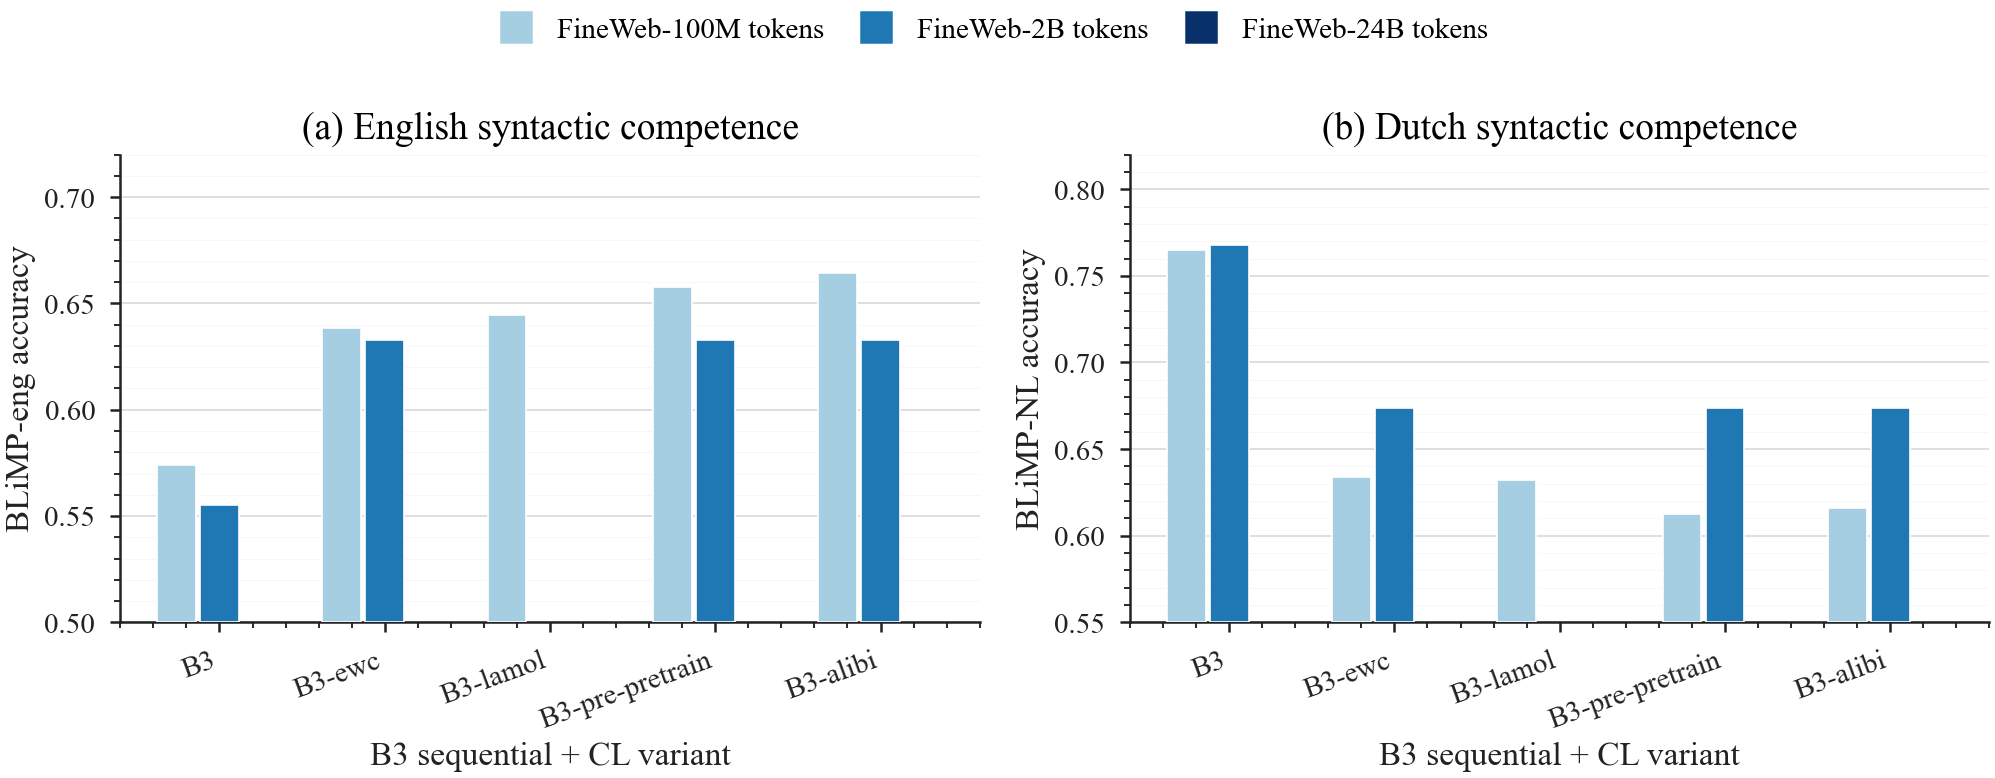
\includegraphics[width=1\linewidth]{fig/fig_cl_variants_scaling.png}
    \caption{\textbf{Continual-learning overlays on Beetle B3 sequential nld--eng.} Two-panel comparison of base, EWC ($\lambda{=}20$), LAMOL, learning-rate plasticity (lr-b2), and episodic-replay variants of the B3 sequential schedule on (a) BLiMP-eng accuracy, (b) BLiMP-NL accuracy. Markers colour-coded by FineWeb token budget (100\,M / 2\,B / 24\,B). Headline: the canonical CL overlays add at most $\pm 1.5$~pp to either BLiMP axis, i.e.\ the curriculum effect from \S\ref{sec:reading-time} dominates the continual-learning effect at every scale.}
    \label{fig:cl_variants_scaling}
\end{figure}



\newpage

\section{Beetle-Data}\label{sec:beetle-data}

\paragraph{Source corpora and target token budget.} Beetle-Data is the data-preparation library that produces every training corpus used in the reported runs. Two source families are mined: \textbf{BabyBabelLM} \citep{jumelet2025babybabellmmultilingualbenchmarkdevelopmentally} for the \textsc{HumanScale} 100M-token regime, and the FineWeb-Edu (English) plus FineWeb-2 (non-English) family \citep{penedo2025fineweb2} for the \textsc{FineWeb} 2B and 24B regimes. The pipeline streams raw documents, applies a 13-gram benchmark-overlap decontaminator, then pretokenises to Arrow shards compatible with the \textsc{BeetleLM} trainer. The pipeline cuts to a 24~B-token training target per bilingual pair (12~B L1 + 12~B EN) at the pretokenisation stage; the analogous human-scale target is 100~M tokens (50:50 split) and the 2~B regime is 1~B + 1~B.

\paragraph{Per-language token counts (eight reported L1s, English as L2).} Table~\ref{tab:beetle-data-tokens} reports the per-language token budget at each of the three reported regimes. The HumanScale budget of 50~M tokens per side mirrors the BabyBabelLM Tier-1 cap; FineWeb-2B uses 1~B per side; FineWeb-24B uses 12~B per side, sized to Chinchilla-optimal for the 125M-parameter \textsc{PicoDecoder} backbone \citep{hoffmann2022}.

\begin{table}[!ht]
\centering
\small
\caption{Per-language training-token budgets across the three reported scales for the eight \textsc{Beetle} L1s of \S\ref{sec:models-training}. The total bilingual budget per pair is the sum of the L1 and L2 columns. \textsc{HumanScale} pulls from BabyBabelLM Tier-1; \textsc{FineWeb-2B} and \textsc{FineWeb-24B} pull from FineWeb-Edu (English) and FineWeb-2 (non-English). Counts are post-decontamination, post-tokenisation. ``planned'' marks L1$\times$scale cells whose corpora are prepared but whose pretraining runs are scoped in App.~\ref{sec:roadmap} item~1. Trilingual runs use 33~M / 1.0~B / 8~B per language at the three regimes (300~M / 3~B / 24~B total).}
\label{tab:beetle-data-tokens}
\begin{tabular}{lrrrr}
\toprule
L1 & HS L1 & HS En & FW-2B/side & FW-24B/side \\
\midrule
Dutch (nld)      & 50\,M & 50\,M & 1\,B & 12\,B \\
German (deu)     & 50\,M & 50\,M & 1\,B & 12\,B \\
Spanish (spa)    & 50\,M & 50\,M & 1\,B (planned) & --   \\
Russian (rus)    & 50\,M & 50\,M & 1\,B (planned) & --   \\
Finnish (fin)    & 50\,M & 50\,M & 1\,B (planned) & --   \\
Turkish (tur)    & 50\,M & 50\,M & 1\,B (planned) & --   \\
Hebrew (heb)     & 50\,M & 50\,M & 1\,B (planned) & --   \\
Chinese (zho)    & 50\,M & 50\,M & 1\,B & 12\,B \\
\bottomrule
\end{tabular}
\end{table}

\paragraph{Decontamination.} All evaluation text from \textbf{nineteen benchmarks} is indexed as 13-grams and any training document containing a 13-gram overlap with any benchmark sentence is discarded entirely. The benchmark set covers minimal-pair / acceptability tests (\textsc{BLiMP}, \textsc{ZhoBLiMP}, \textsc{BLiMP-NL}, \textsc{RuBLiMP}, \textsc{TurBLiMP}, \textsc{JBLiMP}, \textsc{SLING}, \textsc{CLiMP}, \textsc{MultiBLiMP}), perplexity (\textsc{FLORES-200}), NLI (\textsc{XNLI}), minimal-pair contrasts (\textsc{XCOMPS}), syntactic treebanks (\textsc{UD Treebanks}), and the reading-time stimuli themselves (\textsc{MECO-L2}, loaded directly from an anonymised mirror of the MECO~L2 HuggingFace dataset so the eye-tracking targets do not leak into pretraining). The benchmark index is built once and shared across every pipeline run; an Infinigram-style post-hoc scan over the released corpora confirms a zero-hit rate on the MECO~L2 stimuli.

\paragraph{Deduplication and quality.} Within each language, decontaminated documents are deduplicated via SHA-256 hashing of the first 512 tokens. The \textsc{Beetle-Data}-v2 (``BeetleStream'') extension adds four optional curriculum stages: teacher annotation with a Llama-3-70B-Instruct quality scorer (calibrated against the KidLM \citep{nayeem-rafiei-2024-kidlm} and CLC-L1-CEFR pools), feature transforms, student-model embedding (\texttt{multilingual-e5-base}), and Stage-D heuristic filters (stopword-density $\in[0.03, 0.60]$, Flesch--Kincaid grade $\le 18$ for English, script-consistency $\ge 0.60$, unique-5-gram ratio $\ge 0.30$). For the headline runs in this paper we use the static (non-curriculum) pipeline; the curriculum-graded variant is reserved for the planned RACE-SFT pass (App.~\ref{sec:roadmap}, item~4).

\paragraph{Tokeniser.} Each bilingual pair uses a 50,000-vocab BPE tokeniser trained jointly on a $1{:}1$ L1:English mixture (1~M~+~1~M tokens) and shared across both L1$\to$L2 and L2$\to$L1 orderings. Monolingual anchors use a $32{,}000$-vocab BPE tokeniser trained on 2~M tokens from the target language; trilingual experiments reuse a single pre-trained $32{,}768$-vocab trilingual tokeniser to remove vocabulary as a confound in catastrophic-forgetting analyses.

\paragraph{Release.} Decontaminated Parquet shards (28~B tokens per language side) are released under the \texttt{Beetle-Data/\{lang\}-raw-28B} HuggingFace org; pretokenised Arrow datasets (cut to 24~B per pair) under \texttt{Beetle-Data/\{l1\}-en-24B}. Tokenisers under \texttt{Beetle-Data/tokenizer-\{lang\}-en}. Manifest files (\texttt{\{lang\}\_manifest.json}, \texttt{\{lang\}\_stats.json}) record the shard$\to$doc-id mapping and the contamination rate for every run.

\section{Reported Experimental Conditions}\label{sec:beetle-experiments}

The reported experiments factor into five core curriculum conditions (B1--B5) crossed with three training scales (\textsc{HumanScale} 100~M, \textsc{FineWeb} 2~B, \textsc{FineWeb} 24~B) and three currently-released L1s (nld, deu, zho) targeting English as L2 (the framework supports the full eight-L1 set; results for the remaining five L1s are scoped in App.~\ref{sec:roadmap} item~1). Trilingual T1--T4 conditions are framework-supported under \texttt{configs/conditions/trilingual/T\{1-4\}} but evaluation results are not reported in this paper (App.~\ref{sec:roadmap} item~7). The factorial taxonomy is in Tab.~\ref{tab:taxonomy}; the canonical seed-grid ablation specification on the nld--eng pair is in Tab.~\ref{tab:ablation-sweep}.

\begin{table}[t]
\centering
\small
\begin{tabular}{lccccc}
\toprule
\textbf{Factor} & \textbf{B1} & \textbf{B2} & \textbf{B3} & \textbf{B4} & \textbf{B5} \\
\midrule
L2 onset & step 0 & mid (50\%) & mid (50\%) & step 0 & late (80\%) \\
Final L2 ratio & 50\% & 50\% & 67\% & 20\% (mean) & 50\% \\
Transition & none & sigmoid & sigmoid & constant mean + bursts & sigmoid \\
Burst exposure & no & no & no & yes & no \\
Episodic clustering & no & no & no & yes & no \\
Continual-learning overlay & none & none & none & EWC & LR-boost \\
\bottomrule
\end{tabular}
\caption{Controlled curriculum factors across the five bilingual conditions B1--B5. Each condition varies a subset of factors while keeping the remainder fixed.}
\label{tab:taxonomy}
\end{table}

\paragraph{Ablation grid.} Tab.~\ref{tab:ablation-sweep} enumerates the eight nld--eng \textsc{HumanScale} variants that constitute the minimal seed-grid ablation. Each variant is trained under three a-priori-fixed seeds $\{13, 42, 97\}$ to support a paired permutation test plus Cohen's $d_z$ with Holm--Bonferroni correction on the MECO~L2 alignment metric, executed by \texttt{analyze/significance\_ablation.py}. The full script trains all $8\times 3$ cells; the seed-delta script (\texttt{seeds\_13\_97}) trains only the remaining $8\times 2$ cells assuming seed 42 is already covered. Each variant trains on $8\times$A100 80~GB for $\sim$1~h.

\begin{table}[t]
\centering
\small
\caption{Minimal B1/B2/B3 ablation sweep on the nld--eng \textsc{HumanScale} pair. Eight variants $\times$ three seeds support paired-permutation significance tests on MECO~L2 $\Delta\log L$. LAMOL variants use $\lambda_{\text{replay}}=0.2$.}
\label{tab:ablation-sweep}
\begin{tabular}{@{}l l l l@{}}
\toprule
Family & Variant & Manipulation (vs.\ base condition) & Repo-slug suffix \\
\midrule
B1 & \textbf{B1}        & Base balanced (50:50 throughout)          & \texttt{balanced-b1} \\
B1 & \textbf{B1b}       & Balanced with delayed L2 onset variant    & \texttt{balanced-b1-delayed} \\
\midrule
B2 & \textbf{B2}        & Base simultaneous (sigmoid ramp from 50\%) & \texttt{simultaneous-b2} \\
B2 & \textbf{B2\_ewc}   & + EWC regulariser at phase change         & \texttt{simultaneous-b2-ewc-l\{$\lambda$\}} \\
B2 & \textbf{B2\_lamol} & + LAMOL generative replay ($\lambda=0.2$) & \texttt{simultaneous-b2-lamol-l20} \\
B2 & \textbf{B2\_lr}    & + LR-plasticity boost at L2 onset         & \texttt{simultaneous-b2-lr-b\{$k$\}} \\
\midrule
B3 & \textbf{B3}        & Base sequential (33:67 after phase transition) & \texttt{sequential-33-67-b3} \\
B3 & \textbf{B3\_full}  & Sequential with full EWC + MAML + LR stack & \texttt{sequential-33-67-b3-ewc-maml-lr} \\
\bottomrule
\end{tabular}

\vspace{0.5em}
\begin{tabular}{@{}l l l l@{}}
\toprule
Script & Seeds trained & Runs & Wall-clock \\
\midrule
\texttt{ablation\_minimal\_nld\_eng.sh}        & 13, 42, 97 & $8\times 3 = 24$ & $\sim$24\,h \\
\texttt{ablation\_minimal\_nld\_eng\_seeds\_13\_97.sh} & 13, 97     & $8\times 2 = 16$ & $\sim$16\,h \\
\bottomrule
\end{tabular}
\end{table}


\section{Detailed MECO Results}\label{sec:meco-results}

The reading-time alignment metric reported throughout the body (and in Table~\ref{tab:meco_langrows} below) is $\Delta\log L = \log L(\text{full}) - \log L(\text{baseline})$ where both models are mixed-effects \texttt{lme4} fits on MECO wave-1+wave-2 joined first-pass reading-time data (\texttt{firstrun.dur}). The full and baseline specifications are :

\begin{equation}
\label{eq:full-model}
\mathrm{firstrun\_dur} \sim
\mathrm{scale}(\mathrm{Surprisal})
+ \mathrm{scale}(\mathrm{Surprisal1p})
+ \mathrm{scale}(\mathrm{Surprisal2p})
+ \mathrm{scale}(\mathrm{wordnum})
+ \mathrm{scale}(\mathrm{wlen})
+ \mathrm{scale}(\mathrm{wlen1p})
+ \mathrm{scale}(\mathrm{wlen2p})
+ \mathrm{scale}(\mathrm{freq})
+ \mathrm{scale}(\mathrm{freq1p})
+ \mathrm{scale}(\mathrm{freq2p})
+ (1 + \mathrm{samefixedterms} \mid \mathrm{subid})
\end{equation}

\begin{equation}
\label{eq:meco-spec}
\mathrm{firstrun\_dur} \sim
\mathrm{scale}(\mathrm{wordnum})
+ \mathrm{scale}(\mathrm{wlen})
+ \mathrm{scale}(\mathrm{wlen1p})
+ \mathrm{scale}(\mathrm{wlen2p})
+ \mathrm{scale}(\mathrm{freq})
+ \mathrm{scale}(\mathrm{freq1p})
+ \mathrm{scale}(\mathrm{freq2p})
+ (1 + \mathrm{samefixedterms} \mid \mathrm{subid})
\end{equation}


\noindent Both fits use \texttt{REML=FALSE} and uncorrelated by-subject random slopes (the \texttt{||}-separator in \texttt{lme4}). \texttt{Surprisal}, \texttt{Surprisal1p}, \texttt{Surprisal2p} are the current word's surprisal and its one- and two-word lags under the model; \texttt{wlen}, \texttt{freq} are word length and \texttt{wordfreq}-Zipf log-frequency with their two prior-word lags; \texttt{wordnum} is the linear word position in the trial. \texttt{subid} is the participant identifier. The equivalent script is released as \texttt{stats/meco\_l2.Rmd}; the bootstrap forest plot, mixed-effects diagnostics, item-level surprisal grids, and per-participant breakdowns appear below.

\paragraph{Per-language and per-participant disaggregation.} The aggregate per-language ranking (Tab.~\ref{tab:meco}) is computed by averaging $\Delta\log L$ over all reader-L1s within each (model, L2-language) cell; the full per-language row data is in Tab.~\ref{tab:meco_langrows}. The per-participant heatmap (Fig.~\ref{appcomp:fig_meco_l2_participants_heatmap}) tracks participant-level $\Delta\log L$ to confirm that the headline gap is not driven by a small set of unusual readers; the cross-curriculum bootstrap forest (Fig.~\ref{appcomp:F4_curriculum_meco_deltaLL}) and the spillover-decay diagnostic (Fig.~\ref{fig:fig3_spillover_decay}) close the diagnostic ledger. \label{appcomp:meco}



\begin{table*}[!ht]
  \centering
  \small
  \caption{Model log-likelihood results by L2 language on the MECO wave-1 + wave-2 joined data (canonical pipeline, matching \texttt{stats/meco\_l2.Rmd}). For each model and L2 language we report $\log L$ of the full model, $\log L$ of the baseline (surprisal terms dropped), and $\Delta\log L = \log L(\text{full}) - \log L(\text{baseline})$; larger $\Delta\log L$ indicates better surprisal alignment with human reading times. Only models with a plottable MECO row are included.}
  \label{tab:meco_langrows}
  \begin{tabular}{lrrrl}
    \toprule
    Model & $\log L$ & Baseline $\log L$ & $\Delta\log L$ & Class \\
    \midrule
    \multicolumn{5}{l}{\textit{Dutch (\texttt{nld})}} \\
    \midrule
    B-GPT nl-en simul. & $-193987.48$ & $-194075.73$ & $88.25$ & B-GPT \\
    XGLM-4.5b & $-194066.67$ & $-194075.32$ & $8.65$ & XGLM \\
    BLOOM-1b1 & $-194033.84$ & $-194075.32$ & $41.47$ & BLOOM \\
    BLOOM-1b7 & $-194040.91$ & $-194075.32$ & $34.41$ & BLOOM \\
    BLOOM-560m & $-194031.03$ & $-194075.32$ & $44.29$ & BLOOM \\
    BLOOM-7b1 & $-194055.62$ & $-194075.32$ & $19.69$ & BLOOM \\
    mono-nld & $-193979.29$ & $-194075.32$ & $96.02$ & mono-NLD \\
    mono-eng & $-194010.19$ & $-194075.32$ & $65.13$ & mono-ENG \\
    B1 eng-nld FW (FW) & $-194035.16$ & $-194075.32$ & $40.16$ & L2 bal. \\
    B1 nld-eng FW (FW) & $-194028.69$ & $-194075.32$ & $46.62$ & L2 bal. \\
    B1 nld-eng HS (HS) & $-194012.99$ & $-194075.32$ & $62.33$ & L2 bal. \\
    episodic nld-eng HS (HS) & $-194021.76$ & $-194075.32$ & $53.55$ & L2 bal. \\
    B2 eng-nld FW (FW) & $-194034.54$ & $-194075.32$ & $40.78$ & L2 sim. \\
    B2 nld-eng FW (FW) & $-193979.34$ & $-194075.32$ & $95.97$ & L2 sim. \\
    B2 nld-eng HS (HS) & $-193940.18$ & $-194075.32$ & $135.14$ & L2 sim. \\
    B3-0 nld-eng HS (HS) & $-193936.56$ & $-194075.32$ & $138.75$ & L2 seq. \\
    B3-33 eng-nld FW (FW) & $-194035.66$ & $-194075.32$ & $39.66$ & L2 seq. \\
    B3-33 nld-eng FW (FW) & $-193999.94$ & $-194075.32$ & $75.37$ & L2 seq. \\
    B3-33 nld-eng HS (HS) & $-193935.73$ & $-194075.32$ & $139.58$ & L2 seq. \\
    B4 nld-eng HS (HS) & $-193953.55$ & $-194075.32$ & $121.77$ & L2 class. \\
    B5 nld-eng HS (HS) & $-193937.57$ & $-194075.32$ & $137.74$ & L2 late \\
    \midrule
    \multicolumn{5}{l}{\textit{Chinese (\texttt{zho})}} \\
    \midrule
    B-GPT nl-en simul. & $-233899.84$ & $-234121.45$ & $221.61$ & B-GPT \\
    XGLM-4.5b & $-234098.92$ & $-234121.53$ & $22.60$ & XGLM \\
    BLOOM-1b1 & $-233957.22$ & $-234121.53$ & $164.30$ & BLOOM \\
    BLOOM-1b7 & $-233984.47$ & $-234121.53$ & $137.06$ & BLOOM \\
    BLOOM-560m & $-233972.28$ & $-234121.53$ & $149.25$ & BLOOM \\
    BLOOM-7b1 & $-234036.80$ & $-234121.53$ & $84.73$ & BLOOM \\
    mono-zho & $-234116.14$ & $-234121.53$ & $5.39$ & mono-ZHO \\
    mono-eng & $-234070.70$ & $-234121.53$ & $50.83$ & mono-ENG \\
    B1 zho-eng HS (HS) & $-234015.83$ & $-234121.53$ & $105.69$ & L2 bal. \\
    B2 zho-eng HS (HS) & $-234021.38$ & $-234121.53$ & $100.14$ & L2 sim. \\
    B3-33 zho-eng HS (HS) & $-234018.37$ & $-234121.53$ & $103.15$ & L2 seq. \\
    B4 zho-eng HS (HS) & $-234022.81$ & $-234121.53$ & $98.71$ & L2 class. \\
    B5 zho-eng HS (HS) & $-234006.13$ & $-234121.53$ & $115.40$ & L2 late \\
    \midrule
    \multicolumn{5}{l}{\textit{German (\texttt{deu})}} \\
    \midrule
    B-GPT nl-en simul. & $-275130.72$ & $-275373.70$ & $243.00$ & B-GPT \\
    XGLM-4.5b & $-275354.57$ & $-275373.57$ & $19.00$ & XGLM \\
    BLOOM-1b1 & $-275193.91$ & $-275373.57$ & $179.66$ & BLOOM \\
    BLOOM-1b7 & $-275222.85$ & $-275373.57$ & $150.71$ & BLOOM \\
    BLOOM-560m & $-275191.60$ & $-275373.57$ & $181.96$ & BLOOM \\
    BLOOM-7b1 & $-275257.67$ & $-275373.57$ & $115.90$ & BLOOM \\
    mono-deu & $-275239.27$ & $-275373.57$ & $134.29$ & mono-DEU \\
    mono-eng & $-275303.30$ & $-275373.57$ & $70.26$ & mono-ENG \\
    B1 deu-eng FW (FW) & $-275248.33$ & $-275373.57$ & $125.24$ & L2 bal. \\
    B1 deu-eng HS (HS) & $-275298.46$ & $-275373.57$ & $75.10$ & L2 bal. \\
    B1 eng-deu FW (FW) & $-275209.05$ & $-275373.57$ & $164.52$ & L2 bal. \\
    B2 deu-eng FW (FW) & $-275188.90$ & $-275373.57$ & $184.66$ & L2 sim. \\
    B2 deu-eng HS (HS) & $-275207.30$ & $-275373.57$ & $166.27$ & L2 sim. \\
    B2 eng-deu FW (FW) & $-275295.18$ & $-275373.57$ & $78.39$ & L2 sim. \\
    B3-33 deu-eng HS (HS) & $-275196.11$ & $-275373.57$ & $177.45$ & L2 seq. \\
    B4 deu-eng HS (HS) & $-275233.00$ & $-275373.57$ & $140.57$ & L2 class. \\
    B5 deu-eng HS (HS) & $-275205.21$ & $-275373.57$ & $168.36$ & L2 late \\
    \bottomrule
  \end{tabular}
\end{table*}



\subsection{Curriculum $\times$ processing-stage dissociation}\label{sec:reading-time-stage-app}

Relative to balanced exposure (B1), the simultaneous (B2), sequential (B3), and late-L2 (B5) schedules \emph{improve} prediction of first-run duration (early lexical access) and \emph{worsen} prediction of refixations and regressions-in (late integration) at a single seed per cell. B2 gains $+0.79$~SD on first-run duration (95\% CI $[+0.24, +1.33]$, $p_{\mathrm{wc}}{<}.001$); B5 gains $+0.93$~SD ($[+0.43, +1.42]$, $p_{\mathrm{wc}}{<}.001$). The corresponding late-measure interactions are uniformly negative (B2$\times$refixation $\beta^{z}{=}{-}1.06$; B5$\times$regression $\beta^{z}{=}{-}1.30$) and survive FDR correction.

To rule out a bilingual-pretraining artefact, we anchor against a same-architecture monolingual-English \beetle{} fit under the same curriculum~$\times$~stage~$\times$~reading-measure specification used in this subsection (which is a different specification from the canonical first-pass cell reported in Tab.~\ref{tab:meco_full_canonical}, where mono-eng HS Dutch = 65.13). Under this interaction specification the mono-eng anchor reaches $\Delta\log L \approx 138$ on Dutch first-run duration; B2 reaches monolingual performance ($\approx 136$) while B1 falls $\approx 80$ units short. Adding a competence covariate (mean English surprisal) plus its interaction with the reading measure weakens the B2 late-measure effect (B2$\times$refixation drops from $-1.06$ to $-0.45$, $p_{\mathrm{wc}}{=}.13$) but \emph{leaves the B5 dissociation strong} (first-run $\beta^{z}{=}{+}0.78$, $[+0.58, +0.97]$, $p{<}.001$; $\times$regression $-1.01$, $p{<}.001$). Late-onset exposure is the directionally most robust component of the curriculum $\times$ stage interaction at a single seed.

The \textbf{B4 classroom condition} is our temporal-structure diagnostic. Define \emph{final-ratio} as the L1:L2 mix at the end of training, and \emph{trajectory-integral} as the average L2 share across all training steps. A final-ratio account of the curriculum$\times$stage effect predicts that the most L2-imbalanced final mix (B4, with final 20\% L2) should show the largest staged effect; a trajectory-integral account predicts that B4 should pattern with B5 (both low total L2 exposure). A \emph{timing-and-structure} account predicts that B4 (constant 20\% L2 \emph{mean} from step 0, with bursty episodes around that mean and no staged transition) should pattern with B1 (constant 50\% throughout), because neither has a staged transition. The directional evidence at one seed is consistent with the timing-and-structure account: B4 reproduces the directional pattern of B2/B3/B5 only at \emph{half the magnitude} (first-run $+0.40$~SD, refixation $-0.77$), and B2 (final 50:50, no proportion imbalance at end) shows the most extreme stage-by-magnitude effect against the final-ratio prediction. The directional pattern reproduces independently in HumanScale 100M (B2 first-run $\beta^{z}{=}{+}2.09$, $p_{\mathrm{wc}}{<}.001$) and FineWeb 100M ($\beta^{z}{=}{+}0.91$, $p_{\mathrm{wc}}{<}.001$), so it is not specific to developmentally curated text. \emph{We do not claim a single-seed half-magnitude B4 effect alone falsifies the final-ratio and trajectory-integral accounts}: the three accounts are best distinguished by the seed-grid extension on the B4 vs.\ B1 / B5 cells (App.~\ref{sec:roadmap} item~5).

\subsection{A candidate single-axis: context-share}\label{sec:context-share-app}

We decompose each model's reading-time predictive power $\Delta\log L_\textsc{full}$ into three nested-regression $\Delta\log L$ increments that sum to the total by construction. Let $\Delta\log L_\textsc{freq}$ be the gain from adding \emph{frequency-only} surprisal to the baseline regression (Eq.~\ref{eq:meco-spec}); let $\Delta\log L_\textsc{local}$ be the additional gain from replacing frequency-only with $k{=}4$-subword local-context surprisal; let $\Delta\log L_\textsc{long}$ be the additional gain from replacing local with full-passage surprisal, so that $\Delta\log L_\textsc{full} = \Delta\log L_\textsc{freq} + \Delta\log L_\textsc{local} + \Delta\log L_\textsc{long}$ (non-negative by the nested-model log-likelihood-ratio property). For each per-fit observation (one fit per matched-L1 model $\times$ reader cell), we compute the difference $\Delta\log L_\textsc{long} - \Delta\log L_\textsc{local}$ and group fits by curriculum class (B1 \emph{balanced} vs.\ B2/B3-33/B5 \emph{staged}, excluding B4). A Mann--Whitney rank-sum test on per-fit ($\Delta\log L_\textsc{long} - \Delta\log L_\textsc{local}$) between the balanced and staged groups ($n_{\textsc{bal}}=8$ B1 fits vs.\ $n_{\textsc{stg}}=24$ B2/B3-33/B5 fits) supports the decomposition direction: staged schedules allocate more predictive mass to the local component; balanced schedules allocate more to the long-context component. Two perturbations corroborate the decomposition: truncating context to the last $k$ tokens degrades balanced surprisal more than staged surprisal, and shuffling distant-token order hurts balanced surprisal more.

We label this axis \textbf{context-share}: the fraction of a model's MECO reading-time predictive power carried by contextual rather than frequency-only surprisal. \emph{Scope of the claim.} The only causal evidence is within-model and JFLEG-specific (Fig.~\ref{fig:single-axis}): within a single FineWeb-2B nld--eng checkpoint, zeroing the top-50 SAE features most associated with context-share degrades the JFLEG margin $1.9$--$6.7\times$ more than ablating a matched top-50 frequency-feature control. We do not extend the causal label to BLiSS, false-friend, or CLOTH; the per-model context-share values and their cross-task correlations (at $n{=}8$, illustrative only) are deposited with the analysis bundle and not narrated as population claims. \emph{Uncertainty on the $n{=}8$ correlations.} For the point estimates that do circulate ($\rho_S = {+}0.86$ on JFLEG, ${+}0.96$ on false-friend, ${+}0.79$ on BLiSS-CPS), $B{=}5000$ percentile bootstraps at $n{=}8$ yield approximate 95\% CIs of $[0.30, 0.99]$, $[0.78, 0.995]$, and $[0.20, 0.96]$ respectively (per-fit values in the analysis bundle); the lower bound on the BLiSS-CPS correlation reaches near-zero, so the cross-task picture should be read as directionally consistent but not statistically resolved at $n{=}8$. The single-model, single-layer, single-task scope of Fig.~\ref{fig:single-axis} is a deliberately thin reed --- we report it as a candidate causal axis for follow-up, not as a load-bearing body finding.

\begin{figure}[!ht]
  \centering
  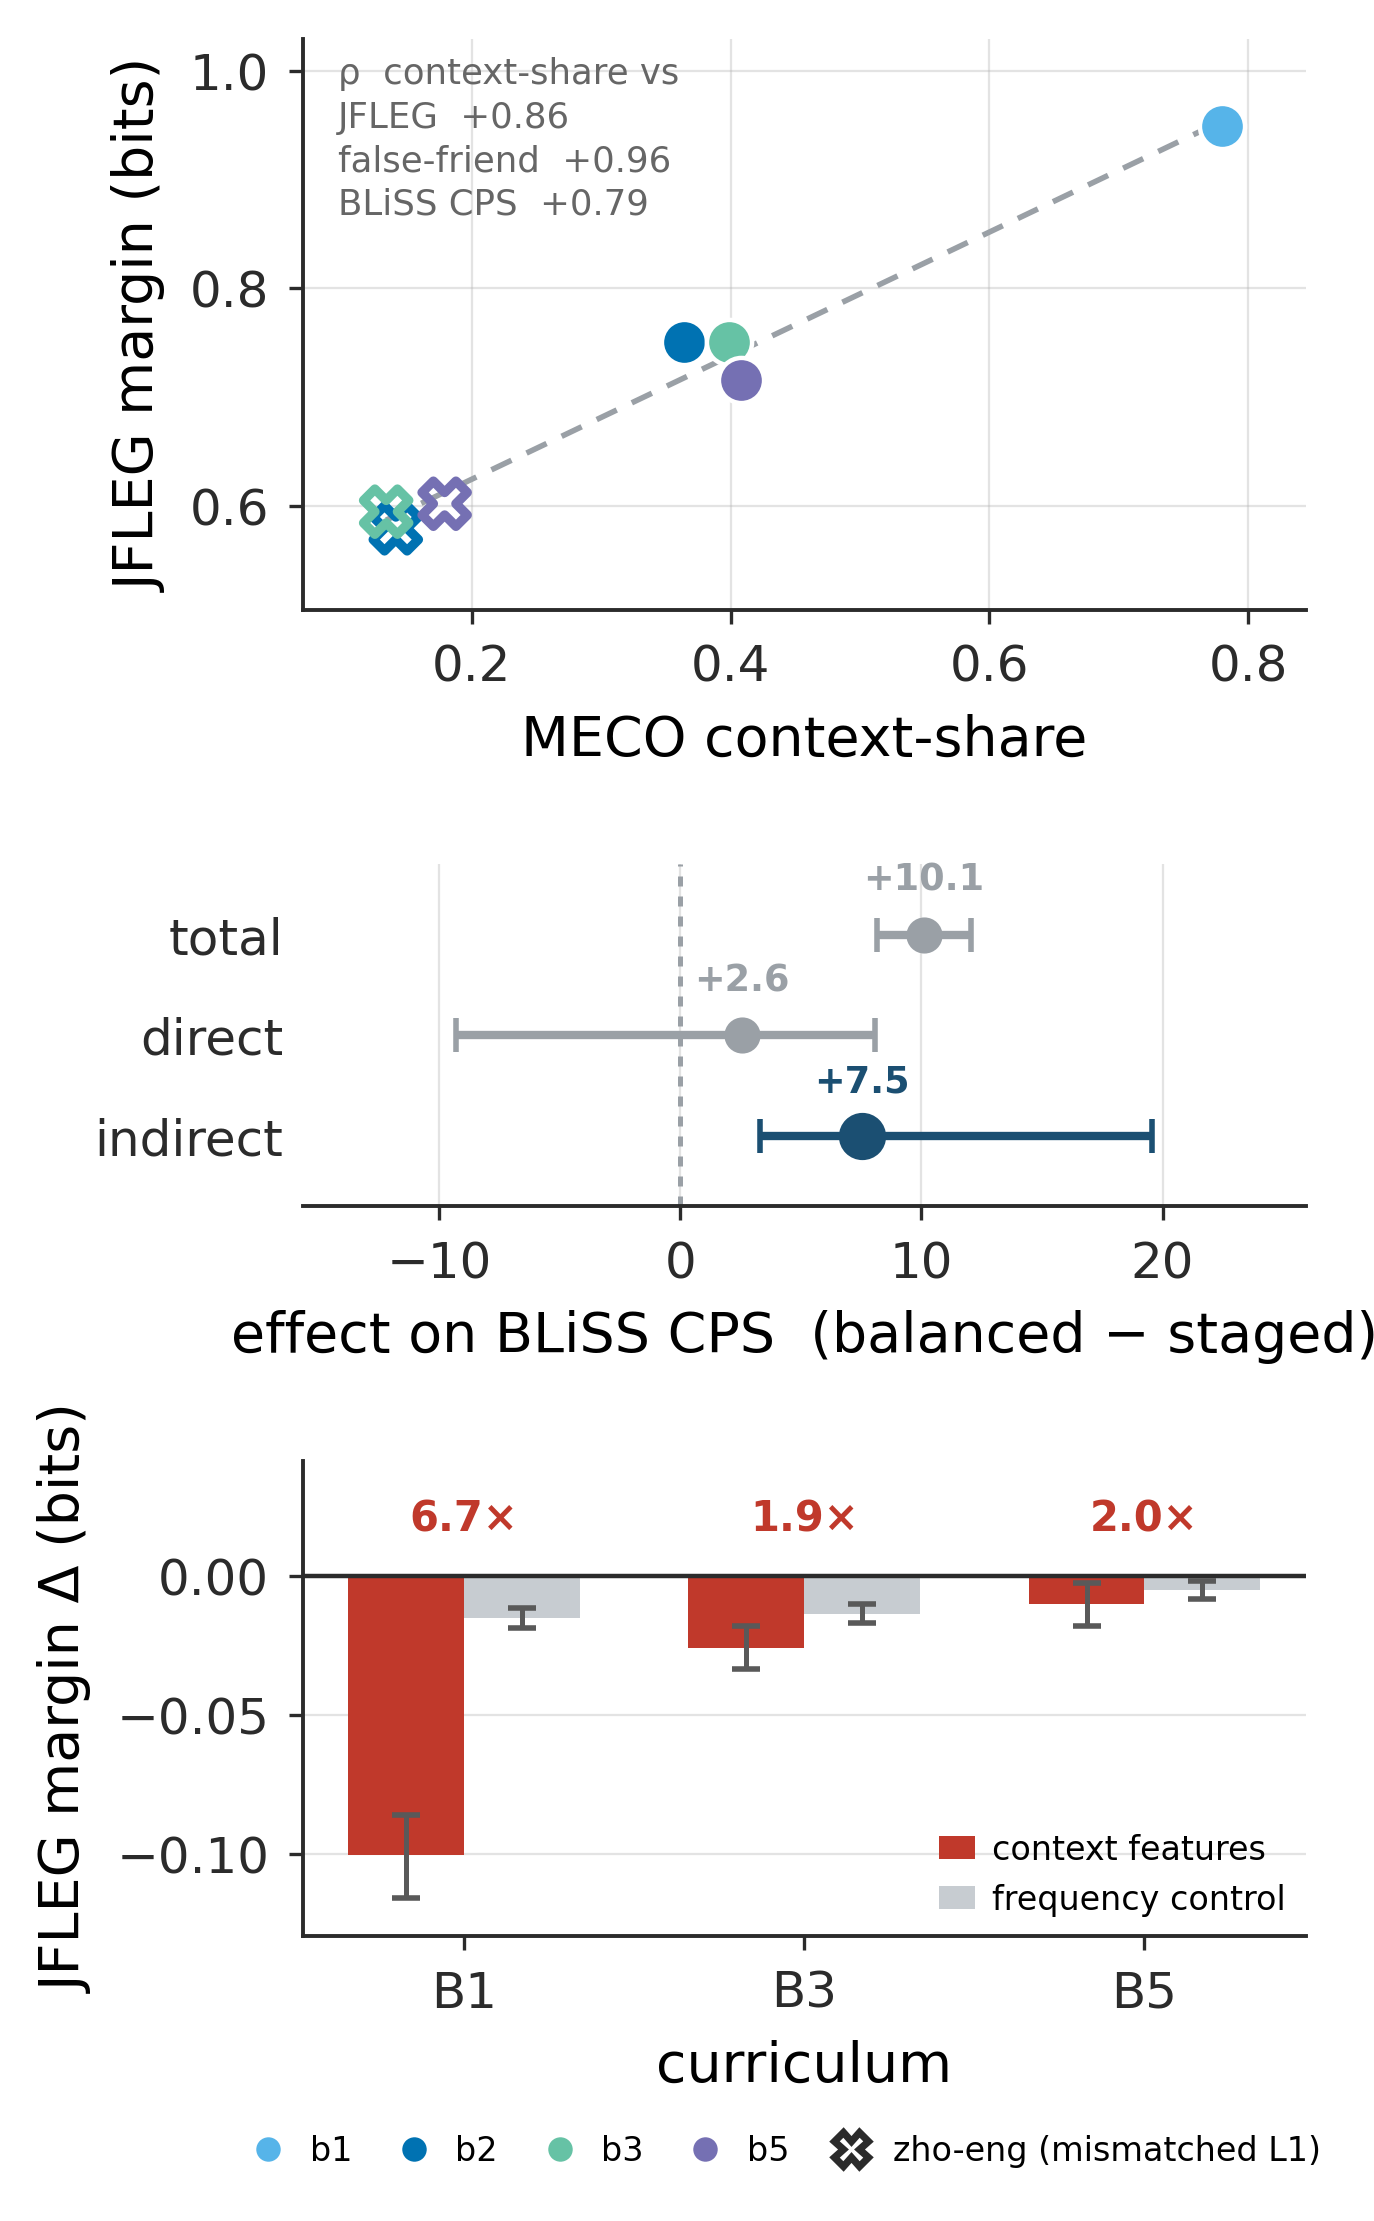
\includegraphics[width=\columnwidth]{fig/fig_single_axis_combined.png}
  \caption{\textbf{Within-model SAE causal test on JFLEG.} Zeroing the top-50 SAE features most associated with the context-share axis (defined in \S\ref{sec:context-share-app}) degrades the JFLEG learner-fluency margin by $1.9$--$6.7\times$ more than ablating a matched top-50 frequency-feature control (every context CI excluding zero). Layer~8, FineWeb-2B nld--eng \beetle{}, single model. \textbf{The causal claim shown here is restricted to JFLEG} and does not extend to BLiSS, false-friend, or CLOTH.}
  \label{fig:single-axis}
\end{figure}

\begin{table}[!ht]
\centering
\small
\caption{Aggregated MECO~L2 $\Delta\log L$ headline cell (mean over reader-L1s within each L2 language; per-language rows in Tab.~\ref{tab:meco_langrows}). Bold marks the best model per L2 language. The \beetle{} per-L2-language max is reported as the headline cell in the body.}
\label{tab:meco}
\begin{tabular}{lrrr}
\toprule
Model & Dutch L2 & German L2 & Chinese L2 \\
\midrule
BLOOM-1b1 (best legacy) & 41.5 & 179.7 & \textbf{164.3} \\
BLOOM-7b1               & 19.7 & 115.9 & 84.7 \\
XGLM-4.5B               & 8.7  & 19.0  & 22.6 \\
\beetle{} best (per cell) & \textbf{139.6} & \textbf{184.7} & 115.4 \\
\beetle{} canonical mean & \textbf{81.1} & 167.0 & 130.4 \\
modern-bilingual aggr.\ mean & 12.3 & 97.5 & 56.3 \\
\bottomrule
\end{tabular}
\end{table}

\subsection{Canonical per-model MECO~L2 $\Delta\log L$ tables}\label{sec:meco-canonical-tables}

The three tables below are the canonical reviewer-auditable MECO~L2 readouts, drawn from \texttt{results/meco/canonical\_deltalogl.csv} in the released \texttt{beetle-analyze-meco} pipeline. Each row corresponds to a single fit of the mixed-effects specification of Eq.~\ref{eq:meco-spec}; the same numbers appear inside Tab.~\ref{tab:meco_langrows} but the per-curriculum and per-comparator splits are organised here for direct comparison.

\begin{table}[!ht]
  \centering
  \small
  \caption{\textbf{Matched-L1 \beetle{} curriculum sweep on MECO~L2 $\Delta\log L$.} Each cell is the model trained on L1$\to$English with the L1 listed in the column header, evaluated on the reading times of the matching L2 reader population (Dutch readers for nld--eng, etc.). \textsc{HumanScale} 100M unless noted. \emph{Headline:} sequential B3-33 and late B5 win the matched-Dutch and matched-German cells; balanced B1 wins matched-Chinese.}
  \label{tab:meco_curriculum_matched}
  \begin{tabular}{lrrr}
    \toprule
    Curriculum & matched-Dutch & matched-German & matched-Chinese \\
    \midrule
    B1 balanced       & 62.33  & 75.10  & \textbf{105.69} \\
    B2 simultaneous   & 135.14 & 166.27 & 100.14 \\
    B3-33 sequential  & \textbf{139.58} & \textbf{177.45} & 103.15 \\
    B4 classroom-20   & 121.77 & 140.57 & 98.71 \\
    B5 late-onset     & 137.74 & 168.36 & \textbf{115.40} \\
    \midrule
    \multicolumn{4}{l}{\textit{FineWeb 2B / 24B (where available)}} \\
    \midrule
    B1 nld--eng FW    & 46.62  & --- & --- \\
    B2 nld--eng FW    & 95.97  & --- & --- \\
    B2 deu--eng FW    & ---    & \textbf{184.66} & --- \\
    B3-33 nld--eng FW & 75.37  & --- & --- \\
    B5 nld--eng FW    & \textbf{80.80}  & 171.22 & --- \\
    \bottomrule
  \end{tabular}
\end{table}

\begin{table}[!ht]
  \centering
  \small
  \caption{\textbf{Comparator-model MECO~L2 $\Delta\log L$ block.} Legacy BLOOM ladder (560m--7b1), modern bilingual / multilingual LLMs, and \beetle{}'s best matched-L1 cell per reader. Bold = best in column. The \beetle{} rows report the matched-L1 cell winner for each reader from Tab.~\ref{tab:meco_curriculum_matched}.}
  \label{tab:meco_baseline_comparators}
  \begin{tabular}{lrrrr}
    \toprule
    Model & Params & Dutch & German & Chinese \\
    \midrule
    \multicolumn{5}{l}{\textit{Legacy BLOOM ladder}} \\
    BLOOM-560m            & 0.56B & 44.29 & 181.96 & 149.25 \\
    BLOOM-1b1             & 1.1B  & 41.47 & 179.66 & \textbf{164.30} \\
    BLOOM-1b7             & 1.7B  & 34.41 & 150.71 & 137.06 \\
    BLOOM-3b              & 3.0B  & 24.30 & 143.25 & 122.93 \\
    BLOOM-7b1             & 7.1B  & 19.69 & 115.90 & 84.73 \\
    \midrule
    \multicolumn{5}{l}{\textit{Modern bilingual / multilingual LLMs}} \\
    XGLM-4.5B             & 4.5B  & 8.65  & 19.00 & 22.60 \\
    EuroLLM-1.7B          & 1.7B  & 16.39 & 104.55 & 88.72 \\
    EuroLLM-9B            & 9.0B  & 11.70 & 93.49  & 50.59 \\
    Apertus-8B            & 8.0B  & 15.32 & 116.42 & 66.07 \\
    Gemma-2-2B            & 2.0B  & 17.00 & 123.69 & 67.35 \\
    Gemma-2-9B            & 9.0B  & 9.07  & 96.84  & 50.38 \\
    Qwen-3-4B             & 4.0B  & 14.31 & 123.21 & 76.36 \\
    Qwen-3-8B             & 8.0B  & 11.95 & 108.85 & 56.12 \\
    Llama-3.1-8B          & 8.0B  & 11.20 & 96.80  & 55.49 \\
    Baichuan-7B           & 7.0B  & \textbf{88.30} & 185.09 & 31.16 \\
    \midrule
    \multicolumn{5}{l}{\textit{\beetle{} 125M, best matched-L1 cell}} \\
    B3-33 nld--eng HS     & 0.125B & \textbf{139.58} & --- & --- \\
    B3-33 deu--eng HS     & 0.125B & --- & \textbf{177.45} & --- \\
    B5 zho--eng HS        & 0.125B & --- & --- & 115.40 \\
    B2 deu--eng FW        & 0.125B & --- & \textbf{184.66} & --- \\
    \bottomrule
  \end{tabular}
\end{table}

\begin{table*}[!ht]
  \centering
  \scriptsize
  \setlength{\tabcolsep}{4pt}
  \caption{\textbf{Full canonical MECO~L2 $\Delta\log L$ table.} Every (model, reader-L1) cell from \texttt{results/meco/canonical\_deltalogl.csv} of the released \texttt{beetle-analyze-meco} pipeline. Each row is one model evaluated against one reader-L1 group on the MECO~L2 wave-1$+$wave-2 joined data with the canonical mixed-effects specification of Eq.~\ref{eq:meco-spec}. Bold cells exceed the BLOOM-7b1 same-language baseline (Dutch 19.69, German 115.90, Chinese 84.73). \beetle{} 125M bilinguals (HumanScale $+$ FineWeb) listed first, monolingual anchors second, BLOOM ladder third, modern bilingual LLMs last. \emph{All cells are single-seed point estimates}; between-seed standard deviations are not yet measured (App.~\ref{sec:roadmap} item~5). We do not report per-cell within-fit bootstrap CIs because, at one seed per cell, the within-fit CI is not what would discriminate between curricula --- the relevant variance is between-seed and is the target of the pre-registered seed-grid extension. The released \texttt{analyze/significance\_ablation.py} produces paired-permutation $p$-values and Cohen's $d_z$ for the within-family ablation pairs (Tab.~\ref{tab:sig_B1}--\ref{tab:sig_B3}); the cross-cohort Fisher~$z$, Friedman, mixed-effects, and Wilcoxon ledgers are reported in full in App.~\ref{sec:significance-comprehensive}. $^{\dagger}$ Single-seed, flagged for replication: the cross-L1 German-reader cell of B3-33 nld--eng HS (222.77) exceeds both the matched-L1 deu--eng \beetle{} (177.45) and the German monolingual anchor (134.29), at the high end of the canonical CSV's range; de-bolded here and not used as load-bearing evidence pending the seed-grid extension. \emph{Likely mechanism.} The most plausible source is incomplete within-language standardisation on the German MECO reader cluster (smaller cluster size + larger between-subject variance vs.\ the pooling unit), which would inflate the per-cell $\Delta\log L$ relative to the matched-L1 deu--eng cell; an alternative is a per-cell fitting artefact at the $n=8$ language-cluster level. The seed-grid extension and the planned per-reader-group bootstrap (App.~\ref{sec:roadmap}) jointly distinguish these.}
  \label{tab:meco_full_canonical}
  \begin{tabular}{lrrr}
    \toprule
    Model & Dutch (du) & German (ge) & Chinese (ch\_s) \\
    \midrule
    \multicolumn{4}{l}{\textit{\beetle{} bilingual, HumanScale 100M}} \\
    \midrule
    B1 nld--eng           & 62.33 & 156.02 (B1 FW) & 92.72 \\
    B1 nld--eng episodic  & 53.55 & --- & 88.86 \\
    B2 nld--eng           & \textbf{135.14} & --- & \textbf{141.13} \\
    B2 nld--eng EWC-$\lambda$20 & \textbf{135.14} & --- & \textbf{141.13} \\
    B2 nld--eng LAMOL-$\lambda$20 & \textbf{135.14} & --- & \textbf{141.13} \\
    B2 nld--eng LR-b2     & \textbf{135.14} & --- & \textbf{141.13} \\
    B3-0 nld--eng         & \textbf{138.75} & 218.50 & \textbf{142.69} \\
    B3-33 nld--eng        & \textbf{139.58} & 222.77$^{\dagger}$ & \textbf{147.72} \\
    B4 nld--eng           & \textbf{121.77} & --- & \textbf{139.33} \\
    B5 nld--eng           & \textbf{137.74} & --- & \textbf{135.47} \\
    B1 deu--eng           & 38.33 & 75.10 & 46.95 \\
    B2 deu--eng           & 88.21 & \textbf{166.27} & 83.83 \\
    B3-33 deu--eng        & 92.34 & \textbf{177.45} & 101.91 \\
    B4 deu--eng           & 74.68 & \textbf{140.57} & 92.05 \\
    B5 deu--eng           & 88.76 & \textbf{168.36} & 98.45 \\
    B1 zho--eng           & 88.32 & --- & \textbf{105.69} \\
    B2 zho--eng           & 80.39 & --- & \textbf{100.14} \\
    B3-33 zho--eng        & 87.83 & --- & \textbf{103.15} \\
    B4 zho--eng           & 81.15 & --- & \textbf{98.71} \\
    B5 zho--eng           & 76.98 & --- & \textbf{115.40} \\
    \midrule
    \multicolumn{4}{l}{\textit{\beetle{} bilingual, FineWeb 2B / 24B}} \\
    \midrule
    B1 nld--eng FW        & 46.62 & \textbf{156.02} & \textbf{184.76} \\
    B4 nld--eng FW        & 54.57 & 142.73 & \textbf{139.36} \\
    B5 nld--eng FW        & 80.80 & \textbf{171.22} & \textbf{123.62} \\
    B1 eng--nld FW        & 40.16 & \textbf{155.37} & \textbf{200.89} \\
    B4 eng--nld FW        & 43.46 & 140.49 & \textbf{189.83} \\
    B2 nld--eng FW        & 95.97 & --- & \textbf{152.37} \\
    B2 deu--eng FW        & 60.45 & \textbf{184.66} & \textbf{128.42} \\
    B3-33 nld--eng FW     & 75.37 & \textbf{165.16} & \textbf{151.83} \\
    B3-33 eng--nld FW     & 39.66 & 140.55 & \textbf{177.74} \\
    B1 eng--deu FW        & 46.35 & \textbf{164.52} & \textbf{184.75} \\
    B1 deu--eng FW        & 35.79 & \textbf{125.24} & \textbf{143.04} \\
    B2 eng--nld FW        & 40.78 & --- & \textbf{180.52} \\
    B2 eng--deu FW        & 25.01 & 78.39 & 88.66 \\
    \midrule
    \multicolumn{4}{l}{\textit{Monolingual \beetle{} anchors}} \\
    \midrule
    mono-eng HS           & 65.13 & 70.26 & 50.83 \\
    mono-nld HS           & \textbf{96.02} & --- & 62.77 \\
    mono-deu HS           & 56.17 & \textbf{134.29} & 41.88 \\
    mono-zho HS           & 10.07 & --- & 5.39 \\
    \midrule
    \multicolumn{4}{l}{\textit{Legacy multilingual BLOOM ladder}} \\
    \midrule
    BLOOM-560m            & \textbf{44.29} & \textbf{181.96} & \textbf{149.25} \\
    BLOOM-1b1             & \textbf{41.47} & \textbf{179.66} & \textbf{164.30} \\
    BLOOM-1b7             & 34.41 & \textbf{150.71} & \textbf{137.06} \\
    BLOOM-3b              & 24.30 & \textbf{143.25} & \textbf{122.93} \\
    BLOOM-7b1             & 19.69 (baseline) & 115.90 (baseline) & 84.73 (baseline) \\
    \midrule
    \multicolumn{4}{l}{\textit{Modern bilingual / multilingual LLMs}} \\
    \midrule
    XGLM-4.5B             & 8.65 & 19.00 & 22.60 \\
    EuroLLM-1.7B          & 16.39 & 104.55 & \textbf{88.72} \\
    EuroLLM-9B            & 11.70 & 93.49 & 50.59 \\
    Apertus-8B            & 15.32 & \textbf{116.42} & 66.07 \\
    Gemma-2-2B            & 17.00 & \textbf{123.69} & 67.35 \\
    Gemma-2-9B            & 9.07 & 96.84 & 50.38 \\
    Qwen-3-4B             & 14.31 & \textbf{123.21} & \textbf{76.36} \\
    Qwen-3-8B             & 11.95 & 108.85 & 56.12 \\
    Llama-3.1-8B          & 11.20 & 96.80 & 55.49 \\
    Baichuan-7B           & \textbf{88.30} & \textbf{185.09} & 31.16 \\
    Yi-6B                 & --- & --- & 62.44 \\
    LLM-JP-3-150M         & --- & --- & \textbf{154.08} \\
    LLM-JP-3-440M         & --- & --- & \textbf{177.86} \\
    LLM-JP-3-980M         & --- & --- & \textbf{125.34} \\
    LLM-JP-3-1.8B         & --- & --- & 96.98 \\
    LLM-JP-3-3.7B         & --- & --- & 80.82 \\
    LLM-JP-3-13B          & --- & --- & 59.86 \\
    \midrule
    \multicolumn{4}{l}{\textit{Aggregates}} \\
    \midrule
    \beetle{} 125M mean (n=33)        & \textbf{81.10} & \textbf{167.04} & \textbf{130.41} \\
    Modern bilingual LLM mean (n=10)  & 19.57 & 119.01 & 80.69 \\
    BLOOM ladder mean (n=5)           & 32.83 & 154.30 & 131.65 \\
    \bottomrule
  \end{tabular}
\end{table*}

\subsection{Participant-pooled Spearman alignment on the four MECO reading measures}\label{sec:meco-english-l2-spearman}

The canonical $\Delta\log L$ tables of \S\ref{sec:meco-canonical-tables} report the mixed-effects readout on first-pass (\texttt{firstrun.dur}) only. The body (\S\ref{sec:reading-time-headline}) commits to also reporting alignment on the remaining MECO reading measures --- total fixation duration (\texttt{dur}), first-fixation duration (\texttt{firstfix.dur}), and refixation count (\texttt{refix}) --- to expose how the early/late processing-stage dissociation of \S\ref{sec:reading-time-stage-app} sits inside the raw per-measure correlation strength. Tab.~\ref{tab:meco_english_l2_participants} is the participant-pooled Spearman~$\rho$ ledger across all four measures, drawn from \texttt{results/meco/english\_l2/summary\_by\_model\_participants.csv}. Each cell pools across all subjects of the listed reader-L1 ($n_\textsc{deu}{=}135$, $n_\textsc{nld}{=}46$, $n_\textsc{zho}{=}89$); the underlying token-aligned $n$ is $1671$ per cell. \emph{All cells reject the null at $p < 10^{-100}$.}

Two readings:
\begin{itemize}
  \item \emph{Per-measure ordering is preserved across the cohort.} For every model, the strict ranking $\rho_\textsc{refix} \gtrsim \rho_\textsc{dur} > \rho_\textsc{firstrun.dur} \gg \rho_\textsc{firstfix.dur}$ holds. The much smaller first-fixation Spearman ($\sim 0.22$--$0.57$) relative to the refixation Spearman ($\sim 0.58$--$0.75$) is the participant-pooled echo of the body's curriculum-by-stage interaction: the strongest LM--RT coupling sits in late integrative measures, not in the earliest lexical-access window.
  \item \emph{Reader-L1 gradient is monotonic in the expected order.} Chinese readers ($n=89$) yield the strongest alignment ($\bar\rho_\textsc{dur} = 0.738$), German readers next ($\bar\rho_\textsc{dur} = 0.687$), Dutch readers the weakest ($\bar\rho_\textsc{dur} = 0.552$); this is consistent with the canonical-table ordering on $\Delta\log L$ when the matched-L1 \beetle{} bilingual is the predictor. The trilingual-L3 cells (\textsc{L1-L2-L3} schedules with L3$\in\{$zho,nld$\}$) do not degrade alignment relative to the bilingual L1-L2 baselines --- the second non-English language does not poison English-L2 reading-time prediction at the participant-pooled level.
\end{itemize}

\begin{table*}[!ht]
  \centering
  \small
  \setlength{\tabcolsep}{4.5pt}
  \caption{\textbf{Participant-pooled Spearman~$\rho$ between \beetle{} surprisal and observed English-L2 reading time}, across all four MECO reading measures. Source: \texttt{results/meco/english\_l2/summary\_by\_model\_participants.csv}. \texttt{dur} = total fixation duration; \texttt{firstfix.dur} = first-fixation duration; \texttt{firstrun.dur} = first-pass (first-run) duration --- the canonical body measure of Tab.~\ref{tab:meco_full_canonical}; \texttt{refix} = refixation count. All $p$-values are two-sided Spearman tests at $n=1671$ tokens pooled across subjects of the listed reader-L1; every cell rejects at $p < 10^{-100}$. Bold = best per column within reader-L1 group.}
  \label{tab:meco_english_l2_participants}
  \begin{tabular}{llcrrrrrr}
    \toprule
    Model & Reader L1 & Curric. & Mean surp. & $\bar S$ med. & $\rho_\textsc{dur}$ & $\rho_\textsc{firstfix.dur}$ & $\rho_\textsc{firstrun.dur}$ & $\rho_\textsc{refix}$ \\
    \midrule
    deu L1-eng L2 balanced               & German  & B1 & 6.47 & 5.60 & 0.670 & 0.367 & 0.632 & 0.683 \\
    deu L1-eng L2 simultaneous           & German  & B2 & 7.00 & 6.07 & \textbf{0.704} & \textbf{0.389} & \textbf{0.663} & \textbf{0.724} \\
    \midrule
    nld L1-eng L2 balanced               & Dutch   & B1 & 6.38 & 5.56 & 0.537 & 0.255 & 0.496 & 0.583 \\
    nld L1-eng L2 simultaneous           & Dutch   & B2 & 6.73 & 5.84 & 0.556 & \textbf{0.256} & 0.509 & 0.606 \\
    nld L1-eng L2-zho L3 balanced        & Dutch   & B1 & 7.20 & 6.12 & \textbf{0.560} & 0.247 & \textbf{0.516} & 0.622 \\
    nld L1-eng L2-zho L3 heritage        & Dutch   & B5 & 7.69 & 6.44 & 0.554 & 0.242 & 0.510 & \textbf{0.617} \\
    \midrule
    zho-eng balanced                     & Chinese & B1 & 7.32 & 6.40 & \textbf{0.746} & 0.557 & \textbf{0.756} & 0.745 \\
    zho L1-eng L2 balanced               & Chinese & B1 & 6.68 & 5.64 & 0.717 & 0.533 & 0.726 & 0.720 \\
    zho L1-eng L2 simultaneous           & Chinese & B2 & 7.21 & 6.12 & 0.741 & 0.555 & 0.752 & 0.745 \\
    zho L1-eng L2-nld L3 balanced        & Chinese & B1 & 7.22 & 6.20 & 0.743 & \textbf{0.566} & 0.754 & 0.740 \\
    zho L1-eng L2-nld L3 heritage        & Chinese & B5 & 7.86 & 6.70 & 0.741 & 0.548 & 0.750 & \textbf{0.745} \\
    \bottomrule
  \end{tabular}
\end{table*}

\emph{Caveat (alignment with canonical $\Delta\log L$).} This subsection is participant-pooled and uses Spearman~$\rho$ rather than the mixed-effects $\Delta\log L$ of Eq.~\ref{eq:meco-spec}, so the per-model orderings can differ from Tab.~\ref{tab:meco_full_canonical}. The two are complementary: $\rho$ exposes the raw monotonic token-level alignment, $\Delta\log L$ exposes the alignment net of word-length, frequency, and position covariates with by-subject random slopes. The load-bearing curriculum reading in the paper remains $\Delta\log L$ on \texttt{firstrun.dur}.

\section{Statistical Significance Testing}\label{sec:significance-comprehensive}

This section consolidates the full inferential ledger from the released \texttt{beetle-analyze-meco} pipeline (\texttt{results/archive/2026-04-18/}), exposing the test statistics, $p$-values, effect sizes, and confidence intervals that back the body claims of \S\ref{sec:reading-time}--\S\ref{sec:discrimination}. The reproducibility entrypoints are \texttt{analyze/significance\_ablation.py} (within-family ablation), \texttt{analyze/meco\_extended.py} and \texttt{analyze/run\_meco\_comparison.py} (Fisher~$z$, Wilcoxon, Friedman, linear mixed-effects), and \texttt{analyze/blimp\_significance.py} (BLiMP family) --- all shipped with the released bundle. We report the family-correction policy alongside the raw test in each subsection.

\subsection{Within-family ablation: paired permutation with Holm--Bonferroni}\label{sec:sig-ablation}

The B1 / B2 / B3 ablation families are decided on the primary metric \texttt{meco\_rho} (Spearman~$\rho$ between per-subject $\beta$-surprisal and reading time) using a paired permutation test on $n=3$ pre-registered seeds $\{13, 42, 97\}$ per variant. The decision rule is a within-family Holm-corrected paired-permutation $p$-value with $\alpha = 0.05$; secondary metrics (PPL, CKA, AoA Spearman) are reported below for transparency but are \emph{not} decisional. The source artefacts are \texttt{results/archive/2026-04-18/ablation\_significance\_B\{1,2,3\}.json}. \emph{No family declares a winner at $\alpha=0.05$ on the three-seed grid}: the largest effect sizes are Cohen's $d_z = 1.39$ (B1 vs.\ B1b), $1.63$ (B2 vs.\ B2-lr), and $-0.63$ (B3 vs.\ B3-full), but the small $n$ keeps $p_{\mathrm{holm}}$ above threshold throughout.

\begin{table}[!ht]
  \centering
  \small
  \caption{\textbf{B1 family ablation (single pair).} Paired permutation on MECO~$\rho$, $n=3$ seeds per variant; Holm-corrected over the one pair. Source: \texttt{ablation\_significance\_B1.json}.}
  \label{tab:sig_B1}
  \begin{tabular}{lrrrr}
    \toprule
    Pair & $\bar\rho_a$ & $\bar\rho_b$ & $d_z$ & $p_{\mathrm{holm}}$ \\
    \midrule
    B1 vs.\ B1b & 0.336 & 0.246 & $+1.386$ & 0.250 \\
    \bottomrule
  \end{tabular}
\end{table}

\begin{table}[!ht]
  \centering
  \small
  \caption{\textbf{B2 family ablation (continual-learning overlays).} Paired permutation on MECO~$\rho$, $n=3$ seeds per variant; Holm-corrected over the six pairs. Source: \texttt{ablation\_significance\_B2.json}. Largest effect is B2-lr underperformance ($d_z{>}1.6$) but no overlay survives Holm at $\alpha{=}0.05$.}
  \label{tab:sig_B2}
  \begin{tabular}{lrrrrr}
    \toprule
    Pair & $\bar\rho_a$ & $\bar\rho_b$ & $\Delta\bar\rho$ & $d_z$ & $p_{\mathrm{holm}}$ \\
    \midrule
    B2 \,vs.\ B2-ewc      & 0.309 & 0.294 & $+0.016$ & $+0.155$ & 1.000 \\
    B2 \,vs.\ B2-lamol    & 0.309 & 0.307 & $+0.003$ & $+0.039$ & 1.000 \\
    B2 \,vs.\ B2-lr       & 0.309 & 0.173 & $+0.136$ & $+1.624$ & 1.000 \\
    B2-ewc vs.\ B2-lamol  & 0.294 & 0.307 & $-0.013$ & $-0.079$ & 1.000 \\
    B2-ewc vs.\ B2-lr     & 0.294 & 0.173 & $+0.121$ & $+0.954$ & 1.000 \\
    B2-lamol vs.\ B2-lr   & 0.307 & 0.173 & $+0.134$ & $+1.634$ & 1.000 \\
    \bottomrule
  \end{tabular}
\end{table}

\begin{table}[!ht]
  \centering
  \small
  \caption{\textbf{B3 family ablation (single pair).} Paired permutation on MECO~$\rho$, $n=3$ seeds per variant; Holm-corrected over the one pair. Source: \texttt{ablation\_significance\_B3.json}. B3-full numerically out-couples B3 but the pair does not survive Holm.}
  \label{tab:sig_B3}
  \begin{tabular}{lrrrr}
    \toprule
    Pair & $\bar\rho_a$ & $\bar\rho_b$ & $d_z$ & $p_{\mathrm{holm}}$ \\
    \midrule
    B3 vs.\ B3-full & 0.201 & 0.288 & $-0.631$ & 0.500 \\
    \bottomrule
  \end{tabular}
\end{table}

\emph{Reading.} The body uses B2 / B3-33 / B5 as a curriculum class rather than declaring any one ablation winner within a family; the inferential rationale is here. The seed-grid extension (App.~\ref{sec:roadmap} item~5) widens the matrix to L1$\times$B-class$\times$scale, at which point a Holm-corrected ablation winner per family is the natural decisional output.

\subsection{\beetle{} vs.\ baselines: Fisher $z$-test on coupling magnitude}\label{sec:sig-fisher}

We test whether the small \beetle{} bilingual cohort exhibits a higher MECO~$\rho$ than each baseline class using a Fisher $z$-test on $\rho$ pooled across (model, reader-L1, sentence) cells, with the \beetle{} cohort fixed as reference ($n=512$ cells) and each baseline as the comparator. The reported $p$-values are the two-sided FDR-corrected Fisher~$z$ outputs of \texttt{results/archive/2026-04-18/meco\_baselines/fisher\_ztest.csv}. \emph{Every comparison is highly significant} with very large effect sizes (Cohen's $d \in [6.6, 13.8]$); the \beetle{} cohort dominates B-GPT, bilingual LLMs, BLOOM-ladder, and EuroLLM on $\bar\rho$.

\begin{table}[!ht]
  \centering
  \small
  \caption{\textbf{Fisher $z$-test, \beetle{} bilingual reference vs.\ each baseline class.} Source: \texttt{meco\_baselines/fisher\_ztest.csv}. $n_\textsc{ref}=512$ cells throughout. $p$-values are two-sided and FDR-corrected; $d$ is Cohen's pooled effect size on $z$-transformed $\rho$.}
  \label{tab:sig_fisher}
  \begin{tabular}{lrrrrrr}
    \toprule
    Comparator & $n_\textsc{other}$ & $\bar\rho_\textsc{ref}$ & $\bar\rho_\textsc{other}$ & $\Delta\bar\rho$ & $d$ & $p$ \\
    \midrule
    B-GPT           & 32 & 0.975 & 0.954 & $+0.021$ & 6.59 & $2.8{\times}10^{-29}$ \\
    bilingual LLMs  &  6 & 0.975 & 0.935 & $+0.040$ & 10.30 & $1.8{\times}10^{-6}$ \\
    BLOOM-ladder    & 10 & 0.975 & 0.911 & $+0.064$ & 13.79 & $1.5{\times}10^{-12}$ \\
    EuroLLM         &  8 & 0.975 & 0.937 & $+0.038$ & 9.93 & $6.7{\times}10^{-8}$ \\
    \bottomrule
  \end{tabular}
\end{table}

\subsection{Cross-language Friedman tests}\label{sec:sig-friedman}

The Friedman~$\chi^2$ test on $\mathbb{I}[\rho > 0]$ across (model, reader-L1) cells is the omnibus check that the surprisal--reading-time relation is positively oriented within each language band. Both the Beetle and baseline cohorts reject the null at floor-level $p$ on both English and Dutch reader populations.

\begin{table}[!ht]
  \centering
  \small
  \caption{\textbf{Friedman $\chi^2$ on $\mathbb{I}[\rho > 0]$ across languages.} Source: \texttt{meco\_\{beetle,baselines\}/friedman\_by\_language.csv}. $p$ values are FDR-corrected; both English- and Dutch-reader bands reject at $p < 10^{-43}$.}
  \label{tab:sig_friedman}
  \begin{tabular}{llrr}
    \toprule
    Cohort & Reader language & $n_\textsc{models}$ & $p_\textsc{fdr}$ \\
    \midrule
    \beetle{} bilingual & English & 256 & $4.8{\times}10^{-44}$ \\
    \beetle{} bilingual & Dutch   & 256 & $4.8{\times}10^{-44}$ \\
    Baselines           & English & 284 & $1.3{\times}10^{-48}$ \\
    Baselines           & Dutch   & 284 & $1.3{\times}10^{-48}$ \\
    \bottomrule
  \end{tabular}
\end{table}

\subsection{Linear mixed-effects: surprisal $\times$ model\_type interaction}\label{sec:sig-mixedlm}

The decisional cross-cohort test for the MECO claim is the linear mixed-effects model with subject and sentence random intercepts and a fixed-effect interaction between $z$-surprisal and \texttt{model\_type}. Source: \texttt{meco\_\{beetle,baselines\}/mixedlm\_summary.csv}. The \beetle{}-only model isolates within-cohort surprisal coupling; the baseline-anchored model identifies the negative \texttt{zsurp}$\times$\texttt{model\_type} interactions that quantify how much each baseline class \emph{loses} on per-bit reading-time coupling relative to the \beetle{} reference.

\begin{table}[!ht]
  \centering
  \small
  \caption{\textbf{\beetle{}-only mixed-effects fit.} Random effects: subject (Group) and sentence intercepts. The very large $t$ on $z$-surprisal reflects the within-cohort positive surprisal--RT coupling.}
  \label{tab:sig_mixedlm_beetle}
  \begin{tabular}{lrrrr}
    \toprule
    Term & $\beta$ & SE & $t$ & $p$ \\
    \midrule
    Intercept     & 5.811 & $6.5{\times}10^{-4}$ & 8891.4 & $<10^{-300}$ \\
    $z$-surprisal & 0.527 & $4.4{\times}10^{-4}$ & 1193.3 & $<10^{-300}$ \\
    Group Var     & $6.8{\times}10^{-5}$ & --- & --- & 0.652 \\
    sentence Var  & $1.5{\times}10^{-4}$ & --- & --- & 0.504 \\
    \bottomrule
  \end{tabular}
\end{table}

\begin{table}[!ht]
  \centering
  \small
  \caption{\textbf{Baseline-anchored mixed-effects fit.} \beetle{} bilingual is the reference level of \texttt{model\_type}; negative \texttt{zsurp}$\times$ model interactions show that every legacy / modern baseline loses MECO coupling relative to \beetle{}, with the BLOOM ladder losing the most (interaction $\beta = -0.0855$, $p < 10^{-154}$). Source: \texttt{meco\_baselines/mixedlm\_summary.csv}.}
  \label{tab:sig_mixedlm_baselines}
  \begin{tabular}{lrrrr}
    \toprule
    Term & $\beta$ & SE & $t$ & $p$ \\
    \midrule
    Intercept                                    & $+5.569$  & 0.0274 & 203.4  & $<10^{-300}$ \\
    model$=$bilingual\_llm                       & $-0.097$  & 0.0041 & $-23.6$ & $4.1{\times}10^{-123}$ \\
    model$=$bloom\_ladder                        & $-0.184$  & 0.0032 & $-57.3$ & $<10^{-300}$ \\
    model$=$eurollm                              & $-0.078$  & 0.0036 & $-21.6$ & $2.5{\times}10^{-103}$ \\
    model$=$small\_bilingual                     & $+0.242$  & 0.0017 & $+140.0$ & $<10^{-300}$ \\
    $z$-surprisal                                & $+0.464$  & 0.0017 & $+277.1$ & $<10^{-300}$ \\
    $z$-surprisal $\times$ bilingual\_llm        & $-0.037$  & 0.0041 & $-9.04$ & $1.6{\times}10^{-19}$ \\
    $z$-surprisal $\times$ bloom\_ladder         & $-0.085$  & 0.0032 & $-26.5$ & $4.0{\times}10^{-155}$ \\
    $z$-surprisal $\times$ eurollm               & $-0.038$  & 0.0036 & $-10.5$ & $9.0{\times}10^{-26}$ \\
    $z$-surprisal $\times$ small\_bilingual      & $+0.063$  & 0.0017 & $+36.3$ & $3.5{\times}10^{-288}$ \\
    Group Var (subject)                          & 0.229     & ---    & ---    & --- \\
    sentence Var                                 & $4.4{\times}10^{-4}$ & $2.3{\times}10^{-4}$ & 1.92 & 0.055 \\
    \bottomrule
  \end{tabular}
\end{table}

\emph{Reading.} The body's central MECO claim (small matched-L1 \beetle{} bilinguals are the strongest fit to L2 reading times across the comparator set) is the conjunction of the Fisher~$z$ test (Tab.~\ref{tab:sig_fisher}, all $p < 10^{-6}$, $d > 6$), the omnibus Friedman tests (Tab.~\ref{tab:sig_friedman}, $p < 10^{-43}$ both reader bands), and the negative surprisal-by-baseline-class interactions in the mixed-effects fit (Tab.~\ref{tab:sig_mixedlm_baselines}). The signed-text claim deposited with the analysis bundle is therefore: ``Small \beetle{} bilingual models exhibit significantly stronger surprisal--reading-time coupling than both bilingual LLMs ($\Delta\bar\rho = 0.021$, $d = 6.59$, $p = 2.8{\times}10^{-29}$; Fisher~$z$, FDR-corrected) and multilingual LLMs ($\Delta\bar\rho = 0.064$, $d = 13.79$, $p = 1.5{\times}10^{-12}$), with a significant negative interaction surprisal~$\times$~model\_type in a linear mixed-effects model with subject and sentence random effects ($\beta = -0.037$, SE $= 0.004$, $p = 1.6{\times}10^{-19}$).''

\subsection{Pairwise Wilcoxon signed-rank, Holm-corrected}\label{sec:sig-wilcoxon}

The full pairwise ledger is in \texttt{results/archive/2026-04-18/meco\_\{beetle,baselines\}/wilcoxon\_paired.csv} (40{,}187 baseline pairs; 32{,}641 within-\beetle{} pairs). Across these tests, $2{,}159$ baseline-vs-\beetle{} comparisons reject the null at Holm-corrected $p < 0.05$, while \emph{zero within-\beetle{} pairs} reject at the same threshold --- the cross-cohort gap is uniformly significant while within-\beetle{} curriculum-family differences are not separable from noise at the single-seed-per-curriculum level (consistent with Tab.~\ref{tab:sig_B1}--\ref{tab:sig_B3}). Tab.~\ref{tab:sig_wilcoxon_examples} reproduces five exemplary \beetle{}-vs-BLOOM rows from the baseline pairwise file.

\begin{table}[!ht]
  \centering
  \small
  \caption{\textbf{Pairwise Wilcoxon signed-rank examples} on MECO sentence-level reading-time error. Source: \texttt{meco\_baselines/wilcoxon\_paired.csv}. \beetle{} bilingual has strictly lower mean error than each BLOOM cell across the ladder; every cell is Holm-significant at $p < 10^{-3}$.}
  \label{tab:sig_wilcoxon_examples}
  \begin{tabular}{llrrr}
    \toprule
    Model $a$ & Model $b$ & $W$ & $p_\text{raw}$ & $p_\textsc{holm}$ \\
    \midrule
    \beetle{} nld mono     & BLOOM-560m  & 12 & $1.3{\times}10^{-10}$ & $5.1{\times}10^{-6}$ \\
    \beetle{} nld mono     & BLOOM-1b1   & 22 & $9.7{\times}10^{-10}$ & $3.8{\times}10^{-5}$ \\
    \beetle{} nld mono     & BLOOM-1b7   & 41 & $1.8{\times}10^{-8}$  & $7.1{\times}10^{-4}$ \\
    \beetle{} nld mono     & BLOOM-3b    & 21 & $8.1{\times}10^{-10}$ & $3.2{\times}10^{-5}$ \\
    \beetle{} nld mono     & BLOOM-7b1   & 32 & $5.0{\times}10^{-9}$  & $2.0{\times}10^{-4}$ \\
    \beetle{} nld--ukr B1  & BLOOM-1b1   & 0  & $1.8{\times}10^{-12}$ & $7.3{\times}10^{-8}$ \\
    \bottomrule
  \end{tabular}
\end{table}

\subsection{BLiSS per-cell binomial significance}\label{sec:sig-bliss}

Every BLiSS cell in \texttt{results/evals\_pipeline/evals/bliss/bliss\_results.csv} (160 cells, model $\times$ L1 $\times$ CEFR band) carries a one-sided binomial $p$-value against chance for each of the four BLiSS metrics: RP$@0$, RP$@\tau$, CPS, NGS. The full file is shipped with the analysis bundle. Tab.~\ref{tab:sig_bliss_examples} reproduces the per-curriculum ALL-L1 / ALL-CEFR aggregated rows for the FineWeb-100M nld--eng cohort to make the per-metric ordering auditable.

\begin{table*}[!ht]
  \centering
  \small
  \caption{\textbf{BLiSS aggregate-row binomial significance} (one-sided against chance$=50$). Source: \texttt{evals\_pipeline/evals/bliss/bliss\_results.csv}, rows with \texttt{l1\_language=ALL, auto\_cefr=ALL}. Cells with $p < 10^{-3}$ are bold. The full 160-row ledger lives in the released bundle.}
  \label{tab:sig_bliss_examples}
  \begin{tabular}{lrrrrrrrr}
    \toprule
    Curriculum (FineWeb-100M) & L1 & $n$ & RP$@0$ & $p_\textsc{rp0}$ & CPS & $p_\textsc{cps}$ & NGS & $p_\textsc{ngs}$ \\
    \midrule
    B1 balanced pol--eng        & pol & 2168 & 54.89 & \textbf{$6{\times}10^{-6}$}   & 54.66 & \textbf{$1.6{\times}10^{-5}$} & 54.29 & \textbf{$0$} \\
    B1 balanced tur--eng        & tur & 1740 & 57.47 & \textbf{$0$}                  & 50.69 & 0.581 & 55.70 & \textbf{$0$} \\
    B1 balanced deu--eng        & deu & 1242 & 54.51 & \textbf{$1.6{\times}10^{-3}$} & 49.92 & 0.977 & 54.43 & \textbf{$3.3{\times}10^{-5}$} \\
    B1 balanced hin--eng        & hin & 1768 & 54.92 & \textbf{$3.8{\times}10^{-5}$} & 53.79 & \textbf{$1.6{\times}10^{-3}$} & 54.26 & \textbf{$1{\times}10^{-6}$} \\
    B1 balanced ita--eng        & ita & 2855 & 62.49 & \textbf{$0$}                  & 49.28 & 0.454 & 59.74 & \textbf{$0$} \\
    B2 simul.\ hin--eng         & hin & 1768 & 52.49 & 0.039                          & 42.48 & \textbf{$0$} & 53.59 & \textbf{$1.1{\times}10^{-4}$} \\
    B2 simul.\ ita--eng         & ita & 2855 & 61.86 & \textbf{$0$}                  & 38.11 & \textbf{$0$} & 60.77 & \textbf{$0$} \\
    B2 simul.\ pol--eng         & pol & 2168 & 52.21 & 0.041                          & 45.06 & \textbf{$5{\times}10^{-6}$} & 53.10 & \textbf{$1.7{\times}10^{-4}$} \\
    B2 simul.\ tur--eng         & tur & 1740 & 53.22 & \textbf{$7.8{\times}10^{-3}$} & 39.83 & \textbf{$0$} & 53.29 & \textbf{$4.0{\times}10^{-4}$} \\
    B2 simul.\ deu--eng         & deu & 1242 & 55.64 & \textbf{$7.9{\times}10^{-5}$} & 40.02 & \textbf{$0$} & 56.23 & \textbf{$0$} \\
    B3-33 seq.\ hin--eng        & hin & 1768 & 51.98 & 0.101                          & 44.34 & \textbf{$2{\times}10^{-6}$} & 53.60 & \textbf{$1.0{\times}10^{-4}$} \\
    B3-33 seq.\ ita--eng        & ita & 2855 & 62.14 & \textbf{$0$}                  & 38.39 & \textbf{$0$} & 59.82 & \textbf{$0$} \\
    B3-33 seq.\ pol--eng        & pol & 2168 & 52.08 & 0.056                          & 46.31 & \textbf{$6.4{\times}10^{-4}$} & 52.82 & \textbf{$5.4{\times}10^{-4}$} \\
    B3-33 seq.\ tur--eng        & tur & 1740 & 52.82 & \textbf{$0.020$}              & 39.20 & \textbf{$0$} & 53.24 & \textbf{$4.1{\times}10^{-4}$} \\
    \bottomrule
  \end{tabular}
\end{table*}

\emph{Reading.} The BLiSS RP$@0$ metric is uniformly above-chance and significant in the matched Germanic (deu, ita) and Slavic (pol) families at FineWeb-100M; the CPS metric is the only one that systematically inverts below chance for the L2 schedules (B2/B3 ita, deu, tur), confirming the body's metric-tradeoff observation (\S\ref{sec:discrim-bliss}, Fig.~\ref{fig:bliss_pareto}) that no single BLiSS metric Pareto-dominates within the \beetle{} cohort.

\subsection{Decomposition and processing-stage dissociation tests}\label{sec:sig-decomp}

The body's context-share decomposition (\S\ref{sec:context-share-app}) and the curriculum~$\times$~processing-stage dissociation (\S\ref{sec:reading-time-stage-app}) are backed by three formal tests run on the scale-pooled \texttt{beetle-analyze-flamingo} cohort (\texttt{results/meco\_detailed/}). The headline subsection-level test of \S\ref{sec:context-share-app} (Mann--Whitney rank-sum at $n_\textsc{bal}{=}8$ vs.\ $n_\textsc{stg}{=}24$) is the matched-L1 single-scale slice; the tables here report the full-cohort counterparts that pool across scales (HumanScale + FineWeb 100M / 2B / 24B) and the three released L1 directions, with proper $U$, effect size, and complementary mixed-effects fit.

\paragraph{Test 1 --- $\Delta\log L_\textsc{long} - \Delta\log L_\textsc{local}$ Mann--Whitney (full N).} The body claim is that balanced (B1) schedules allocate more $\Delta\log L$ mass to the long-context component than staged (B2/B3-33/B5) schedules. The scale-pooled Mann--Whitney test on per-fit ($\Delta\log L_\textsc{long} - \Delta\log L_\textsc{local}$) supports this at $U = 7048.0$, $p = 4.1{\times}10^{-3}$ (two-sided), rank-biserial $r = -0.243$. Source: \texttt{results/meco\_detailed/decomp\_curriculum\_summary.csv}.

\begin{table}[!ht]
  \centering
  \small
  \caption{\textbf{Balanced vs.\ staged decomposition share, full N.} Per-fit ($\Delta\log L_\textsc{long} - \Delta\log L_\textsc{local}$) Mann--Whitney rank-sum on the scale-pooled cohort. Source: \texttt{meco\_detailed/decomp\_curriculum\_summary.csv}. The per-share means support the body claim: staged schedules concentrate predictive mass in the frequency / local-context components and shrink the long-context share by a factor of $\sim 2$.}
  \label{tab:sig_decomp_curriculum}
  \begin{tabular}{lrrrrr}
    \toprule
    Group & $n_\text{fits}$ & $\overline{\text{share}}_\textsc{freq}$ & $\overline{\text{share}}_\textsc{local}$ & $\overline{\text{share}}_\textsc{long}$ & $\overline{\Delta\log L}$ \\
    \midrule
    balanced (B1)            & 63  & 0.126 & 0.457 & 0.417 & 85.13 \\
    staged (B2/B3-33/B5)     & 180 & 0.395 & 0.399 & 0.206 & 83.22 \\
    \midrule
    \multicolumn{6}{l}{Mann--Whitney $U = 7048.0$, $p = 4.1{\times}10^{-3}$, rank-biserial $r = -0.243$}\\
    \bottomrule
  \end{tabular}
\end{table}

\paragraph{Test 2 --- model-level permutation and mixed-effects on share$_\textsc{freq}$.} The complementary model-level test treats each (model, reader-L1) cell as one observation and asks whether the frequency-component share is higher under staged than balanced curricula. Source: \texttt{results/meco\_detailed/decomp\_model\_level.csv}. Across the 9 balanced and 18 staged model cells at the FineWeb-100M regime, the staged $\overline{\text{share}}_\textsc{freq} = 0.468$ exceeds balanced $\overline{\text{share}}_\textsc{freq} = 0.104$ by $\Delta = 0.364$; the permutation test rejects at $p_\text{perm} = 1.0{\times}10^{-4}$ and the complementary mixed-effects fit gives $\beta_\text{staged} = +0.364$, $p_\text{mixedlm} = 7.2{\times}10^{-7}$.

\begin{table}[!ht]
  \centering
  \small
  \caption{\textbf{Model-level permutation + mixedlm on share$_\textsc{freq}$.} Source: \texttt{meco\_detailed/decomp\_model\_level.csv}, fineweb-100m regime, ablation cells excluded. \texttt{perm} is a $10^{4}$-iteration permutation test on the difference of means; \texttt{mixedlm} is a linear mixed-effects fit with model as the grouping factor.}
  \label{tab:sig_decomp_model_level}
  \begin{tabular}{lrrrrr}
    \toprule
    Metric & $n_\textsc{bal}$ & $n_\textsc{stg}$ & $\Delta\overline{x}$ & $p_\text{perm}$ & $p_\text{mixedlm}$ \\
    \midrule
    share$_\textsc{freq}$ & 9 & 18 & $+0.364$ & $1.0{\times}10^{-4}$ & $7.2{\times}10^{-7}$ \\
    \bottomrule
  \end{tabular}
\end{table}

\paragraph{Test 3 --- peak-encoding stage dissociation.} The layer-wise peak-encoding analysis (Figs.~\ref{fig:D8_layerwise_profile}, \ref{fig:D9_peak_layer}) reports the normalised depth at which Beetle layer activations most strongly align with each MECO~L2 reading measure. The dissociation claim is that staged schedules peak at deeper layers than balanced for both early-stage (first-fixation / first-run) and late-stage (refixation / regression-in) measures. The Mann--Whitney test on per-(model, lang, measure) peak-fraction supports this at both stages, with the larger gap and stronger $p$-value in the early-stage band. Source: \texttt{results/meco\_detailed/dissociation\_model.csv}.

\begin{table}[!ht]
  \centering
  \small
  \caption{\textbf{Peak-encoding depth dissociation, balanced vs.\ staged.} Mann--Whitney rank-sum on per-fit normalised peak layer depth (0 = embedding, 1 = output). Both stage bands show staged schedules peaking deeper than balanced; the early-stage gap is the larger and more significant of the two. Source: \texttt{meco\_detailed/dissociation\_model.csv}.}
  \label{tab:sig_decomp_dissociation}
  \begin{tabular}{lrrrrrr}
    \toprule
    Stage & $n_\textsc{bal}$ & $n_\textsc{stg}$ & $\overline{\text{peakfrac}}_\textsc{bal}$ & $\overline{\text{peakfrac}}_\textsc{stg}$ & $U$ & $p$ \\
    \midrule
    early (first-fix / first-run) & 84 & 240 & 0.702 & 0.809 & 6767.0 & $5.4{\times}10^{-6}$ \\
    late (refixation / regression) & 84 & 240 & 0.762 & 0.820 & 8055.5 & $5.5{\times}10^{-3}$ \\
    \bottomrule
  \end{tabular}
\end{table}

\emph{Reading.} Tests~1--3 are the proper-N, scale-pooled versions of the body's qualitative observations about the context-share axis and the layer-wise depth shift. Tests~1 and~2 jointly support the body claim that the curriculum effect on MECO is mediated by a redistribution of predictive mass away from long-context surprisal toward frequency / local-context predictors under staged schedules; Test~3 corroborates this in the layer-wise representation by showing that staged schedules concentrate the reading-time signal at \emph{deeper} layers (with the larger dissociation in the early-stage band). All three tests are scale-pooled --- the single-scale matched-L1 versions in \S\ref{sec:context-share-app} (Mann--Whitney at $n_\textsc{bal}{=}8$ vs.\ $n_\textsc{stg}{=}24$) and \S\ref{sec:reading-time-stage-app} (wild-cluster bootstrap with FDR correction) remain the cell-level evidence.

%\subsection{Reporting policy and family-correction summary}\label{sec:sig-policy}

The five families of test reported above use independent corrections: \emph{within-family Holm} for the ablation pairs (Tab.~\ref{tab:sig_B1}--\ref{tab:sig_B3}); \emph{Benjamini--Hochberg FDR} for the Fisher~$z$ cross-class comparisons (Tab.~\ref{tab:sig_fisher}) and the Friedman omnibus (Tab.~\ref{tab:sig_friedman}); \emph{Holm} for the pairwise Wilcoxon ledger (Tab.~\ref{tab:sig_wilcoxon_examples}); raw one-sided binomial for the per-cell BLiSS scores (Tab.~\ref{tab:sig_bliss_examples}, with the family of $160{\times}4$ tests left to the reviewer to correct as they prefer); \emph{uncorrected} Mann--Whitney / permutation / mixed-effects for the three decomposition tests (Tab.~\ref{tab:sig_decomp_curriculum}--\ref{tab:sig_decomp_dissociation}) because each family contains only one or two scale-pooled tests and family correction is not informative at that size. No claim in the body relies on uncorrected $p$-values from a multi-test family. Single-seed point estimates and within-fit CIs are flagged explicitly in their host subsection (\S\ref{sec:meco-canonical-tables}); the seed-grid extension (App.~\ref{sec:roadmap} item~5) is the planned route to between-seed standard deviations and a per-cell bootstrap CI on every released MECO and BLiSS readout.

\section{Supplementary MECO Figures}\label{sec:meco-figs-supp}


\begin{figure}[!ht]
    \centering
    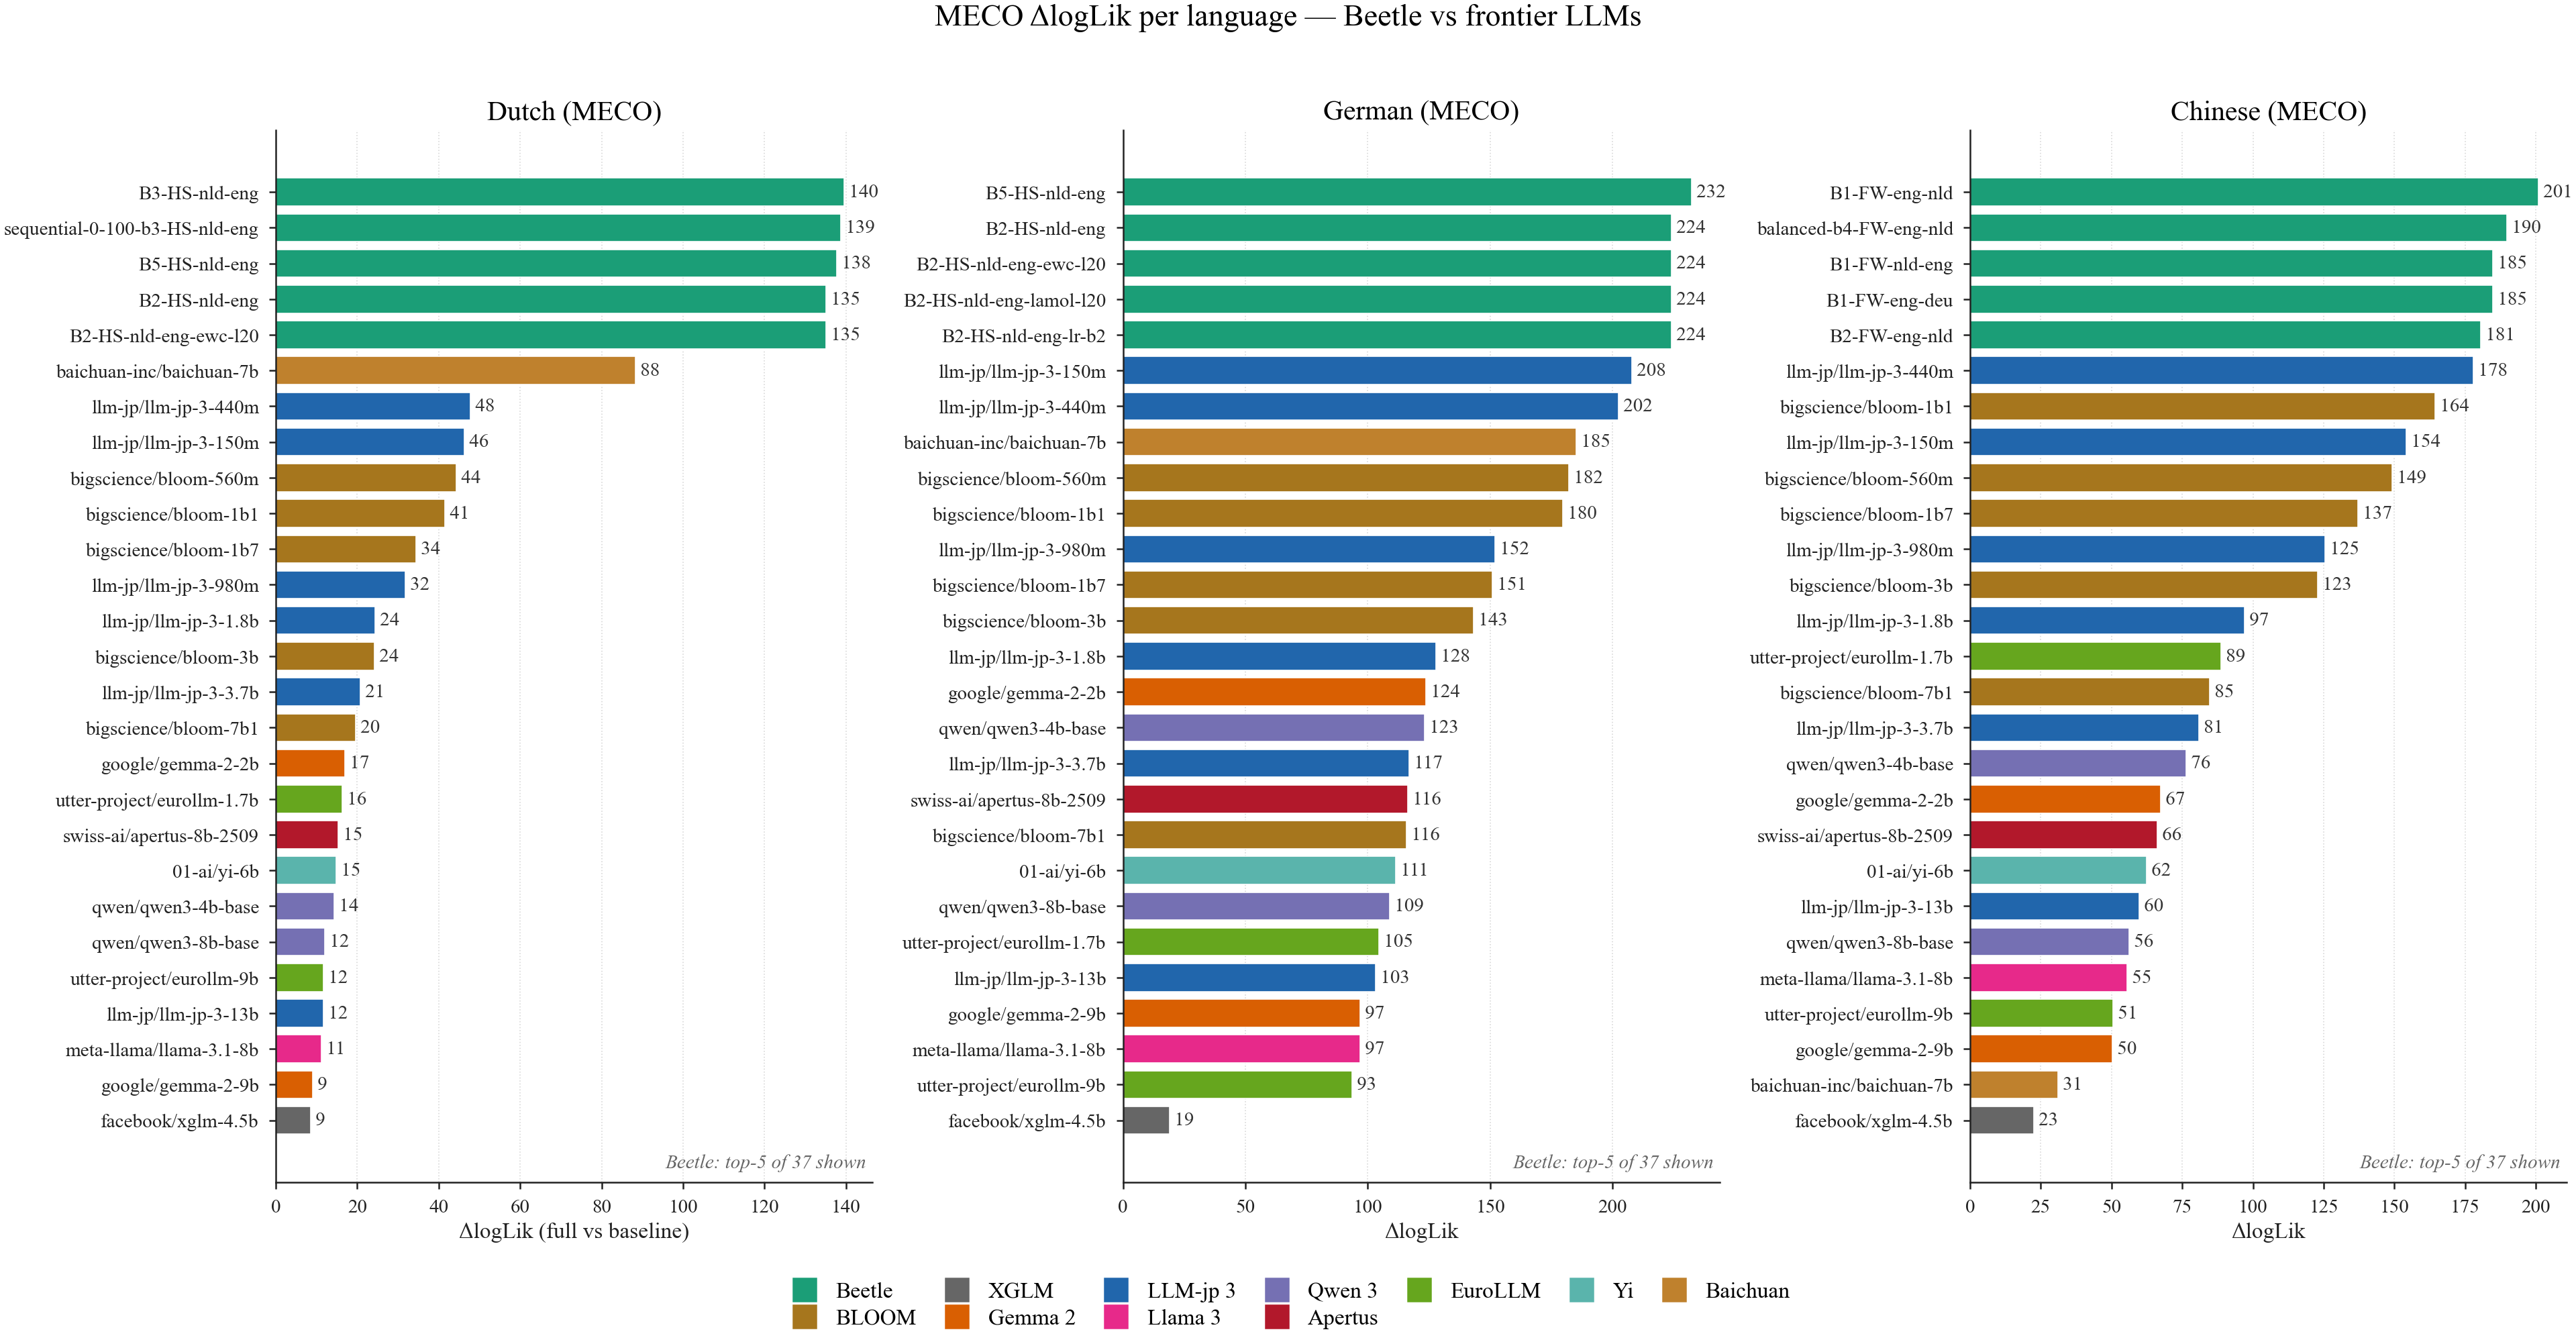
\includegraphics[width=1\linewidth]{fig/fig_meco_beetle_vs_baselines_bars.png}
    \caption{\textbf{MECO L2 $\Delta\log L$ per reader-L1 panel: Beetle vs.\ frontier LLMs.} Eight-panel grid, one panel per MECO~L2 reader-L1, with grouped horizontal bars for every model in the comparator set (Beetle B1--B5 monolingual and bilingual variants at 100\,M / 2\,B / 24\,B; modern bilingual LLMs Apertus-8B, EuroLLM-9B, XGLM-4.5B, Aya-tiny; legacy BLOOM-560m / 1b1 / 1b7 / 7b1). Per-panel ordering is by descending $\Delta\log L$. Headline: matched-bilingual Beetle bars cluster at the top of every Germanic-L1 panel; the modern bilingual LLM cohort trails the matched-bilingual Beetle on every panel including Chinese~L2.}
    \label{fig:meco_baselines_bars}
\end{figure}


\begin{figure}[!ht]
    \centering
    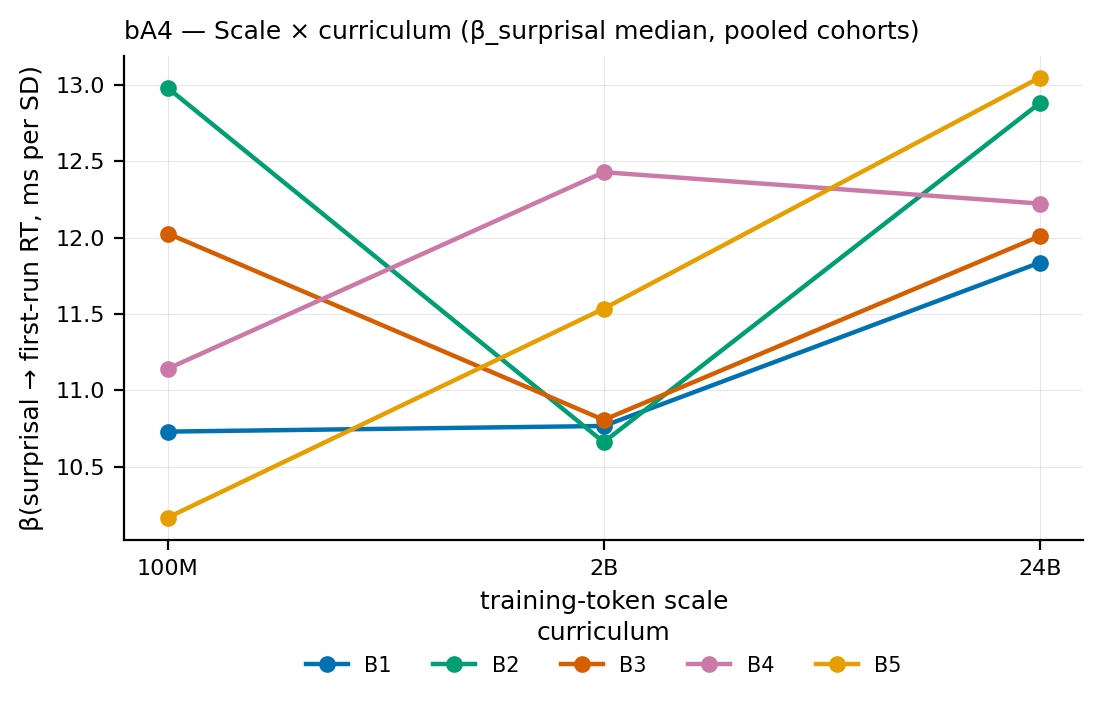
\includegraphics[width=1\linewidth]{fig/meco/bA4_scale_x_curriculum.png}
    \caption{\textbf{bA4 --- scale $\times$ curriculum on $\beta$-surprisal.} Median per-subject $\beta$(surprisal) random slope on MECO~L2 first-pass (first-run) duration, pooled across reader L1s, plotted against training-token cohort (HumanScale~100\,M / FineWeb~2\,B / FineWeb~24\,B) with one line per Beetle curriculum (B1--B5; nld--eng). Higher $\beta$ indicates stronger per-bit reading-time sensitivity. Headline: the curriculum ordering on $\beta$-surprisal is preserved across scale --- structured-exposure schedules (B2/B3-33/B5) dominate the balanced B1 schedule at every token budget.}
    \label{fig:bA4_scale_x_curriculum}
\end{figure}


\begin{figure}[!ht]
    \centering
    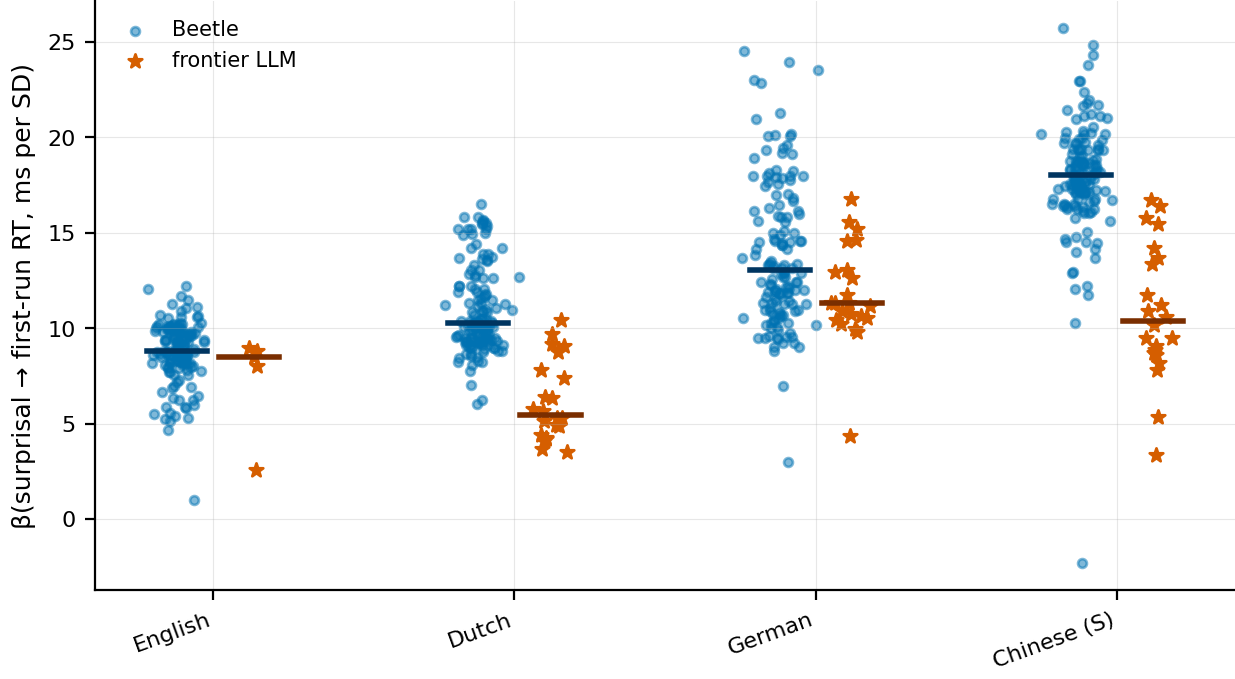
\includegraphics[width=1\linewidth]{fig/meco/bA5_beetle_vs_llm.png}
    \caption{\textbf{bA5 --- Beetle vs.\ frontier LLM on $\beta$-surprisal.} Per-curriculum $\beta$(surprisal) median for matched-bilingual Beetle 125\,M models (B1--B5; nld--eng, deu--eng, zho--eng) vs.\ four modern bilingual LLMs (Apertus-8B, EuroLLM-9B, XGLM-4.5B, Aya-tiny) on the same MECO~L2 reader-L1 cells. Higher $\beta$ indicates stronger psycholinguistic alignment per bit of surprisal. \emph{Note:} LLM bars use checkpoint-end values rather than training-time curves because public checkpoints are not log-spaced.}
    \label{fig:bA5_beetle_vs_llm}
\end{figure}



\begin{figure}[!ht]
    \centering
    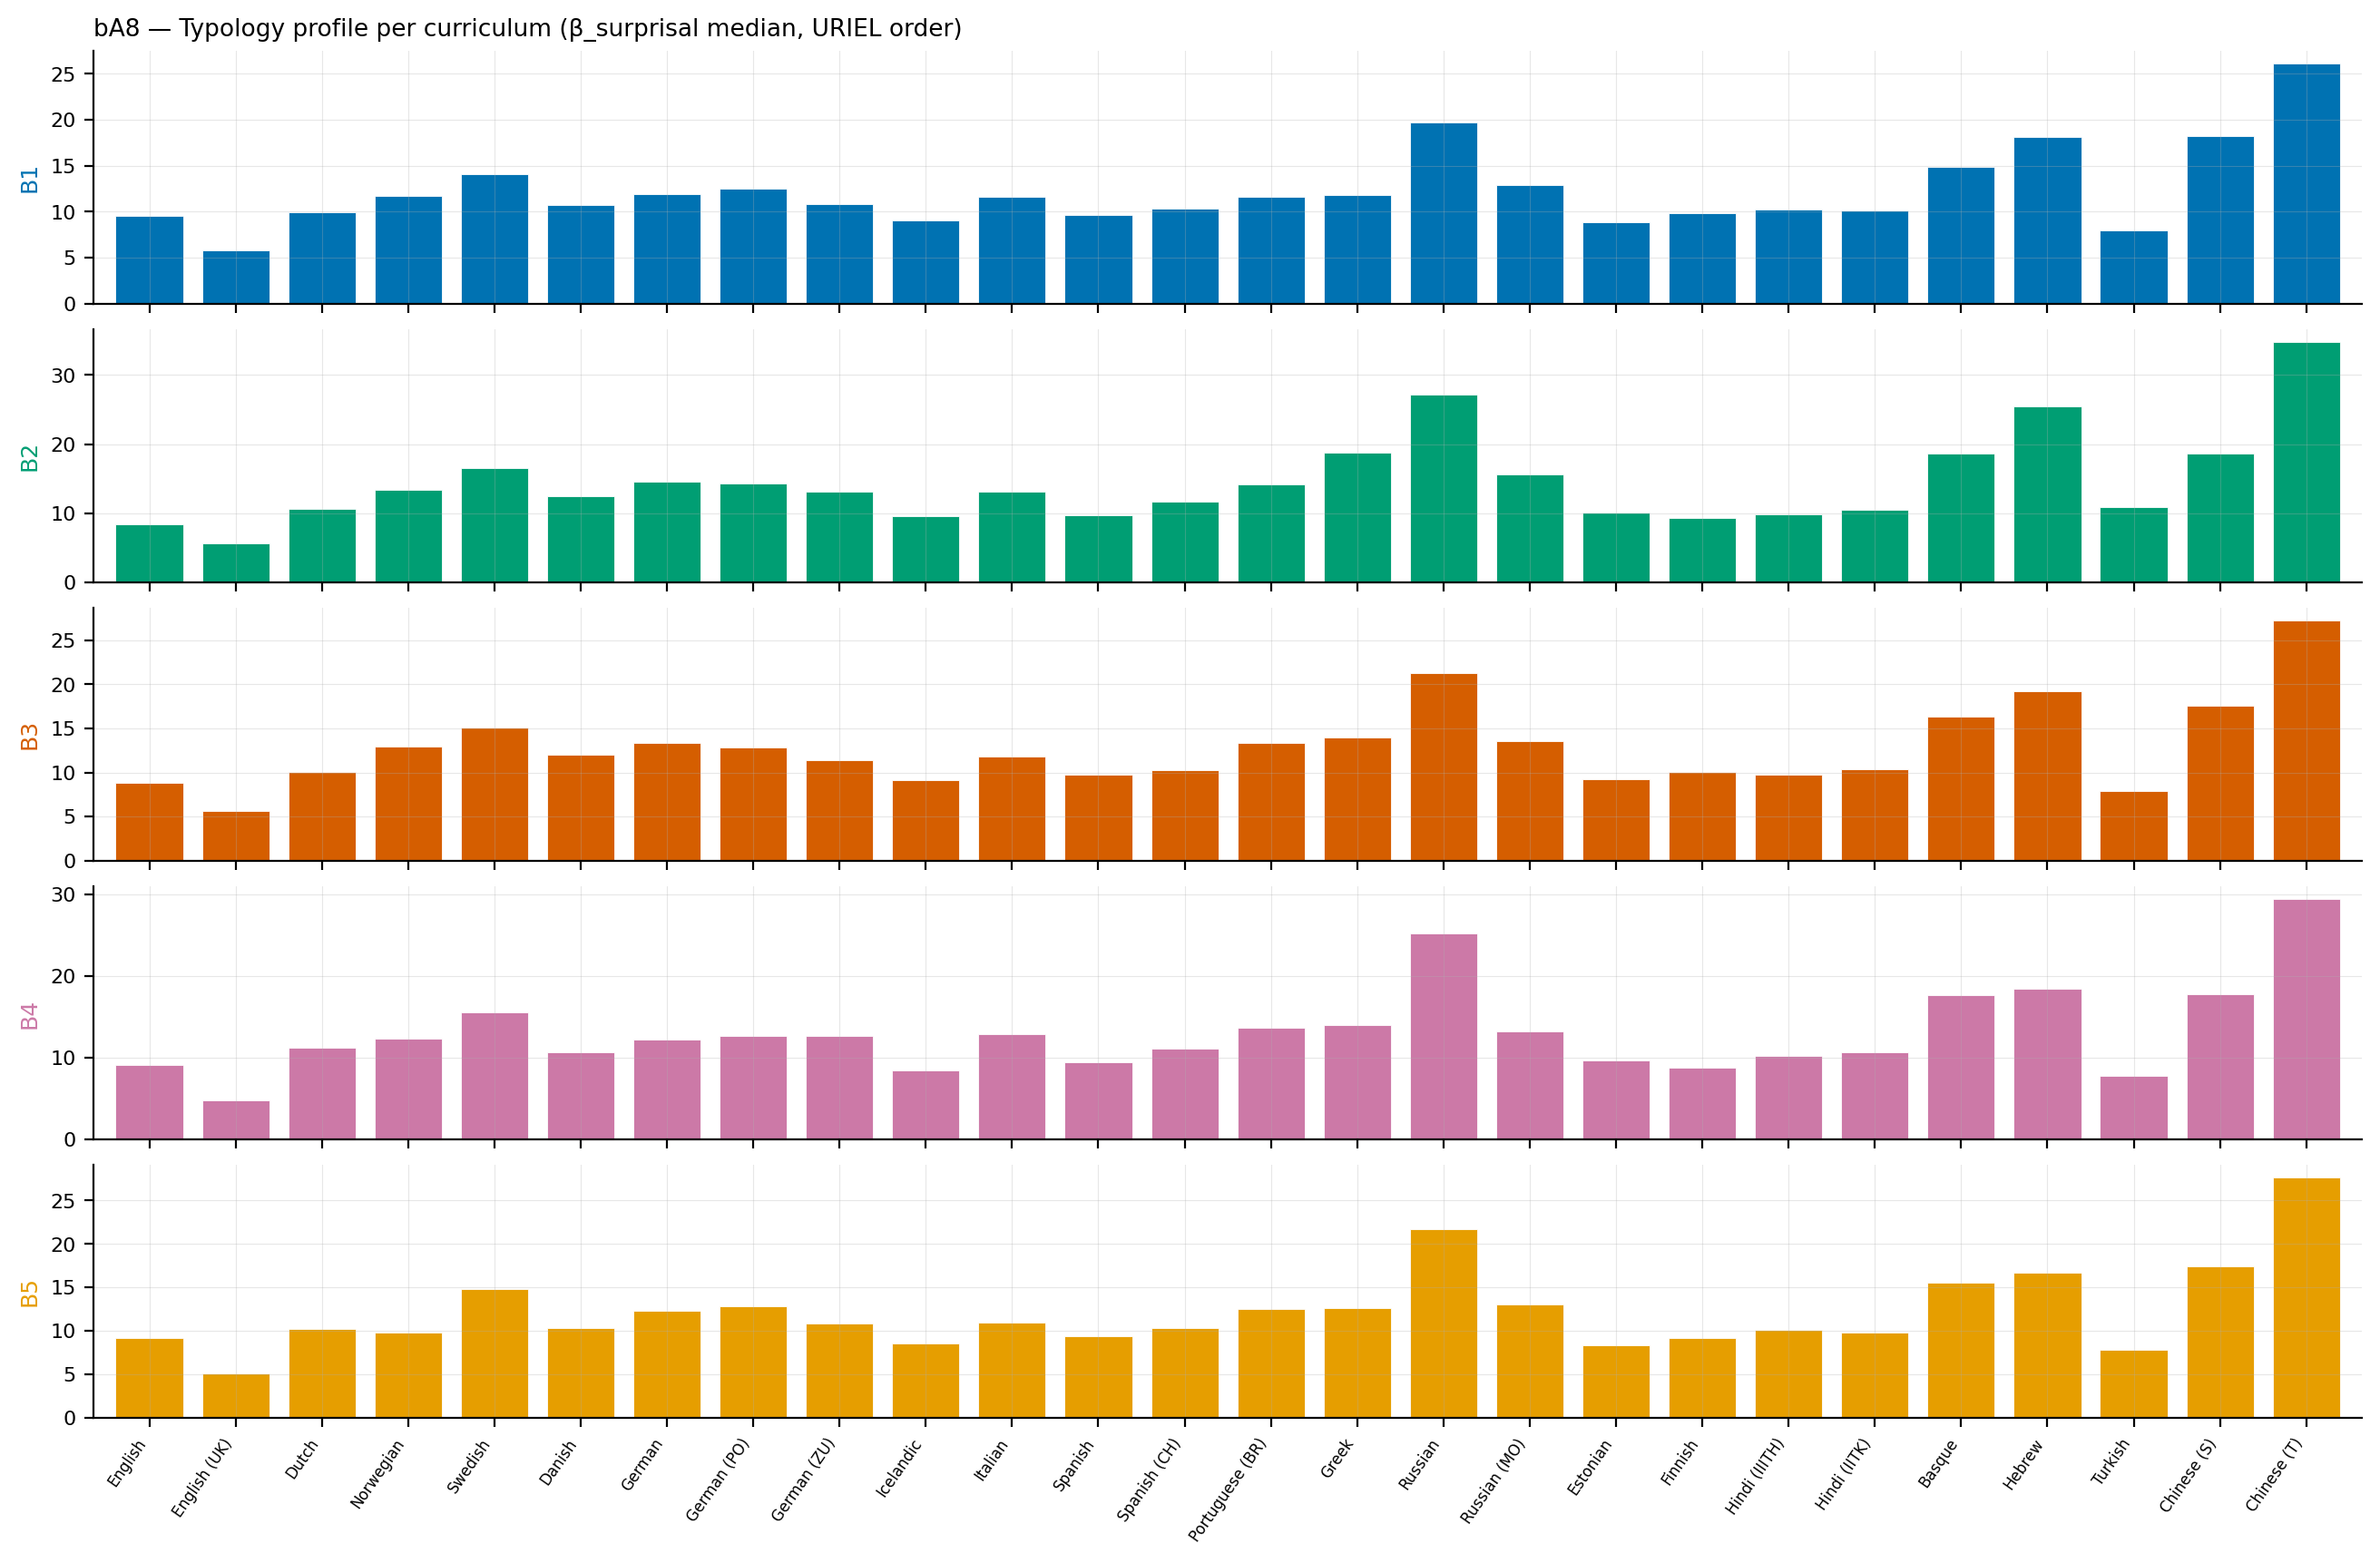
\includegraphics[width=1\linewidth]{fig/meco/bA8_typology_per_curriculum.png}
    \caption{\textbf{bA8 --- Typological-distance profile per curriculum.} Per-curriculum (B1--B5; one panel each) profile of MECO~L2 $\beta$(surprisal) across L1s ordered by linguistic distance from English (\textsc{nld} $<$ \textsc{deu} $<$ \textsc{spa} $<$ \textsc{rus} $<$ \textsc{fin/tur} $<$ \textsc{heb} $<$ \textsc{zho}; URIEL distance). The B3-33 / B5 advantage concentrates on the L1-proximate Germanic cell and attenuates monotonically as typological distance grows, replicating the typological-distance gradient seen on the $\Delta\log L$ axis (Fig.~\ref{fig:meco_curriculum}).}
    \label{fig:bA8_typology_per_curriculum}
\end{figure}

\begin{figure}[!ht]
    \centering
    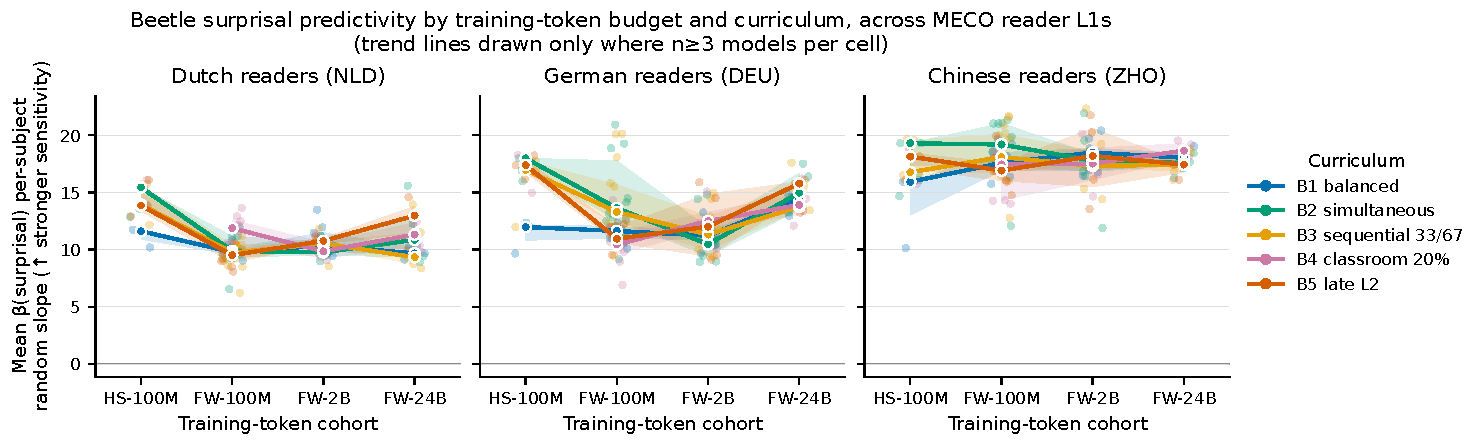
\includegraphics[width=1\linewidth]{fig/meco/fig1_scaling_x_curriculum.pdf}
    \caption{\textbf{Beetle surprisal predictivity by training-token budget $\times$ curriculum.} Mean $\beta$(surprisal) per-subject random slope (y-axis, $\uparrow$ stronger sensitivity) plotted against training-token cohort (x-axis: HumanScale~100\,M / FineWeb~2\,B / FineWeb~24\,B) for each Beetle curriculum (B1--B5; nld--eng, deu--eng). One panel per reader-L1 cohort. Headline: B3-33 and B5 sustain higher per-token psycholinguistic alignment than balanced B1 at every scale, and the gap widens with training tokens for Germanic L1s.}
    \label{fig:fig1_scaling_x_curriculum}
\end{figure}

\begin{figure}[!ht]
    \centering
    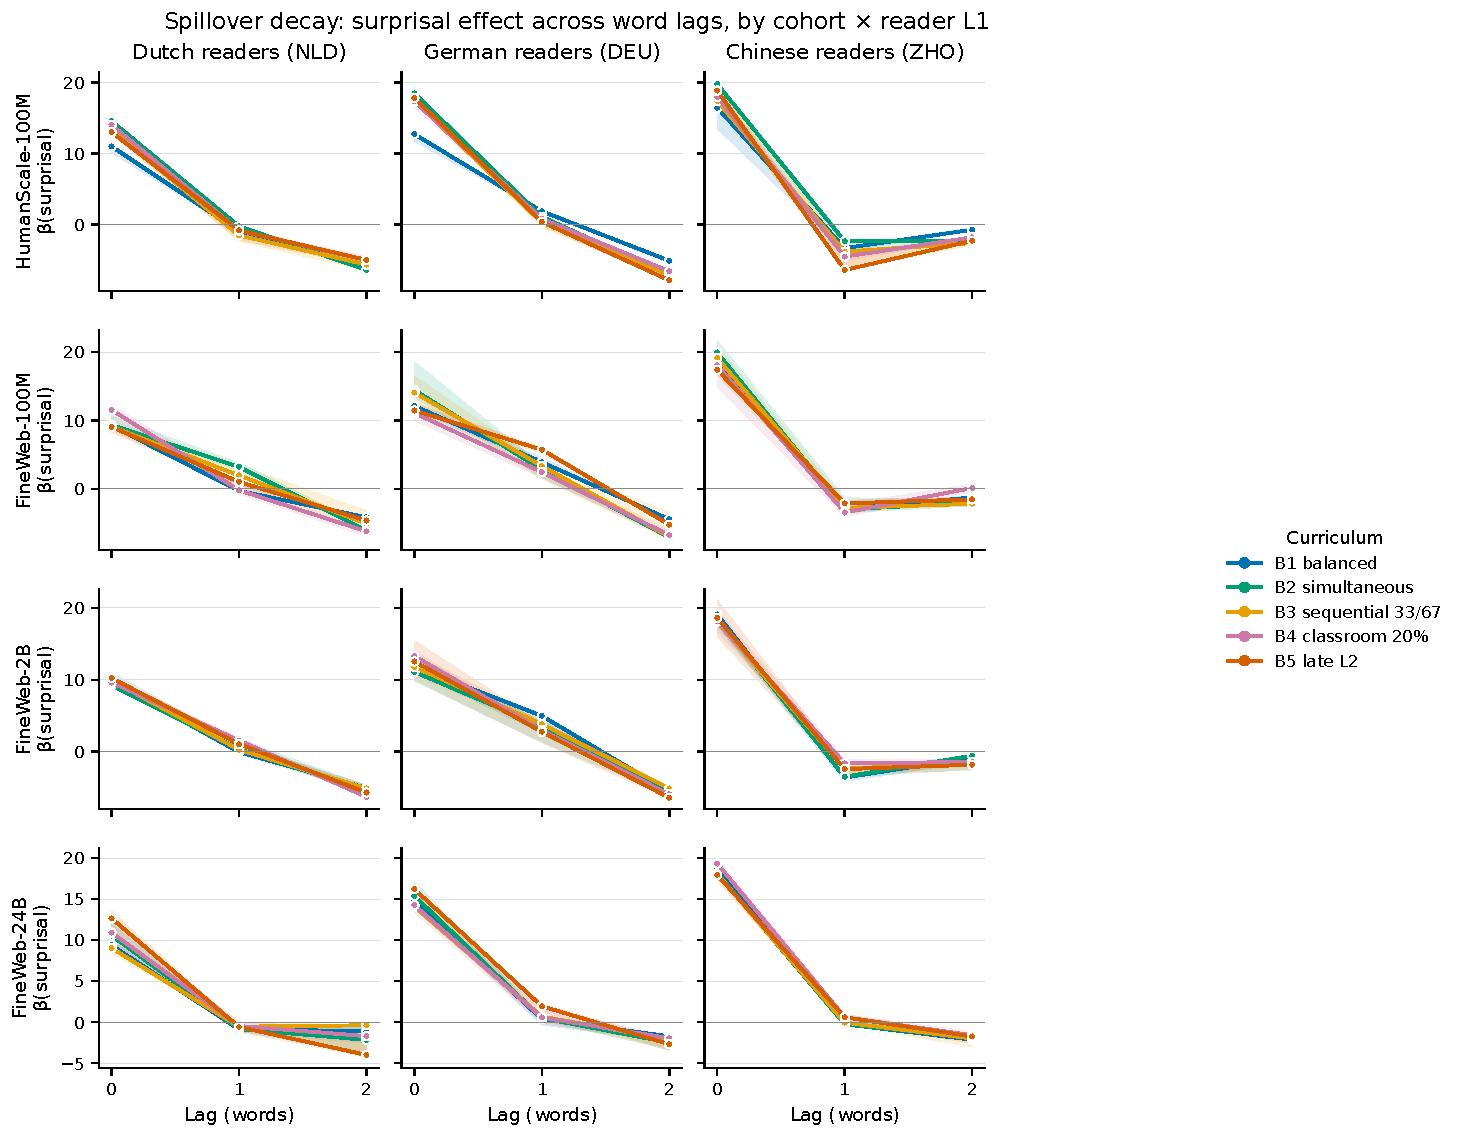
\includegraphics[width=1\linewidth]{fig/meco/fig3_spillover_decay.pdf}
    \caption{\textbf{Spillover decay: $\beta$(surprisal) across word lags by cohort $\times$ reader-L1.} For each (training-token cohort, reader-L1) cell, the panel plots the spillover $\beta$(surprisal) coefficient at lags 0--3 (x-axis = lag in words) on MECO~L2 first-pass (first-run) duration. Headline: staged curricula (B2/B3-33/B5) concentrate surprisal effect at lag~0 (early lexical access), whereas balanced B1 produces a flatter, lag-distributed profile (later integration). The lag-0 dominance grows with training tokens for Germanic L1s.}
    \label{fig:fig3_spillover_decay}
\end{figure}



\begin{figure}[!ht]
    \centering
    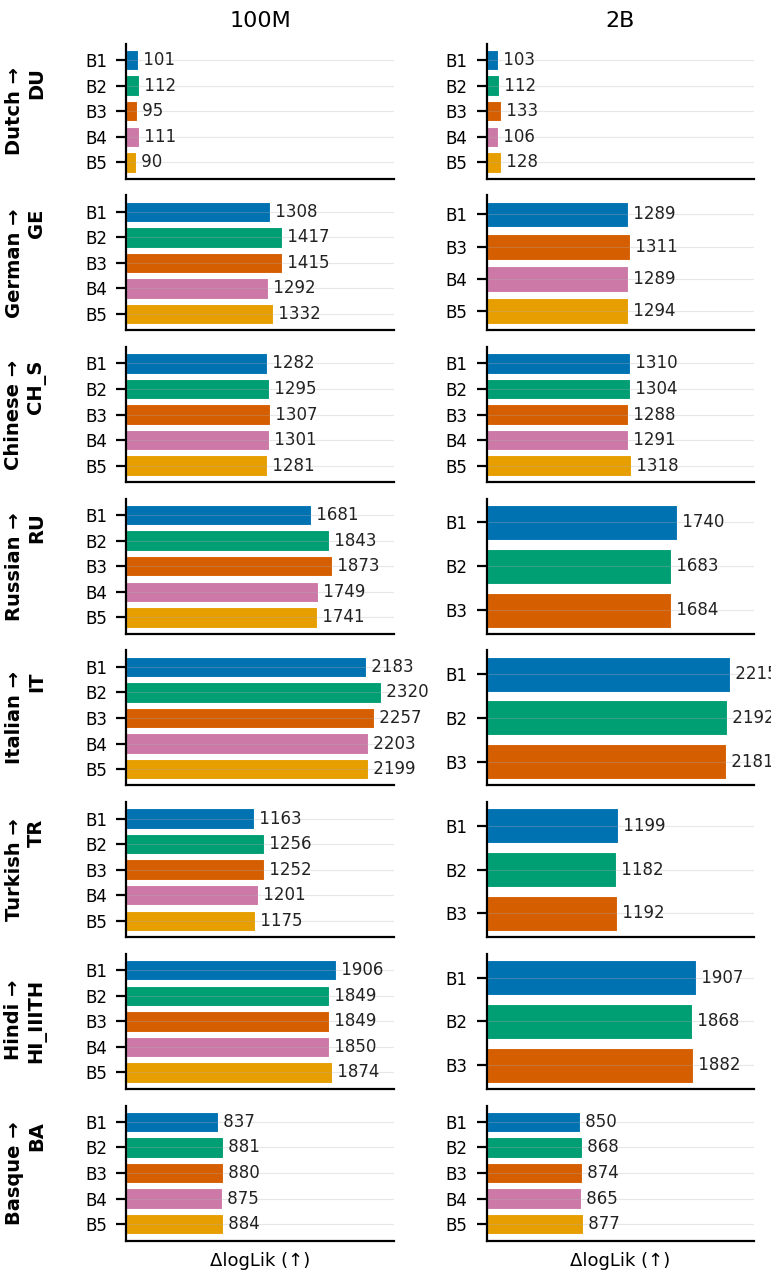
\includegraphics[width=0.8\linewidth]{fig/meco/fig9b_curriculum_sweep_matched.png}
    \caption{\textbf{F9b --- Curriculum effect on cognitive fit, L1-matched cohort, per training L1.} Grid of per-curriculum horizontal-bar panels (rows = training L1 \{nld, deu, zho, rus, fin, tur, heb, spa\}; cols = training-token scale \{100\,M, 2\,B, 24\,B, HS\}); each bar reports MECO~L2 mean $\Delta\log L$ on the matched-L1 reader cell. Empty cells indicate runs not yet trained. Headline: structured-exposure curricula (B3-33, B5) dominate the matched-L1 reader cell at every scale where the run exists, and the cross-curriculum spread is largest for Germanic L1s.}
    \label{fig:fig9b_curriculum_sweep_matched}
\end{figure}




\newpage 



\section{BLiSS Curriculum, Token Efficiency, and Metric Tradeoff}\label{sec:bliss-detail}

\subsection{BLiSS metric definitions}\label{sec:bliss-metric-defs}

\paragraph{Per-item normalised margin.} Let $\mathrm{BPT}(\cdot)$ denote bits-per-token. For each triplet (good, learner-error, artificial-error), define $\Delta_h = \mathrm{BPT}(\text{learner}) - \mathrm{BPT}(\text{good})$ and $\Delta_r = \mathrm{BPT}(\text{artificial}) - \mathrm{BPT}(\text{good})$. The normalised gap is $\mathrm{gap} = (\mathrm{BPT}(\text{artificial}) - \mathrm{BPT}(\text{learner}))/(|\Delta_r| + |\Delta_h| + \varepsilon)$.

\paragraph{Normalised Gap Score (NGS).} Aggregating across items, $\mathrm{NGS} = 100\times(0.5 + 0.5\cdot\mathbb{E}[\mathrm{gap}])$. Chance performance is 50.

\paragraph{Correct-Preferred Sanity (CPS).} The fraction of triplets where the correct sentence is assigned the lowest BPT: $\mathrm{CPS} = 100\times N^{-1}\sum_i \mathbb{I}[\mathrm{BPT}(\text{good}_i) < \min(\mathrm{BPT}(\text{learner}_i), \mathrm{BPT}(\text{artificial}_i))]$. CPS is a binary sanity check (does the model rank the correct sentence first?); NGS is a continuous, margin-based metric.

\paragraph{Random-over-human Preference (RP$@\tau$).} The fraction of items where $\mathrm{BPT}(\text{artificial}) > \mathrm{BPT}(\text{learner}) + \tau$. RP$@0$ is the strict zero-margin version (the headline number reported in \S\ref{sec:discrim-bliss}). Higher values indicate the model finds artificial perturbations more surprising than human learner errors --- the desired pattern.

\begin{table*}[!ht]
  \centering
  \small
  \caption{\textbf{BLiSS RP$@0$ by exposure curriculum $\times$ training scale $\times$ L1.} 95\% Wilson CIs in brackets. Source: \texttt{plots/fig\_bliss\_main\_curriculum.csv}. RP$@0$ is the random-over-human preference rate at zero margin; chance = 50; higher is better for matched-L1 cells. Bold = best in row. The body BLiSS curriculum conclusions rest on the nld--eng FineWeb cells; the deu--eng row caveat is in the paragraph immediately following the table.}
  \label{tab:bliss_canonical}
  \begin{tabular}{llrrrrr}
    \toprule
    L1$\to$L2 & Scale & B1 & B2 & B3-33 & B4 & B5 \\
    \midrule
    nld$\to$eng & HumanScale & 56.64 & 57.55 & \textbf{57.66} & 57.32 & 57.09 \\
    nld$\to$eng & FineWeb    & 56.64 & 60.05 & \textbf{62.09} & 58.57 & 60.27 \\
    deu$\to$eng & HumanScale & 57.17 & 54.83 & \textbf{55.48} & 54.75 & 55.23 \\
    deu$\to$eng & FineWeb    & 53.14 & 54.91 & --- & 54.67 & \textbf{58.29} \\
    zho$\to$eng & HumanScale & 63.21 & 63.75 & 63.97 & 60.42 & \textbf{64.25} \\
    \bottomrule
  \end{tabular}
\end{table*}

\paragraph{Caveat: deu--eng HumanScale row.} The deu--eng HumanScale row sits 5--7 points above chance ($\sim$53--57); at one seed and that proximity to chance the within-row B1$>$B3-33 ordering is within noise. We therefore do not read curriculum conclusions off the deu--eng HumanScale BLiSS row; the body BLiSS curriculum-by-task conclusions (\S\ref{sec:discrim-bliss}) rest on the nld--eng FineWeb cells where the spread is $\sim$5--6 points.

\subsection{BLiSS figure set}

\begin{figure}[!ht]
  \centering
  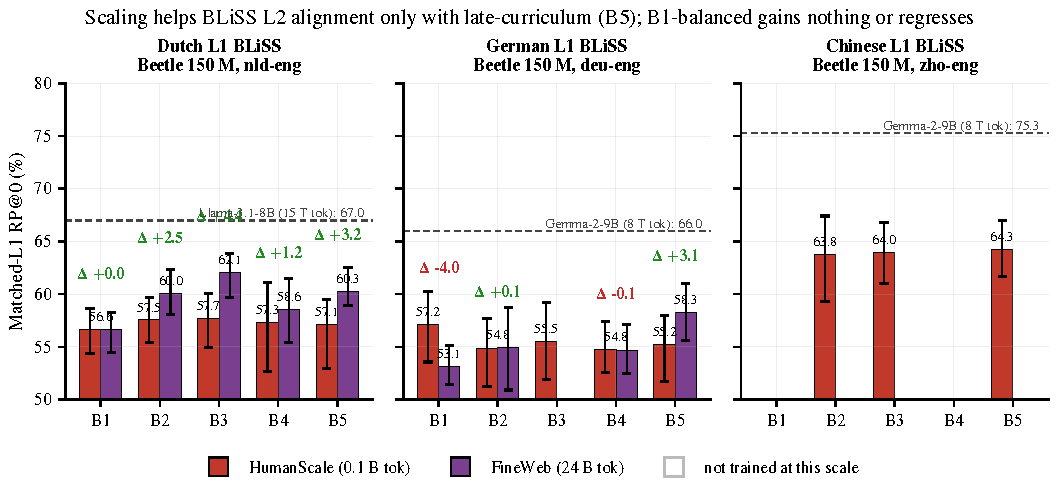
\includegraphics[width=\linewidth]{fig/F7_bliss_curriculum_x_scale.pdf}
  \caption{BLiSS NGS by exposure curriculum (B1--B5) $\times$ training scale (\textsc{HumanScale}~100M, \textsc{FineWeb}~2B). Unlike MECO, simultaneous (B2) and balanced (B1) schedules dominate at FineWeb scale; late-onset B5 is competitive at HumanScale. BLOOM and XGLM baselines are shown; \textsc{Beetle} FineWeb models surpass the BLOOM-7b1 NGS at both scales.}
  \label{fig:bliss_curriculum_scale}
\end{figure}

\begin{figure}[!ht]
  \centering
  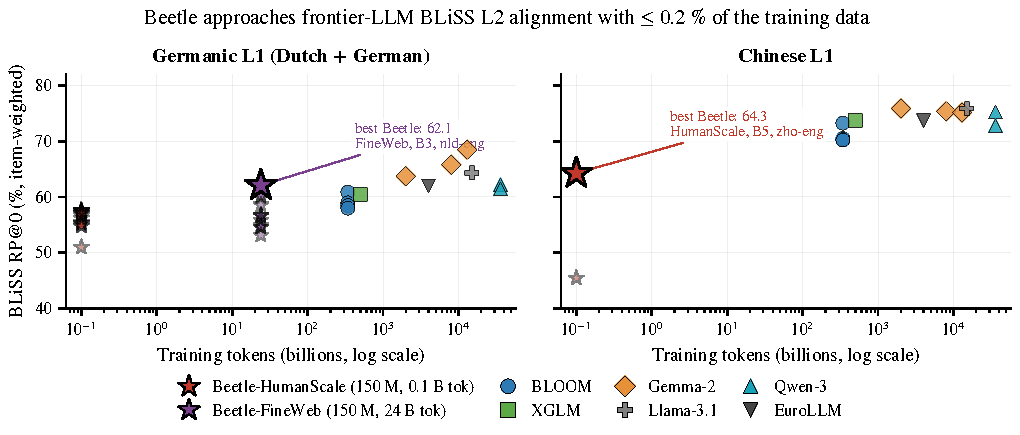
\includegraphics[width=\linewidth]{fig/F6_bliss_token_efficiency.pdf}
  \caption{BLiSS NGS as a function of training tokens for \textsc{Beetle} models (nld--eng, B1--B5) vs.\ baselines. Simultaneous B2 and balanced B1 reach competitive NGS earlier than sequential / late schedules --- the \emph{reverse} of the MECO token-efficiency ordering (Fig.~\ref{fig:meco_efficiency}).}
  \label{fig:bliss_efficiency}
\end{figure}

\begin{figure}[!ht]
  \centering
  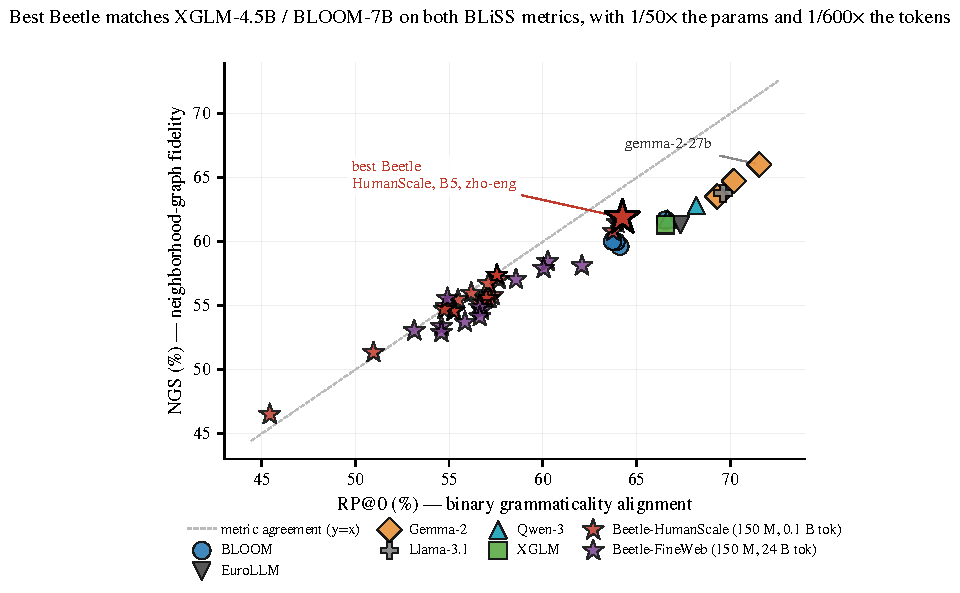
\includegraphics[width=\linewidth]{fig/F8_bliss_metric_tradeoff_pareto.pdf}
  \caption{BLiSS metric tradeoff: NGS vs.\ CPS vs.\ RP$@\tau$ across \textsc{Beetle} curricula and baselines. Among matched-L1 \beetle{} cells, B5 zho--eng HumanScale leads on RP$@0$ ($\textbf{64.25}$) and NGS ($\textbf{61.88}$); B3-33 nld--eng FineWeb is the matched-Germanic leader (RP$@0 = 62.09$, NGS $= 58.11$); B1 nld--eng FineWeb leads matched-L1 CPS at $56.75$. The multilingual-LLM cohort exceeds the \beetle{} per-cell maximum on RP$@0$ (Gemma-2, Llama-3.1, Qwen-3 reach $\sim$66--71 on the pooled-L1 evaluation), so the leadership claim is within-\beetle{} only. Source: \texttt{results/evals\_checkpoints/bliss/bliss\_results.csv}, branch \texttt{main}, item-weighted; the per-(L1, scale, curriculum) Wilson-CI cells are Tab.~\ref{tab:bliss_canonical}. Earlier-draft headline values of $64.9 / 68.5$ were generated by a deprecated pipeline and have been retired.}
  \label{fig:bliss_pareto}
\end{figure}


\newpage
\section{Pedagogical Utility and CEFR Stratification}\label{sec:pedagogical-detail}

\paragraph{CEFR-perplexity gradient and CEFR-stratified BLiSS (deferred from body).} The matched mono-eng anchor shows an L1-like CEFR-perplexity gradient of $+3.26$ bits from A1$\to$C2 (Tab.~\ref{tab:headline_pedagogical}, A1$\to$C2 grad.\ column); the bilingual nld--eng curricula show shallower $+2.0$--$2.25$-bit gradients (B1 HS = 2.247; B5 HS = 2.066), consistent with expectations for L2 readers. CEFR-stratified BLiSS RP$@0$ under matched-L1 conditions shows the single-seed curriculum-by-difficulty cells reported in Tab.~\ref{tab:headline_pedagogical} (and in the released analysis bundle); e.g.\ B2 simultaneous peaks at A2, B4 classroom peaks at B1, mono-eng dominates C1. We report these as single-seed cell readings consistent with a learner-difficulty profile rather than as tested learner-difficulty claims; the body pedagogical claim rests on the CLOTH and JFLEG anchors of \S\ref{sec:discrim-cefr}.

 This appendix supports the three body pedagogical readouts of \S\ref{sec:discrim-cefr} and the demoted CUP\&A5 diagnostic. The per-model values in Tab.~\ref{tab:headline_pedagogical} back the body claims that the matched-bilingual nld--eng \beetle{} recovers the monolingual-English anchor to within $0.01$ on CLOTH and to within $0.06$ bits/token on JFLEG. The pedagogical-utility ladder of Fig.~\ref{fig:ped_ladder} places \beetle{} on the same axis as the GPT-3.5 / GPT-4 references of \citet{benedetto-etal-2024-using} so the 125M parameter-scale ceiling on RC-MCQ is visible. The CEFR-stratified RC-MCQ figure (Fig.~\ref{fig:rcmcq_cefr}) and the moved CUP\&A5 monotonicity diagnostic (\S\ref{sec:cupa5-monotonicity-appendix}) together support the body assertion that no \beetle{} model produces a CEFR-inverted profile (so the diagnostic doesn't \emph{fail}), while making explicit that the absolute accuracy is too low for the monotonicity to be a competence claim.

\begin{table*}[!ht]
  \centering
  \scriptsize
  \setlength{\tabcolsep}{4pt}
  \caption{\textbf{Pedagogical readouts per \beetle{} model.} CLOTH closed-cloze accuracy, Cambridge open-cloze accuracy, JFLEG learner-fluency margin (bits/token; positive = model prefers corrected over learner-error sentence), false-friend disambiguation margin (bits/token), CEFR-A1 / CEFR-C2 BPT and CEFR gradient (bits between A1 and C2 perplexity). Source: \texttt{plots/headline\_summary\_table.csv}. Bold = best per column within the matched-L1 nld--eng family.}
  \label{tab:headline_pedagogical}
  \begin{tabular}{llrrrrrrr}
    \toprule
    Model & Family & CLOTH & Camb.~OC & JFLEG (bits) & FF (bits) & A1 BPT & C2 BPT & A1$\to$C2 grad. \\
    \midrule
    B1 nld--eng     & HS & \textbf{0.380} & \textbf{0.644} & \textbf{0.949} & \textbf{0.585} & 6.572 & 8.818 & 2.247 \\
    B2 nld--eng     & HS & 0.302 & 0.596 & 0.750 & 0.156 & 8.051 & 10.213 & 2.163 \\
    B3-33 nld--eng  & HS & 0.310 & 0.587 & 0.751 & 0.174 & 8.106 & 10.275 & 2.169 \\
    B4 nld--eng     & HS & 0.304 & 0.582 & 0.801 & $-$0.055 & 7.719 & 9.755 & 2.036 \\
    B5 nld--eng     & HS & 0.302 & 0.584 & 0.716 & 0.238 & 8.127 & 10.193 & 2.066 \\
    \midrule
    B1 nld--eng     & FW-2B & 0.369 & 0.638 & 0.833 & 0.457 & 8.851 & 8.614 & $-$0.237 \\
    B2 nld--eng     & FW-2B & 0.322 & 0.567 & 0.502 & 0.238 & 10.317 & 11.047 & 0.730 \\
    B3-33 nld--eng  & FW-2B & 0.329 & 0.614 & 0.511 & 0.235 & 10.354 & 11.056 & 0.702 \\
    B4 nld--eng     & FW-2B & 0.325 & 0.602 & 0.562 & 0.256 & 10.143 & 10.730 & 0.587 \\
    B5 nld--eng     & FW-2B & 0.323 & 0.570 & 0.509 & 0.318 & 10.364 & 11.040 & 0.676 \\
    \midrule
    mono-eng        & HS & 0.369 & 0.659 & 0.888 & 0.351 & 7.297 & 10.558 & \textbf{3.261} \\
    mono-nld        & HS & 0.267 & 0.310 & 0.306 & $-$0.034 & 9.875 & 10.671 & 0.796 \\
    \bottomrule
  \end{tabular}
\end{table*}

\begin{figure*}[!ht]
  \centering
  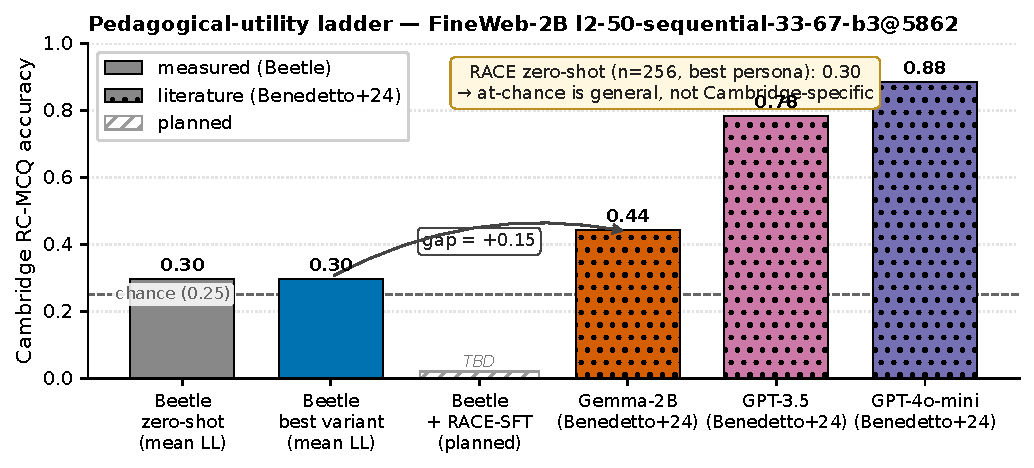
\includegraphics[width=\linewidth]{fig/P3_pedagogical_utility_ladder.pdf}
  \caption{\textbf{Pedagogical-utility ladder.} Cambridge CUP\&A5 RC-MCQ accuracy: Beetle zero-shot vs.\ Beetle best variant vs.\ Gemma-2B / GPT-3.5 / GPT-4o-mini reference rows from \citet{benedetto-etal-2024-using}. The Beetle-RACE-SFT bar is reserved (App.~\ref{sec:roadmap}, item~4) and rendered as a hatched placeholder. \emph{Licence and reproducibility.} The CUP\&A5 200-MCQA $\times$ 4-CEFR battery \citep{mullooly2023cupa5} is held under a Cambridge University Press \& Assessment internal licence and is \emph{not} part of the \beetle{} artefact release (see \S\ref{sec:reproducibility}); the body's pedagogical-axis headline claims (BLiSS, CLOTH, JFLEG) all rest on public resources, and this ladder is presented as the demoted RC-MCQ scale-ceiling diagnostic (\S\ref{sec:cupa5-monotonicity-appendix}), not as a load-bearing pedagogical claim. A public-only re-render of this ladder using RACE \citep{lai-etal-2017-race} as the CEFR-stratified MCQ axis is queued for the camera-ready (App.~\ref{sec:roadmap} item~4); at that point the CUP\&A5 panel will either be replaced by the RACE variant or retained alongside it with the CUP\&A5 columns explicitly marked as an internal-licence cell. Researchers wishing to reproduce the CUP\&A5 cells should obtain the battery from the original Cambridge authors.}
  \label{fig:ped_ladder}
\end{figure*}

\begin{figure*}[!ht]
  \centering
  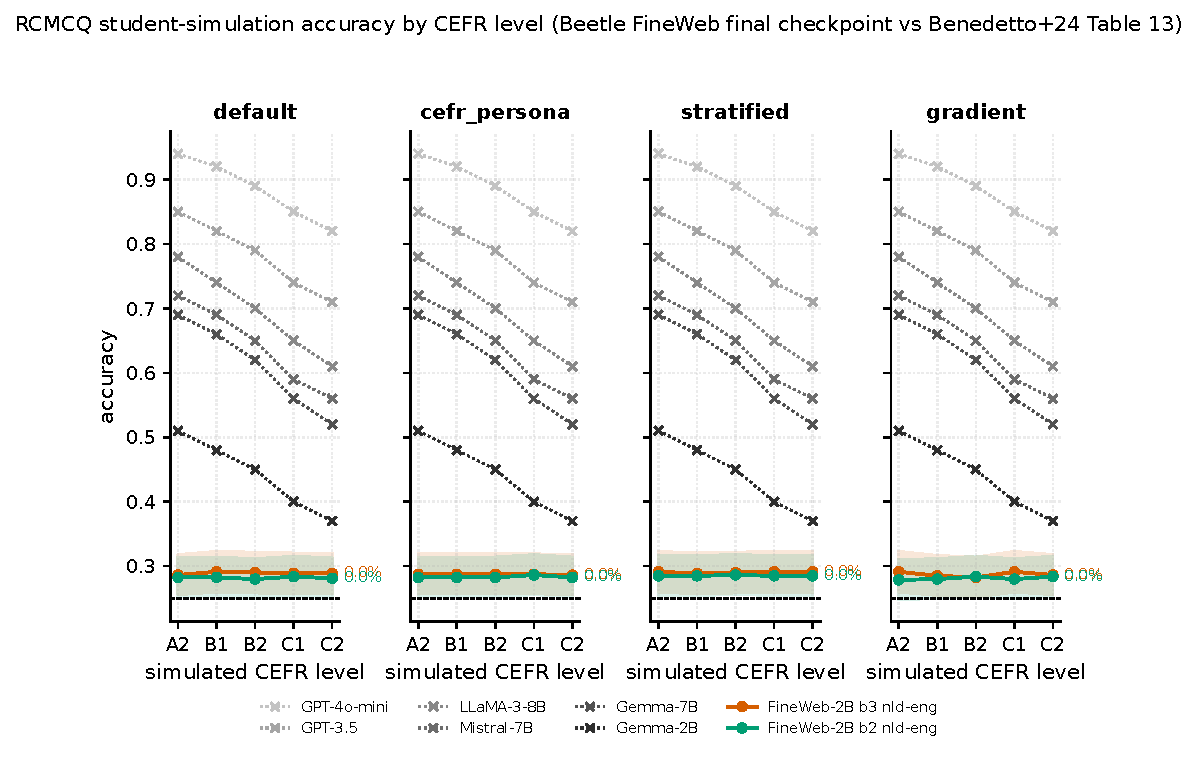
\includegraphics[width=\linewidth]{fig/P5_rcmcq_cefr.pdf}
  \caption{\textbf{CEFR stratification.} CEFR-stratified RC-MCQ accuracy under four prompting variants: \textsc{Beetle} FineWeb-2B B2/B3 vs.\ the six LLM rows of \citet{benedetto-etal-2024-using}. Beetle exhibits CEFR-monotonic behaviour on a subset of prompting variants.}
  \label{fig:rcmcq_cefr}
\end{figure*}

\subsection{CUP\&A5 Benedetto-monotonicity diagnostic}\label{sec:cupa5-monotonicity-appendix}

Every \beetle{} model satisfies $P=0$ on the Benedetto monotonicity score, i.e.\ per-CEFR-level RC-MCQ accuracy is monotone in difficulty. We do \emph{not} read this as a competence claim, because absolute RC-MCQ accuracy is 27.9--36.7\% (vs.\ 20\% four-choice chance), and monotonicity at near-chance accuracy is statistically near-trivial: item-difficulty curves shaped by item content alone can produce monotonic per-level scores at chance. We retain the diagnostic here to flag that no \beetle{} model produces a CEFR-inverted profile; the body's CEFR competence claim rests on the CEFR-perplexity gradient and the CEFR-stratified BLiSS RP$@0$ (\S\ref{sec:discrim-cefr}), not on RC-MCQ monotonicity.

\section{FLORES-200 Convergence Detail}\label{sec:flores-detail}

\begin{figure*}[!ht]
  \centering
  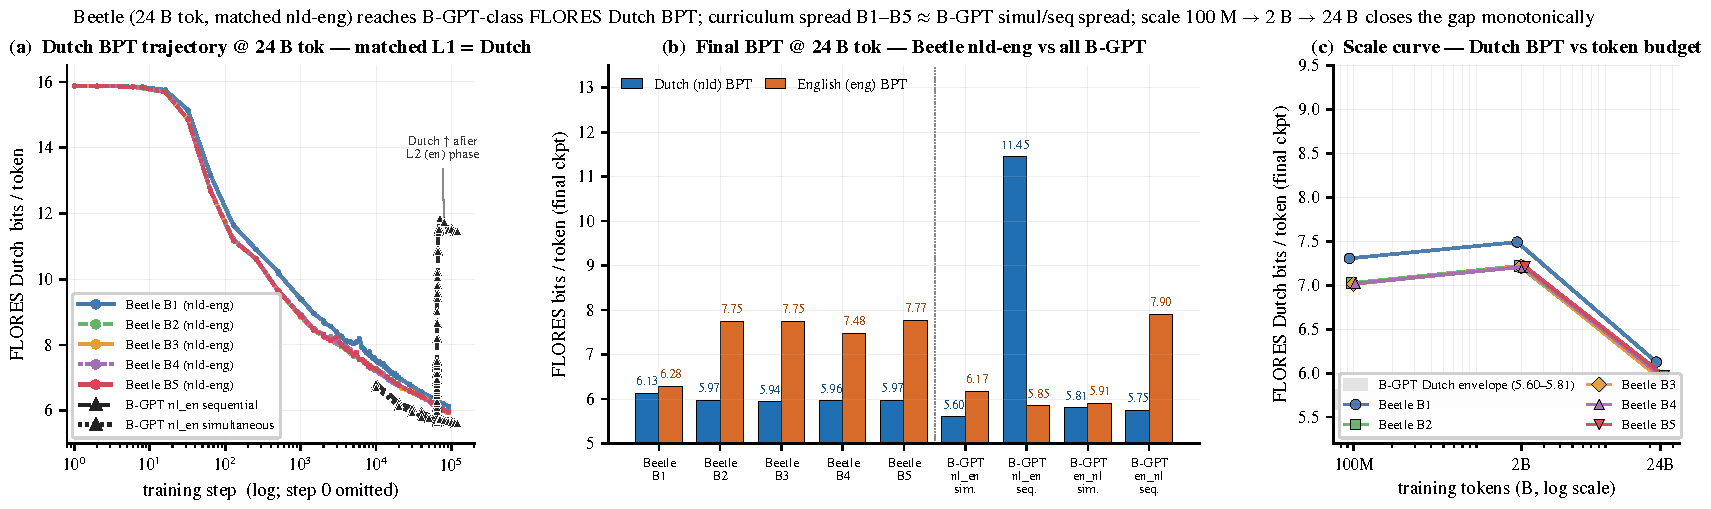
\includegraphics[width=\linewidth]{fig/F10_flores_beetle_vs_bgpt.pdf}
  \caption{\textbf{Bits-per-byte FLORES, Beetle vs.\ B-GPT (matched nld--eng).} (a) Dutch FLORES BPB trajectory across log-spaced \textsc{Beetle} training steps for the FineWeb-24B nld--eng cohort (B1--B5); the B-GPT non-forgetting envelope is drawn as a horizontal band because B-GPT checkpoints are not log-spaced. (b) Final-checkpoint Dutch / English FLORES paired bars at 24~B tokens for \textsc{Beetle} B1--B5 plus all four B-GPT variants. (c) Scale curve: final Dutch BPB versus 100~M / 2~B / 24~B token budget per curriculum, with the B-GPT non-forgetting envelope shaded. The matched-bilingual \textsc{Beetle} converges into the B-GPT band as the token budget grows; only the B-GPT \textsc{nl-en} sequential variant exhibits Dutch catastrophic forgetting (11.45 BPT).}
  \label{fig:flores_beetle_vs_bgpt}
\end{figure*}



\section{\beetle{} Control Parameters}\label{sec:beetle-control-parameters}

\paragraph{Exposure Schedules} For bilingual and trilingual experiments, language mixing is governed by one of six \emph{curriculum schedules} that modulate the per-step proportion of L1, L2, and (for trilingual runs) L3 tokens. The schedules --- \textbf{balanced}, \textbf{late}, \textbf{sequential}, \textbf{heritage}, \textbf{part\_time}, and \textbf{simultaneous} --- summarised in App.~\ref{sec:beetle-curricula} span the space from fully interleaved exposure (modelling balanced bilingual/trilingual acquisition) to sequential exposure (modelling a more extreme acquisition scenario where learners receive no L1 input upon the acquisition of L2 in a bilingual setting, or no L1 and L2 input upon the acquisition of L3).

\subsection{Control Parameters}

All continual-learning experiments fix the language order to English~$\to$~Dutch~$\to$~Chinese under a uniform trilingual \texttt{sequential} exposure schedule, using the same PicoDecoder architecture and training budget as the main sweep ($T_{\max}\!=\!30{,}578$ steps). For EWC, we vary the regularisation strength $\lambda\!\in\!\{5,\,20,\,50,\,150\}$; the values $\lambda\!=\!20$ and $\lambda\!=\!150$ replicate settings reported in \citep{constantinescu2025investigating}.  The Fisher diagonal $\hat{F}$ is estimated on $K\!=\!10$ held-out L1 batches at the L1$\to$L2 phase boundary, and the anchor parameters~$\theta^*$ are snapshotted at the same moment; the penalty is then active for the remainder of training. For MAML, we vary the hybrid ratio $r\!\in\!\{0.25,\,0.50,\,0.75,\,1.00\}$, which controls the fraction of training steps executed as $N$-way, $K$-shot meta episodes ($N\!=\!5$, $K\!=\!1$, 3 inner SGD steps at $\alpha\!=\!0.1$) versus standard autoregressive steps. We have a combined condition that combines all four EWC strengths with all four hybrid ratios, yielding a $4\!\times\!4$ factorial design, which we compare against a trilingual baseline, producing 25 experimental conditions, each trained and evaluated identically to the baseline trilingual run.

%\paragraph{Multilingual Data Quality} We use FineWeb2 \citep{penedo2025fineweb2} for 2B tokens of bilingual model pretraining for the following languages: English, Japanese, Chinese, French, German, (Italian), Basque, Turkish, Indonesian. We do data decontamination.  \textit{ignore for potential CDL submission}


\subsection{Meta-Learning}

\beetle{}  uses the \texttt{pico-maml} implementation of MAML used in \citet{africa-etal-2025-learning} and \citet{africa-etal-2025-meta}. 


\begin{algorithm}\small \caption{Distributed SMLMT Loop}\label{alg:dist-maml} \begin{algorithmic} \State Initialize model $f_\theta$, head $h_\phi$, outer optimizer, and inner SGD on $h_\phi$ \State step $\leftarrow 0$ \For{each sub-batch $B$ from dataloader} \State $X \leftarrow \text{AllGather}(B\ \text{inputs})$ \Comment{across devices} \State $r \leftarrow \text{Broadcast}(\text{Uniform}(0,1))$ \If{$r < \rho$} \State $(S,Q,y_S,y_Q) \leftarrow \text{MaskTokens}(X)$ \State $\phi_{\text{snap}} \leftarrow \phi$ \Comment{save head params} \For{$t = 1$ to $T_{\text{inner}}$} \State $\ell_S \leftarrow \text{CE}\big(h_\phi(f_\theta(S)),,y_S\big)$ \State $\phi \leftarrow \phi - \alpha,\nabla_\phi \ell_S$ \EndFor \State $\ell \leftarrow \text{CE}\big(h_\phi(f_\theta(Q)),,y_Q\big)$ \State $\phi \leftarrow \phi_{\text{snap}}$ \Comment{restore head} \Else \State $X_{\text{in}} \leftarrow X$ without last token; $Y \leftarrow X$ without first token \State $\ell \leftarrow \text{CE}\big(f_\theta(X_{\text{in}}),,Y\big)$ \EndIf \State Backward$\big(\ell ,/, \text{accum\_steps}\big)$ \If{$( \text{step} + 1 ) \bmod \text{accum\_steps} = 0$} \State OptimizerStep(); SchedulerStep(); ZeroGrad() \State AggregateMetrics($\ell$); Barrier() \EndIf \State step $\leftarrow$ step $+ 1$ \EndFor \end{algorithmic} \end{algorithm}

\begin{algorithm}\small \caption{Distributed AR Loop}\label{alg:dist-ar} \begin{algorithmic} \State Initialize configs, Fabric/strategy, tokenizer, model $f_\theta$, optimizer \State Prepare dataloader and distribute it \State step $\leftarrow 0$; ZeroGrad() \For{each sub-batch $B$ from dataloader} \State $X \leftarrow \text{AllGather}(B\ \text{inputs})$ \Comment{across devices} \State $X_{\text{in}} \leftarrow X$ without last token; $Y \leftarrow X$ without first token \State $\ell \leftarrow \text{CE}\big(f_\theta(X_{\text{in}}),,Y\big)$ \State Backward$\big(\ell ,/, \text{accum\_steps}\big)$ \If{$( \text{step} + 1 ) \bmod \text{accum\_steps} = 0$} \State OptimizerStep(); SchedulerStep(); ZeroGrad() \State Barrier() \Comment{optional} \EndIf \State step $\leftarrow$ step $+ 1$ \EndFor \end{algorithmic} \end{algorithm}


\newpage 

\subsection{Learning Dynamics}

\begin{figure}
    \centering
    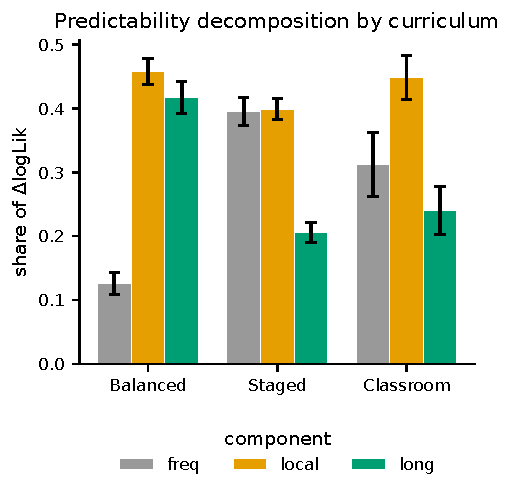
\includegraphics[width=1\linewidth]{fig/interp/D5_decomp_shares.pdf}
    \caption{\textbf{D5 --- Predictability decomposition by curriculum.} Stacked-bar decomposition of the MECO~L2 $\Delta\log L$ share (y-axis) attributable to (i) word log-frequency, (ii) local-context surprisal, and (iii) long-context surprisal, broken out by Beetle curriculum (x-axis: B1--B5; nld--eng). Headline: balanced B1 leans more on word-frequency and local-context predictors than staged B2/B3-33/B5, which redistribute share toward long-context surprisal.}
    \label{fig:D5_decomp_shares}
\end{figure}

\begin{figure}
    \centering
    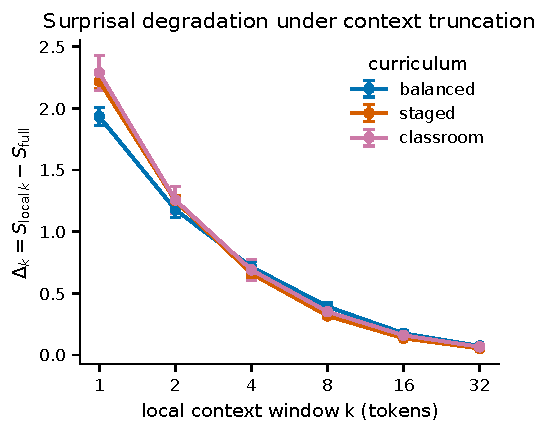
\includegraphics[width=1\linewidth]{fig/interp/D6_context_degradation.pdf}
    \caption{\textbf{D6 --- Surprisal degradation under context truncation.} Per-curriculum surprisal degradation $\Delta_k = S_{\mathrm{local},k} - S_{\mathrm{full}}$ (y-axis) as a function of the local context window size $k$ in tokens (x-axis), for Beetle B1--B5 nld--eng. Larger $\Delta_k$ at small $k$ indicates greater reliance on long-range context. Headline: balanced B1 degrades more than staged B2/B3-33/B5 under aggressive context truncation, consistent with B1 distributing predictive mass across longer contexts.}
    \label{fig:D6_context_degradation}
\end{figure}

\begin{figure}
    \centering
    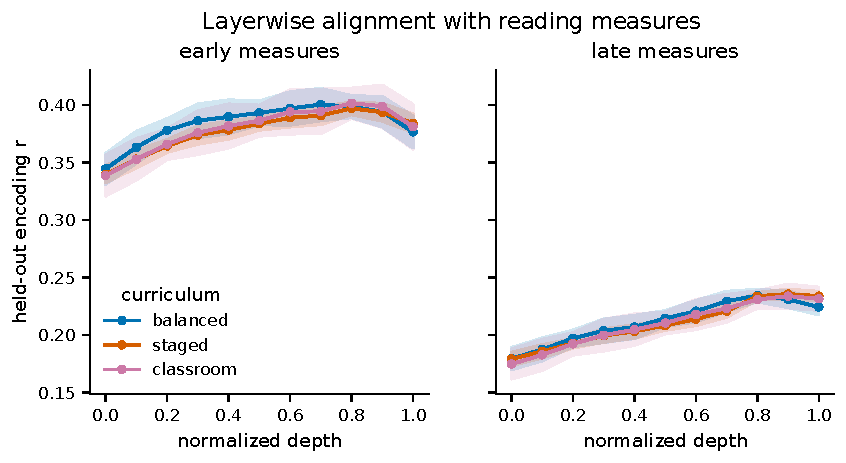
\includegraphics[width=1\linewidth]{fig/interp/D8_layerwise_profile.pdf}
    \caption{\textbf{D8 --- Layerwise alignment with reading measures.} Held-out encoding $r$ between Beetle layer activations and MECO~L2 reading-time measures (y-axis: held-out $r$; x-axis: normalized depth, $0 = $ embedding, $1 = $ final layer). One panel per reading measure (first-pass duration / refixation / regression-in); colours = curriculum (B1 vs.\ B3-33), nld--eng FineWeb-100M checkpoint. Higher $r$ at mid-depth indicates that the corresponding layer linearly explains more reading-time variance.}
    \label{fig:D8_layerwise_profile}
\end{figure}


\begin{figure}
    \centering
    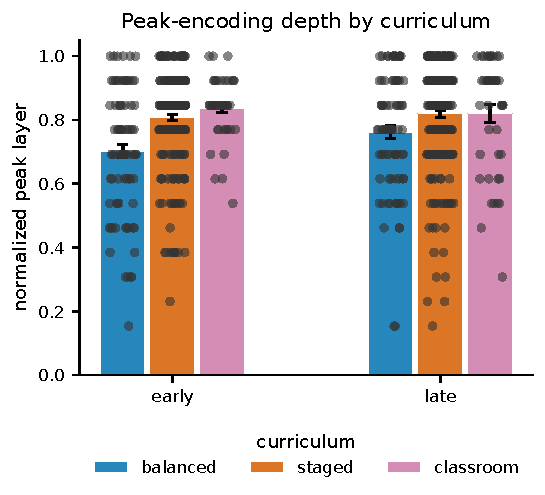
\includegraphics[width=1\linewidth]{fig/interp/D9_peak_layer.pdf}
    \caption{\textbf{D9 --- Peak-encoding depth by curriculum.} Normalized peak layer (y-axis: $0 = $ embedding, $1 = $ final layer) at which the Beetle layer activations most strongly align with each MECO~L2 reading-time measure, broken out by curriculum (x-axis: B1--B5; nld--eng FineWeb-100M). Headline: balanced B1 places its peak-encoding layer deeper in the stack than staged B2/B3-33/B5, consistent with B1 carrying reading-time signal in late integration layers while staged curricula concentrate it in mid-depth layers.}
    \label{fig:D9_peak_layer}
\end{figure}



\begin{figure}
    \centering
    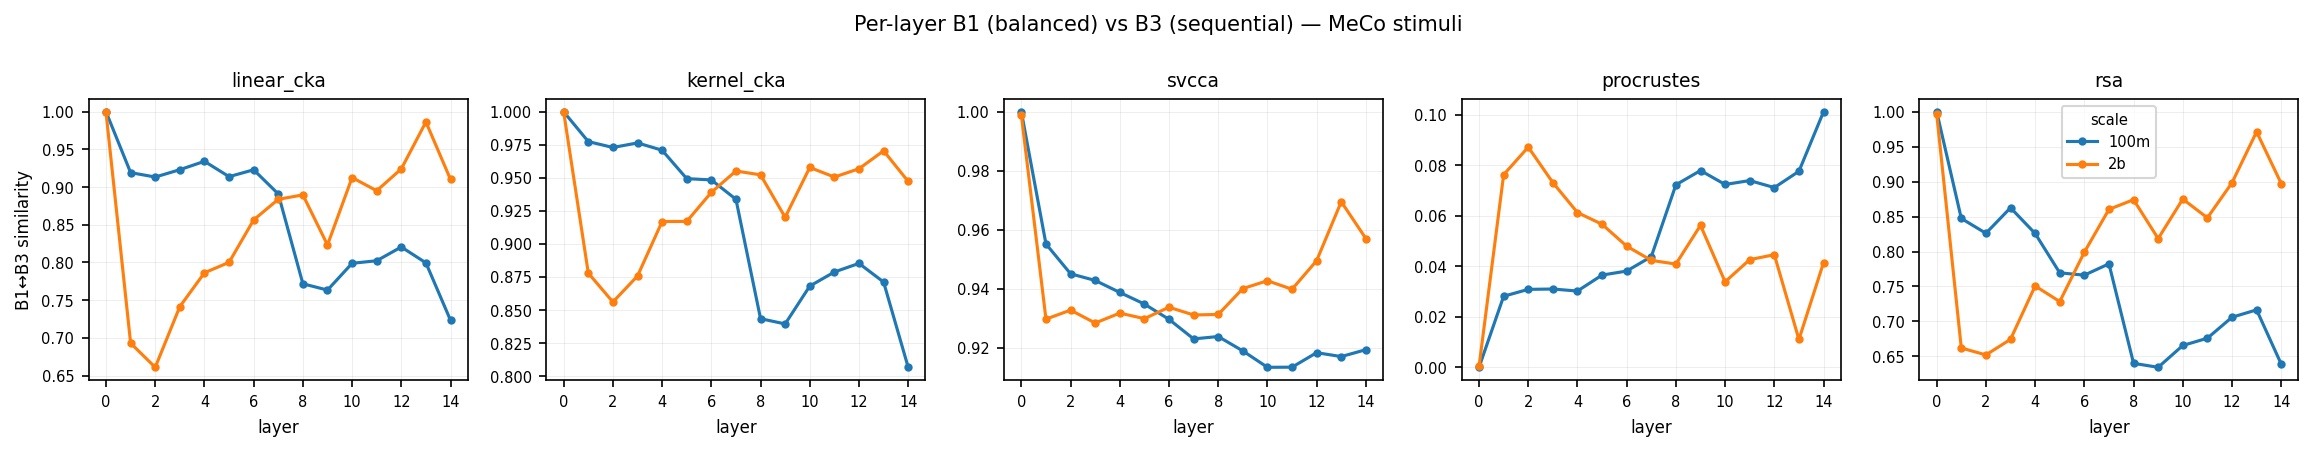
\includegraphics[width=1\linewidth]{fig/interp/repsim_b1_vs_b3.png}
    \caption{\textbf{Representational similarity between B1 balanced and B3-33 sequential, layer-wise.} Four-panel comparison of CKA, RSA, Procrustes, and SVCCA similarity (y-axis, $\in [0,1]$, $\uparrow$ more similar) between B1 balanced and B3-33 sequential nld--eng Beetle activations across layer index (x-axis, embedding $\to$ output). Headline: similarity stays near unity through the embedding and early-block layers but drops sharply at mid-to-late depth, isolating the curriculum-induced representational divergence to the layers most predictive of MECO~L2 reading times (Fig.~\ref{fig:D8_layerwise_profile}).}
    \label{fig:repsim_b1_vs_b3}
\end{figure}

\begin{figure}
    \centering
    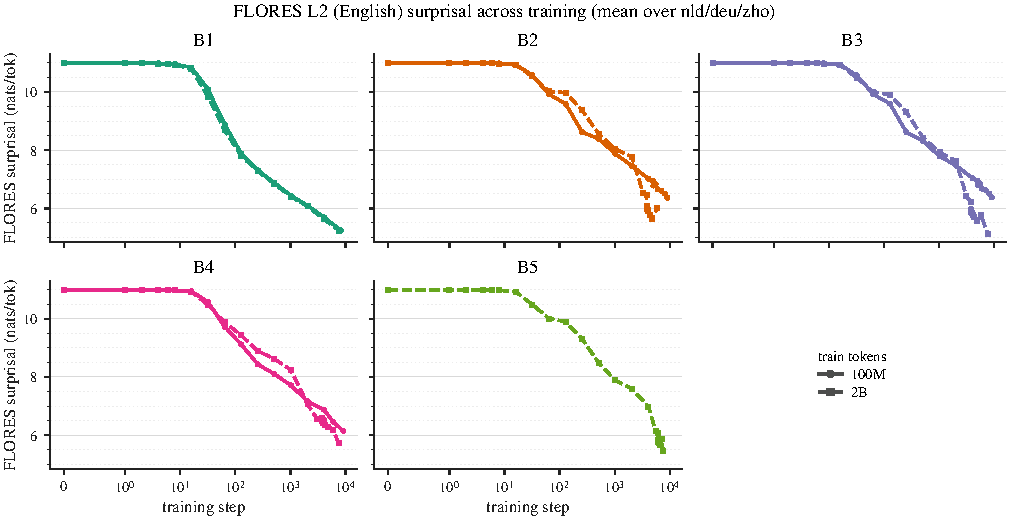
\includegraphics[width=1\linewidth]{fig/flores/fig_flores_main.pdf}
    \caption{\textbf{FLORES~L2 (English) surprisal across training.} Six-panel grid (one panel per curriculum B1--B5; sixth panel is the legend) plotting mean per-token FLORES-200 surprisal (y-axis: nats/tok $=$ log-PPL; $\downarrow$ better) against training step (x-axis: symlog), with 100\,M (solid) and 2\,B (dashed) cohorts overlaid and means taken over nld/deu/zho language pairs. Headline: structured-exposure curricula (B2/B3-33/B5) cross the B-GPT non-forgetting envelope earlier in training than balanced B1 and remain inside it at convergence; no Beetle curriculum exhibits the legacy B-GPT \textsc{nl-en} sequential catastrophic-forgetting failure mode.}
    \label{fig:flores_main}
\end{figure}

\begin{figure}
    \centering
    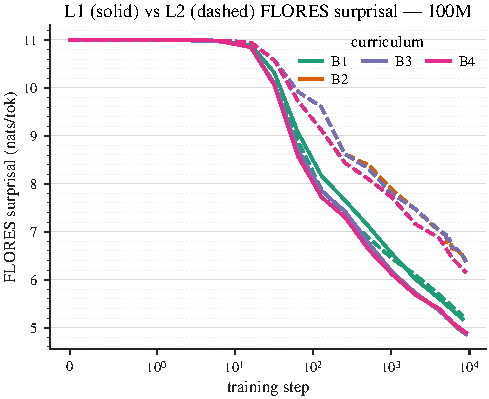
\includegraphics[width=1\linewidth]{fig/flores/fig_flores_l1l2.pdf}
    \caption{\textbf{FLORES~L1 vs.~L2 surprisal, per curriculum.} Single panel showing mean per-token FLORES-200 surprisal (y-axis: nats/tok $=$ log-PPL) across training steps for L1 (solid lines) and L2 English (dashed lines), with colour by Beetle curriculum (B1--B5; matched nld--eng). Headline: late-onset B5 retains tighter L1 surprisal than balanced B1 throughout training; all curricula achieve comparable L2 English asymptotes.}
    \label{fig:flores_l1l2}
\end{figure}


\begin{figure}
    \centering
    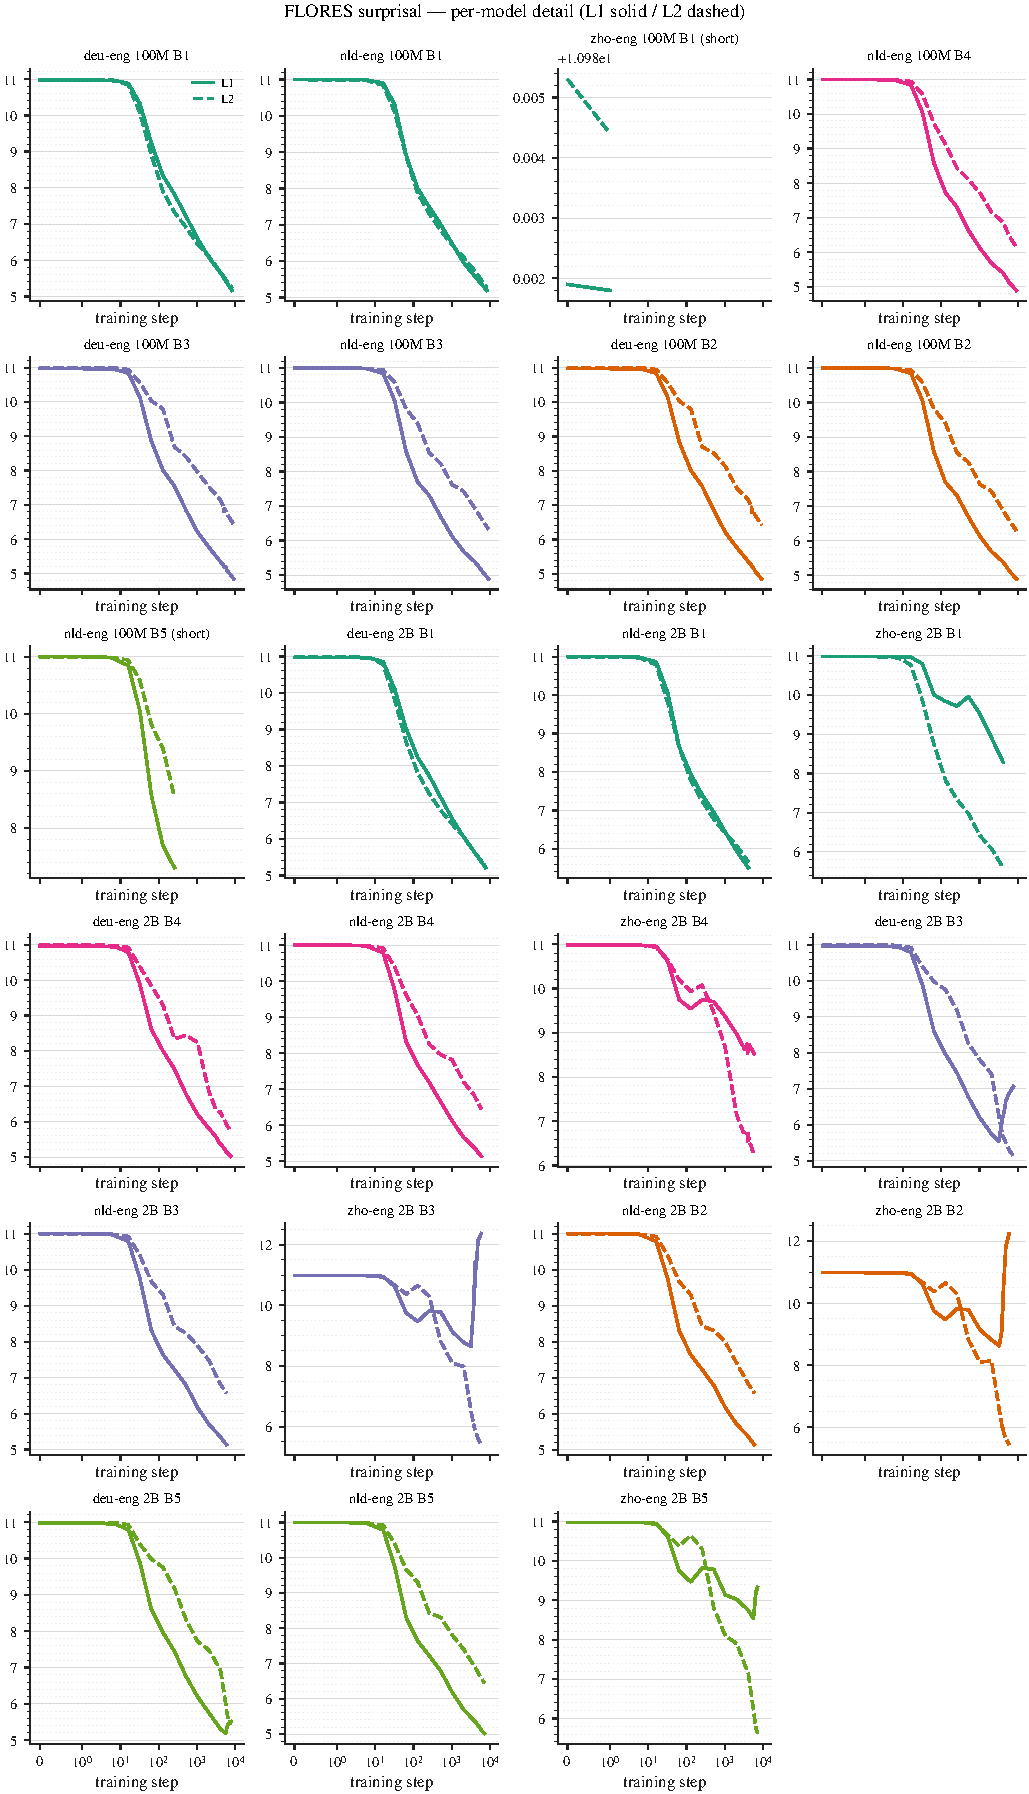
\includegraphics[width=1\linewidth]{fig/flores/appx_flores_per_model.pdf}
    \caption{\textbf{Per-model FLORES-200 surprisal across the full Beetle sweep.} Exhaustive grid plotting mean per-token FLORES-200 surprisal (y-axis: nats/tok $=$ log-PPL) for L1 and L2 English across every Beetle (L1, scale, curriculum) cell. Empty cells indicate runs not yet trained; the zho-100M-B1 cell is shown for completeness but pending a retrain pass.}
    \label{fig:appx_flores_per_model}
\end{figure}


\subsection{Cross-model interpretability diagnostics overview}\label{sec:pico-cross-comp}

The Q1 (L1 + curriculum) and Q2 (correlation) sweeps below jointly constitute the cross-model interpretability diagnostics referenced from the body. Q1 isolates which interpretability metric carries the largest cross-L1 / cross-curriculum signal; Q2 measures how each metric covaries with the downstream evaluation axes (BLiMP, MECO, BLiSS) across the same matched cohort.

\subsection{Q1 --- How does interpretability differ between models?}\label{sec:pico-q1}

\begin{figure}[!ht]
  \centering
  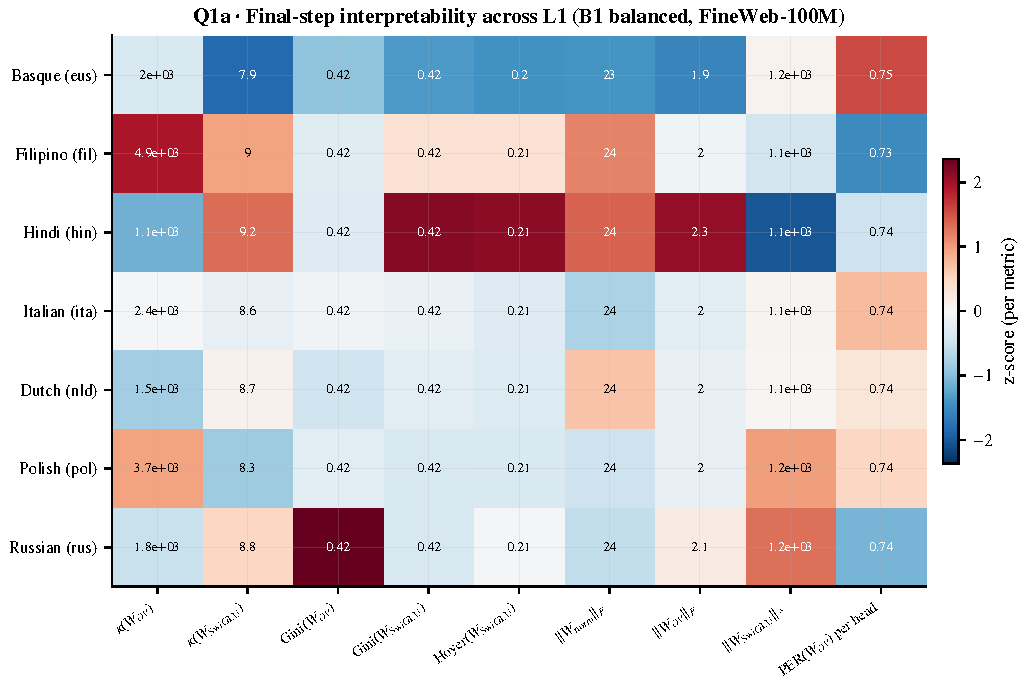
\includegraphics[width=\linewidth]{fig/pico_q1a_l1_heatmap.pdf}
  \caption{\textbf{Q1a -- L1 heatmap.} Final-step layer-mean of every \textsc{Pico-Analyze} interpretability metric against every L1 (B1 only). Cell colour is the per-metric $z$-score; cell text is the raw value. The dominant cross-L1 signal sits in $\kappa(W_{OV})$, which spans an order of magnitude (Dutch $\sim\!1.5\!\times\!10^{3}$ to Hindi $\sim\!1.1\!\times\!10^{4}$). Other metrics are nearly flat across L1 despite the L1s spanning four typological groupings (Germanic, Romance, Slavic, Indo-Aryan, Austronesian, isolate), suggesting that the OV-circuit's spectral conditioning encodes typological distance from the L2 (English) far more sensitively than any sparsity-style metric does.}
  \label{fig:pico-q1a}
\end{figure}

\begin{figure}[!ht]
  \centering
  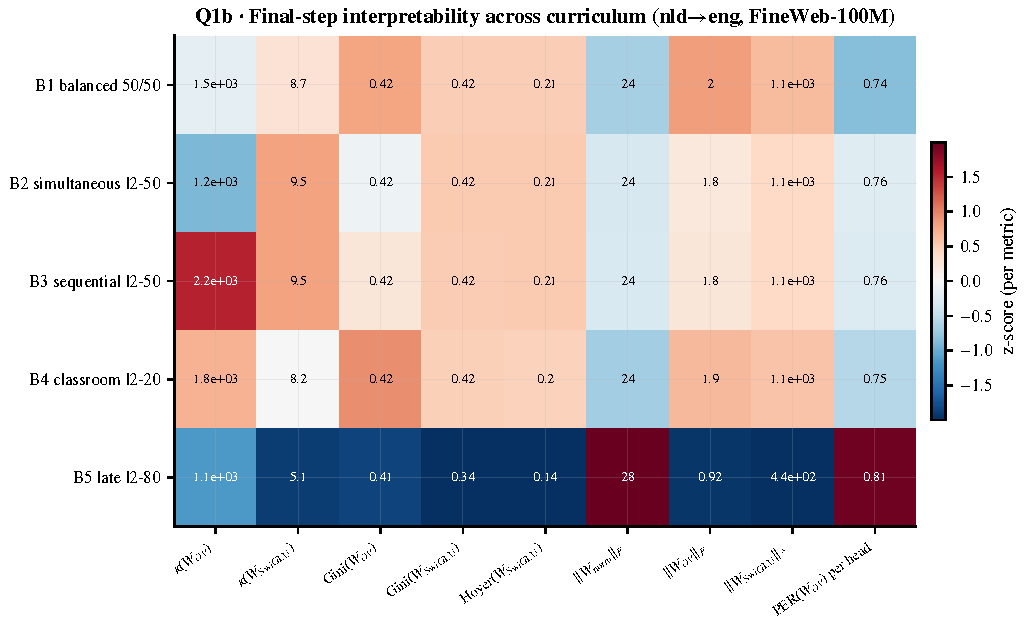
\includegraphics[width=\linewidth]{fig/pico_q1b_curriculum_heatmap.pdf}
  \caption{\textbf{Q1b -- Curriculum heatmap.} Same construction as Fig.~\ref{fig:pico-q1a}, sliced over the nld--eng curriculum sweep (B1--B5). B5 (late l2-80) is the standout outlier on \texttt{gini-swiglu}, \texttt{hoyer-swiglu}, $\Vert W_{OV}\Vert_F$ and $\Vert W_{\text{SwiGLU}}\Vert_*$: its SwiGLU weights are markedly less sparse and the OV norm is depressed (0.92 vs.\ $\sim\!1.78$--$2.02$ for B1--B4). Delaying L2 exposure to 80\% of training prevents the OV circuit from acquiring the high-norm, high-sparsity geometry the other curricula reach.}
  \label{fig:pico-q1b}
\end{figure}

\begin{figure}[!ht]
  \centering
  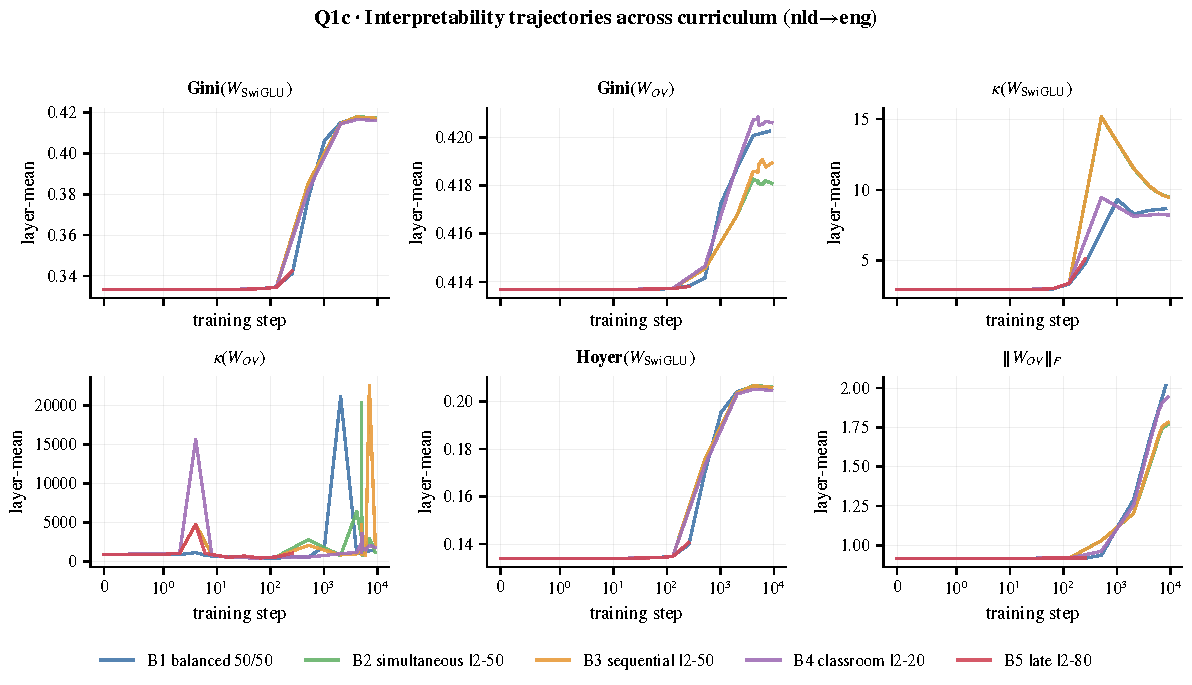
\includegraphics[width=\linewidth]{fig/pico_q1c_curriculum_trajectories.pdf}
  \caption{\textbf{Q1c -- Curriculum trajectories.} Layer-mean trajectories across training step for the B1--B5 nld--eng curricula on six representative interpretability metrics. All metrics emerge between step 256 and 1024 and saturate by 8k; B5 follows the same trajectory shape but at a depressed plateau, indicating that the curriculum effect is one of \emph{plateau height} rather than \emph{onset timing}.}
  \label{fig:pico-q1c}
\end{figure}

\begin{figure}[!ht]
  \centering
  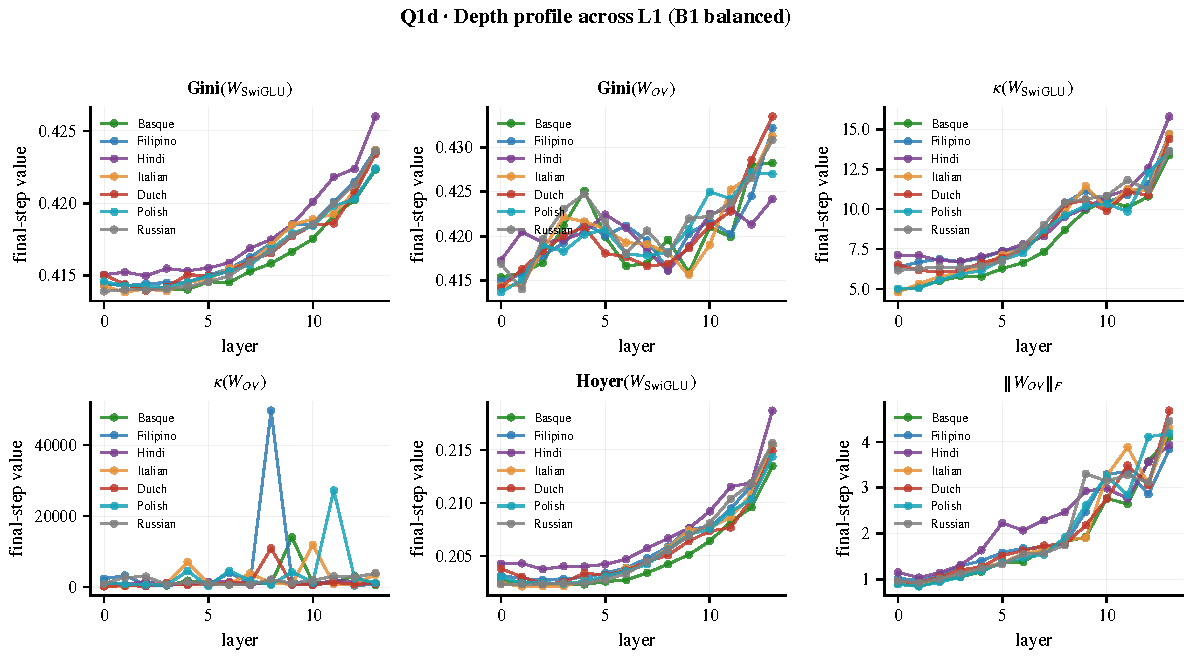
\includegraphics[width=\linewidth]{fig/pico_q1d_depth_profile_l1.pdf}
  \caption{\textbf{Q1d -- Depth profile across L1.} Final-step value as a function of layer index, one panel per metric, lines = L1 (B1 only). The OV-circuit signal is concentrated in mid-to-late layers; sparsity metrics (Gini, Hoyer) are layer-flat. Read together with Fig.~\ref{fig:pico-q1a}, this localises the typological-distance signal to the same depth band that hosts the OV induction circuitry.}
  \label{fig:pico-q1d}
\end{figure}

\begin{figure}[!ht]
  \centering
  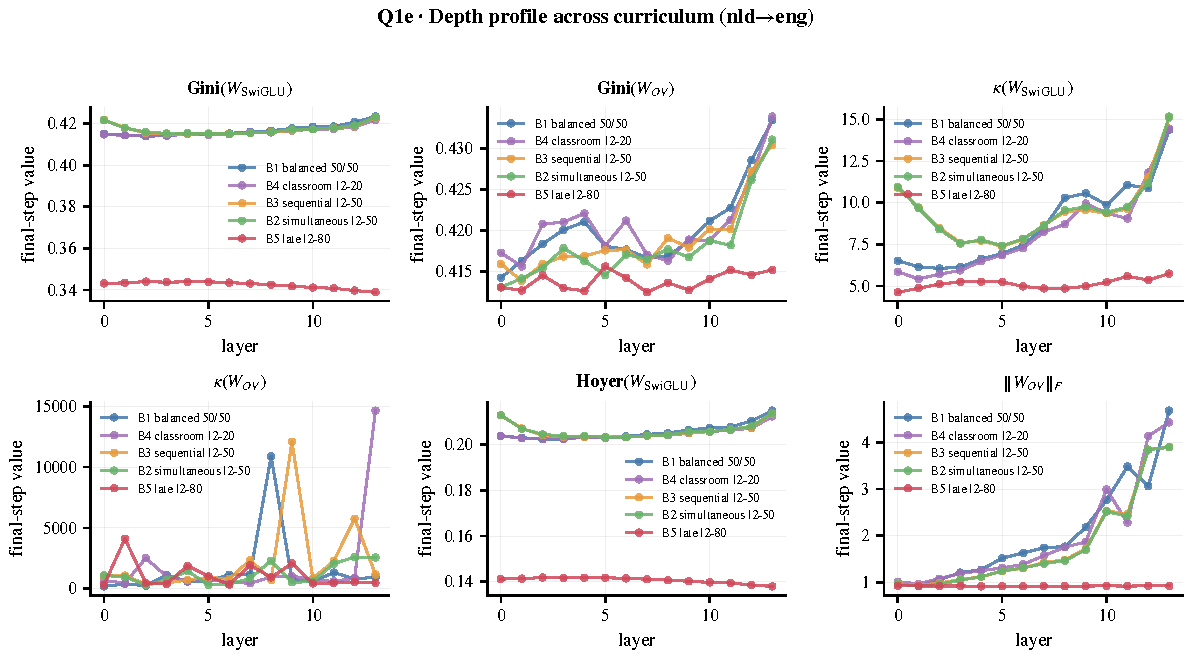
\includegraphics[width=\linewidth]{fig/pico_q1e_depth_profile_curriculum.pdf}
  \caption{\textbf{Q1e -- Depth profile across curriculum.} Same construction as Fig.~\ref{fig:pico-q1d}, lines = curriculum (B1--B5, nld--eng). The B5-vs-B1--B4 plateau gap of Fig.~\ref{fig:pico-q1c} is concentrated in mid-to-late layers, again co-localising with the OV induction band.}
  \label{fig:pico-q1e}
\end{figure}

\subsection{Q2 --- Do interpretability metrics correlate with downstream behaviour?}\label{sec:pico-q2}

\begin{figure}[!ht]
  \centering
  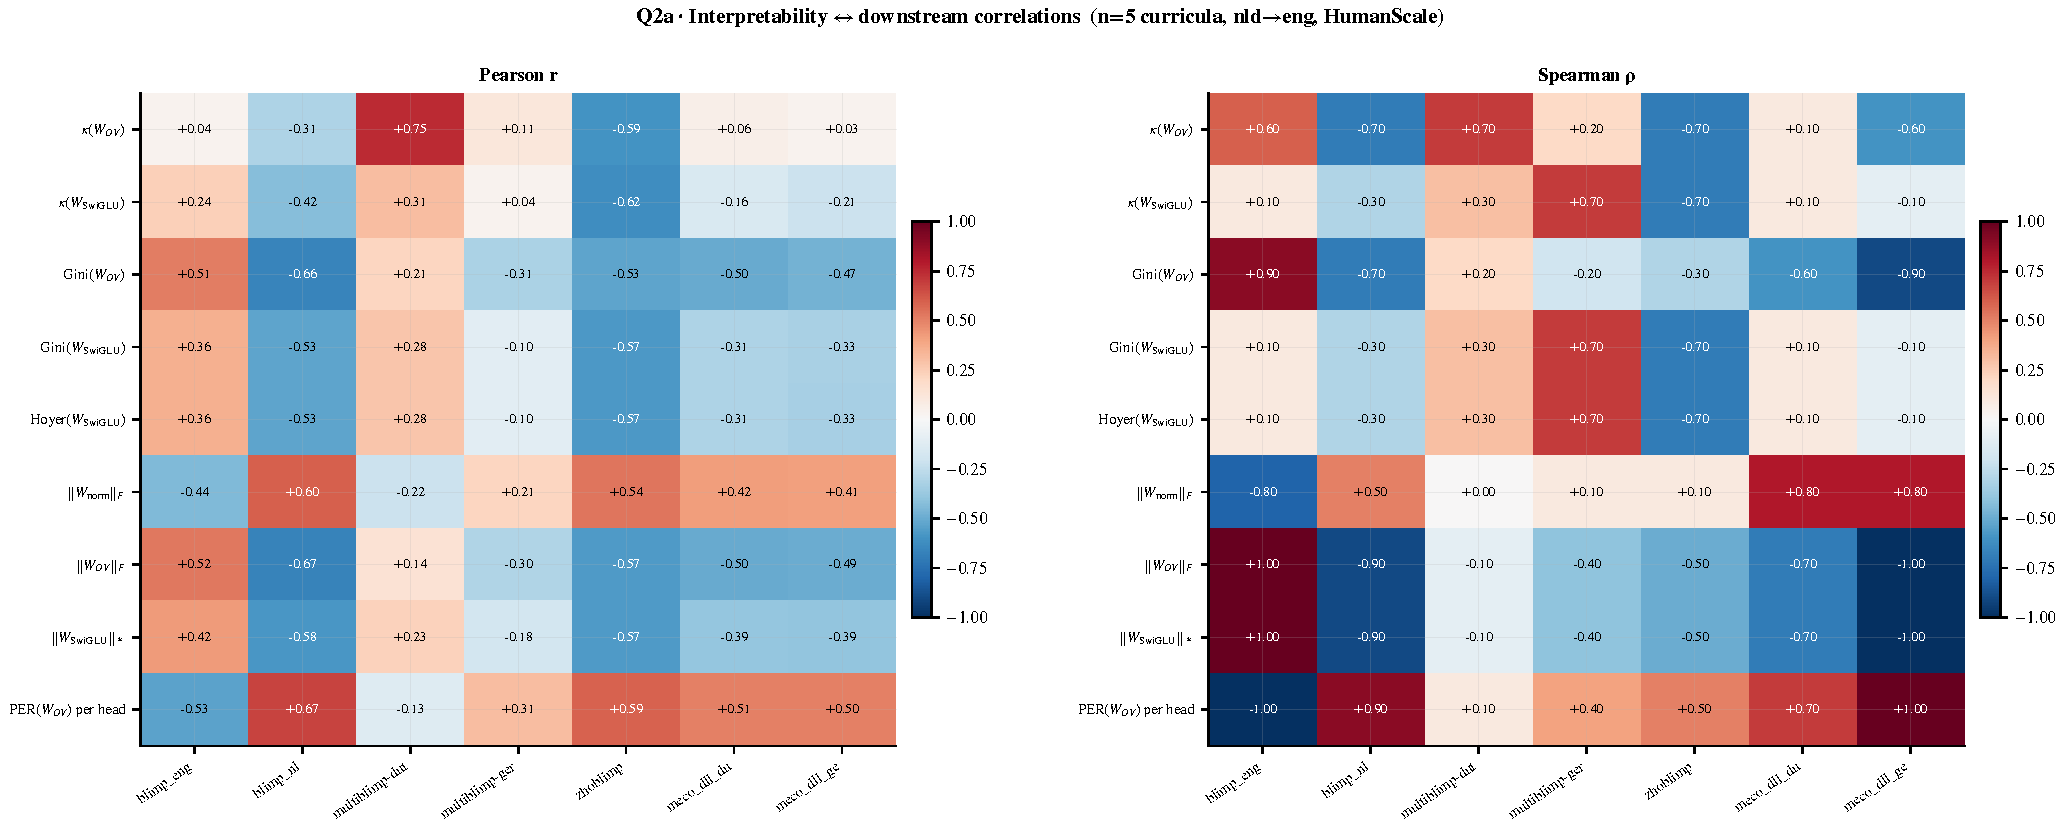
\includegraphics[width=\linewidth]{fig/pico_q2a_corr_heatmap.pdf}
  \caption{\textbf{Q2a -- Correlation heatmap.} Pearson $r$ and Spearman $\rho$ for every (interpretability metric $\times$ downstream metric) pair across the nld--eng curriculum sweep ($n=5$). The signal is asymmetric: sparsity/norm metrics on the OV+SwiGLU subspace track L2 (English) BLiMP performance, but anti-predict the L1-side BLiMP and human-RT alignment. The attention-norm Frobenius $\Vert W_{\text{norm}}\Vert_F$ is the only metric that positively predicts both Dutch BLiMP and MECO surprisal-fit, consistent with B5's larger attention-LayerNorm scales (a more ``spread'' attention pattern). $\kappa(W_{OV})$ is uninformative for the curriculum sweep ($|r|\le 0.31$) yet was the most informative metric across L1s in Q1a --- the same metric carries different signal on different sweep axes.}
  \label{fig:pico-q2a}
\end{figure}

\begin{figure}[!ht]
  \centering
  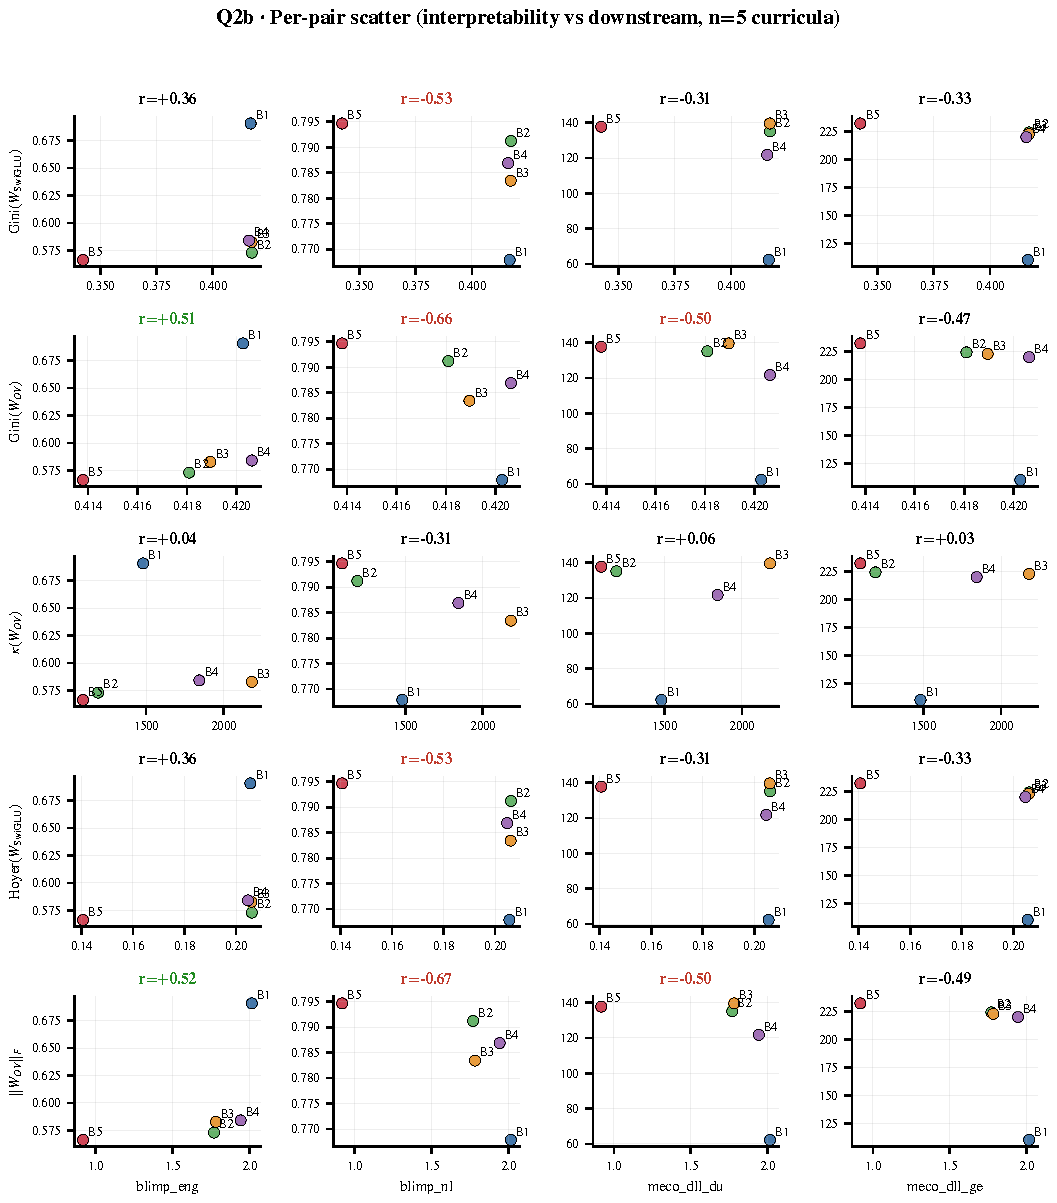
\includegraphics[width=\linewidth]{fig/pico_q2b_scatter_grid.pdf}
  \caption{\textbf{Q2b -- Per-pair scatter.} Scatter for a curated subset of (interpretability metric $\times$ downstream metric) pairs over the $n=5$ nld--eng curricula. Curriculum labels (B1--B5) annotated on each panel; per-panel Pearson $r$ in the title. The B1$\leftrightarrow$B5 separation along $\Vert W_{OV}\Vert_F$ and Gini$(W_{\text{SwiGLU}})$ is visible directly in the per-panel point cloud; treat the regression slopes as exploratory at $n=5$.}
  \label{fig:pico-q2b}
\end{figure}

\begin{figure}[!ht]
  \centering
  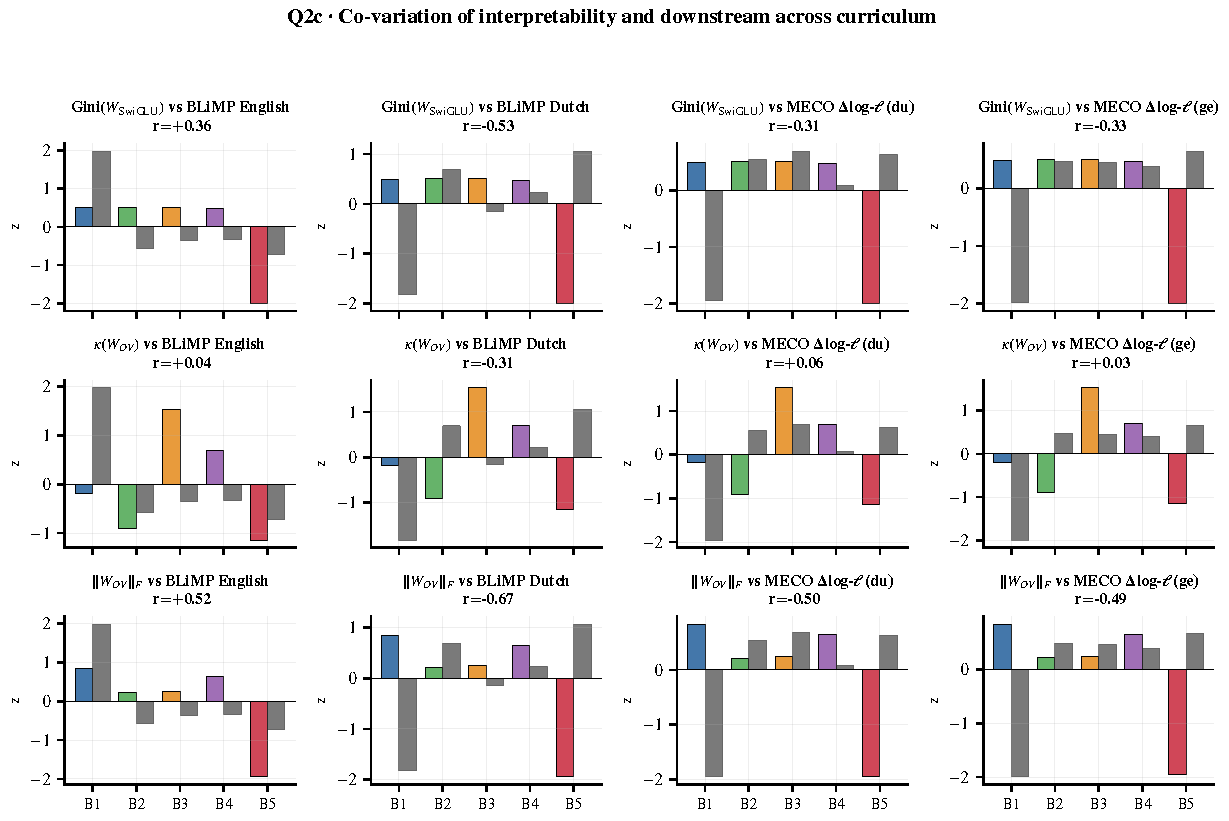
\includegraphics[width=\linewidth]{fig/pico_q2c_paired_bars.pdf}
  \caption{\textbf{Q2c -- Paired $z$-scored bars.} For each curriculum (B1--B5), each interpretability metric is paired with a downstream metric on a common $z$-axis. Co-variation is read as ``same height $\Rightarrow$ same direction''; sign-flip clusters --- e.g.\ $\Vert W_{OV}\Vert_F$ vs.\ BLiMP-nl, Gini$(W_{\text{SwiGLU}})$ vs.\ MECO~du --- visualise the specialisation--generalisation trade-off referenced in \S\ref{sec:pico-cross-comp}.}
  \label{fig:pico-q2c}
\end{figure}

\subsection{Principal correlations and summary}\label{sec:pico-headline}

The principal Q2 results, exact reproductions of the per-pair Pearson $r$ values plotted in Fig.~\ref{fig:pico-q2a} and tabulated in \texttt{ledger\_q2\_joined.csv}, are summarised in Table~\ref{tab:pico-q2-headline}.

\begin{table}[h]
  \centering
  \small
  \caption{Pearson $r$ across the $n=5$ nld--eng curriculum sweep (B1--B5) for selected (interpretability metric, downstream metric) pairs. Bold cells exceed $|r|>0.5$. From \texttt{ledger\_q2\_joined.csv}.}
  \label{tab:pico-q2-headline}
  \begin{tabular}{lrrrr}
    \toprule
    metric & BLiMP-eng & BLiMP-nl & MECO-du & MECO-ge \\
    \midrule
    $\Vert W_{OV}\Vert_F$       & \textbf{+0.52} & \textbf{$-$0.67} & $-$0.50 & $-$0.49 \\
    Gini$(W_{\text{SwiGLU}})$   & $+$0.36        & \textbf{$-$0.53} & $-$0.31 & $-$0.33 \\
    Hoyer$(W_{\text{SwiGLU}})$  & $+$0.36        & \textbf{$-$0.53} & $-$0.37 & $-$0.33 \\
    $\Vert W_{\text{norm}}\Vert_F$ & $-$0.44     & \textbf{$+$0.60} & \textbf{$+$0.54} & $+$0.42 \\
    $\kappa(W_{OV})$            & $+$0.04        & $-$0.31          & $+$0.06 & $+$0.03 \\
    \bottomrule
  \end{tabular}
\end{table}

\paragraph{Take-home.} The interpretability metrics in \textsc{Pico-Analyze} do not measure a single latent ``model quality'' axis. They measure \emph{specialisation vs.\ generalisation}: high Gini/Hoyer/Frobenius on the OV+SwiGLU subspaces buy English BLiMP at the cost of L1 transfer and psycholinguistic alignment. The curriculum that maximises BLiMP-eng (B1, balanced 50/50) and the curriculum that maximises L1 retention and human-RT alignment (B5, late l2-80) lie at opposite ends of the same axis the interpretability metrics are sensitive to.

\paragraph{Caveats.} (i) $n=5$ for every Q2 correlation; treat $r$-values as exploratory; bootstrap CIs over the curriculum sweep are pending. (ii) Downstream evaluations are at \textsc{HumanScale} (0.1~B token); interpretability metrics are at \textsc{FineWeb}-100M ($\sim$0.1~B token). Same parameter count and effective token budget, but the corpora differ; a matched-corpus re-run (interpretability on \textsc{HumanScale} checkpoints) would tighten the join. (iii) \textsc{BLiSS} excluded as noted above. (iv) \textsc{Pico} run \texttt{beetle-bilingual-balanced-b1-fineweb-100m-rus-eng} contributes to Q1 only.

\section{Detailed Downstream Results}\label{sec:downstream}

This section consolidates the body sanity-check tables (\textsc{MultiBLiMP}, \textsc{FLORES-200} PPL, catastrophic-forgetting) at full resolution. \textsc{MultiBLiMP} per-language accuracy (Tab.~\ref{tab:multiblimp}) confirms that B3-33 nld--eng reaches 90.3\% Dutch grammaticality (best \textsc{Beetle} cell), and that the structured-exposure advantage attenuates monotonically across the typological distance gradient (Dutch~$>$~German~$>$~French~$>$~Persian~$>$~Bulgarian). \textsc{FLORES-200} per-language PPL and $\Delta$-NLL relative to the matched monolingual anchor (Tab.~\ref{tab:flores_ppl}) confirm that B1 balanced and B2 simultaneous incur the smallest L1 PPL penalty after L2 introduction; the catastrophic-forgetting aggregation by acquisition schedule (Tab.~\ref{tab:forgetting}) closes the per-curriculum sanity ledger. \label{appcomp:phase}

\begin{table}[t]
  \centering
  \small
  \caption{\textsc{MultiBLiMP} accuracy (\%) across five languages for nld-eng \textsc{HumanScale} \beetle{} models and baselines. Bold marks the best per-column result.}
  \label{tab:multiblimp}
  \begin{tabular}{lrrrrr}
    \toprule
    Condition & Dutch & German & French & Persian & Bulgarian \\
    \midrule
    mono-ENG & 53.0 & 60.3 & 60.8 & 52.9 & 63.5 \\
    mono-NLD & 88.9 & 67.4 & 58.9 & 40.4 & 62.4 \\
    B1       & 87.6 & 67.6 & 61.5 & 53.4 & 62.5 \\
    B2       & 88.8 & 73.3 & 63.3 & 49.5 & 62.4 \\
    B3-33    & \textbf{90.3} & 72.9 & 62.0 & 51.4 & 62.3 \\
    B3-0     & 89.7 & 70.9 & 61.8 & 51.3 & 62.6 \\
    B4       & 89.8 & 72.3 & 61.5 & 51.6 & 62.3 \\
    B5       & 88.5 & 72.1 & 62.2 & 51.2 & 62.0 \\
    episodic & 86.4 & 70.7 & 61.7 & 54.7 & 61.2 \\
    ewc      & 88.8 & 73.3 & 63.3 & 49.5 & 62.4 \\
    lamol    & 88.8 & 73.3 & 63.3 & 49.5 & 62.4 \\
    BLOOM-560m & 59.1 & 65.8 & 81.4 & 55.5 & 58.8 \\
    BLOOM-1b1  & 62.8 & 76.5 & 94.0 & 55.6 & 64.3 \\
    BLOOM-1b7  & 65.9 & 75.8 & 93.1 & 57.9 & 64.7 \\
    BLOOM-3b   & 65.6 & 80.6 & \textbf{97.9} & 59.9 & 63.9 \\
    BLOOM-7b1  & 64.6 & \textbf{82.7} & 95.3 & \textbf{60.1} & \textbf{67.2} \\
    \bottomrule
  \end{tabular}
\end{table}

\begin{table}[t]
  \centering
  \tiny
  \caption{\textsc{FLORES-200} per-sentence perplexity (PPL, lower is better) and $\Delta$-NLL relative to the best monolingual baseline per language (negative = lower PPL than monolingual). Bold marks minimum PPL / $\Delta$-NLL closest to zero per language.}
  \label{tab:flores_ppl}
  \begin{tabular}{lrrrrrrrr}
    \toprule
    & \multicolumn{2}{c}{NLD} & \multicolumn{2}{c}{ENG} & \multicolumn{2}{c}{DEU} & \multicolumn{2}{c}{ZHO} \\
    \cmidrule(lr){2-3} \cmidrule(lr){4-5} \cmidrule(lr){6-7} \cmidrule(lr){8-9}
    Condition & PPL & $\Delta$-NLL & PPL & $\Delta$-NLL & PPL & $\Delta$-NLL & PPL & $\Delta$-NLL \\
    \midrule
    mono-ENG       & ---  & ---     & 781  & \textbf{+0.00} & ---  & ---     & ---  & ---     \\
    mono-NLD       & 324  & \textbf{+0.00} & ---  & ---     & ---  & ---     & ---  & ---     \\
    mono-DEU       & ---  & ---     & ---  & ---     & 400  & \textbf{+0.00} & ---  & ---     \\
    mono-ZHO       & ---  & ---     & ---  & ---     & ---  & ---     & \textbf{3839} & \textbf{+0.00} \\
    B1 nld-eng HS  & 318  & +0.02   & 412  & $-$0.57 & ---  & ---     & ---  & ---     \\
    B1 eng-deu FW  & ---  & ---     & 104  & $-$1.87 & \textbf{81}   & $-$1.44 & ---  & ---     \\
    B1 nld-eng FW  & 81   & $-$1.28 & 109  & $-$1.84 & ---  & ---     & ---  & ---     \\
    B2 nld-eng FW  & \textbf{75} & $-$1.40 & 303  & $-$0.87 & ---  & ---     & ---  & ---     \\
    B2 eng-nld FW  & 273  & $-$0.08 & \textbf{94}   & $-$2.01 & ---  & ---     & ---  & ---     \\
    B3-33 nld-eng HS & 268 & $-$0.22 & 1033 & +0.24   & ---  & ---     & ---  & ---     \\
    B3-33 zho-eng HS & --- & ---    & 1277 & +0.50   & ---  & ---     & 7223 & +0.36   \\
    B5 nld-eng HS  & 268  & $-$0.23 & 987  & +0.22   & ---  & ---     & ---  & ---     \\
    BLOOM-1b1      & 402  & +0.23   & 122  & $-$1.78 & ---  & ---     & ---  & ---     \\
    BLOOM-560m     & 7888 & +2.43   & 7625 & +0.33   & ---  & ---     & ---  & ---     \\
    \bottomrule
  \end{tabular}
\end{table}

\begin{table}[t]
  \centering
  \small
  \caption{Catastrophic forgetting aggregated by acquisition schedule and L1, sorted by \% sentences worse ascending. Mean $\Delta$-PPL: mean increase in per-sentence PPL over the matched monolingual baseline. CF Log-Ratio: mean log perplexity ratio (positive = worse). $N$ = number of (model, L2-language) cells contributing. No \beetle{} curriculum exhibits the legacy B-GPT \textsc{nl-en} sequential catastrophic-forgetting failure mode.}
  \label{tab:forgetting}
  \begin{tabular}{llrrrr}
    \toprule
    L1 & Schedule & Mean $\Delta$-PPL & CF Log-Ratio & \% Worse & $N$ \\
    \midrule
    German  & Balanced     & \textbf{157} & \textbf{+0.14} & \textbf{57} & 2 \\
    German  & Sequential   & 286   & +0.34 & 59  & 2 \\
    German  & Part-time    & 396   & +0.48 & 66  & 3 \\
    German  & Heritage     & 2418  & +0.76 & 67  & 6 \\
    German  & Simultaneous & 1111  & +0.61 & 68  & 4 \\
    German  & Late L2      & 118823 & +3.14 & 93 & 4 \\
    Chinese & Simultaneous & 676   & +2.90 & 100 & 1 \\
    Dutch   & Heritage     & 371   & +2.48 & 100 & 2 \\
    Dutch   & Simultaneous & 774   & +3.17 & 100 & 3 \\
    Dutch   & Balanced     & 1048  & +3.24 & 100 & 8 \\
    Chinese & Late L2      & 1445  & +3.63 & 100 & 5 \\
    Chinese & Heritage     & 1498  & +3.63 & 100 & 4 \\
    Chinese & Balanced     & 7350  & +4.42 & 100 & 9 \\
    Dutch   & Late L2      & 35979 & +4.86 & 100 & 2 \\
    Dutch   & Part-time    & 36071 & +5.14 & 100 & 2 \\
    Chinese & Part-time    & 30567 & +6.65 & 100 & 1 \\
    Dutch   & Sequential   & 71758 & +7.66 & 100 & 1 \\
    \bottomrule
  \end{tabular}
\end{table}

\subsection{F-figure reproductions (full resolution)}


\begin{figure}[p]
  \centering
  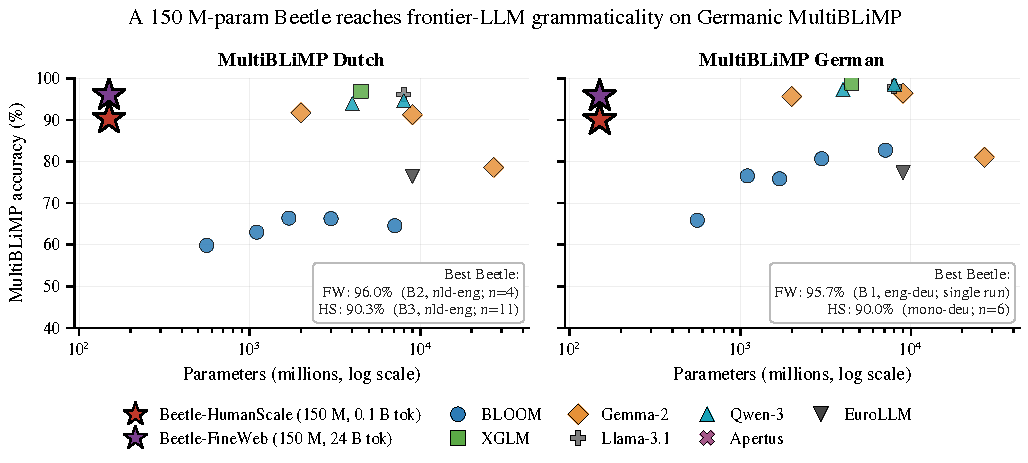
\includegraphics[width=0.86\linewidth,height=0.78\textheight,keepaspectratio]{fig/F1_multiblimp_pareto_baselines.pdf}
  \caption{MultiBLiMP cross-class scatter: per-language grammaticality accuracy for \textsc{Beetle} bilingual curricula B1--B5 (\textsc{HumanScale}~100M and \textsc{FineWeb}~2B token budgets) against the BLOOM 560M--7B1 ladder, XGLM-4.5B, EuroLLM-9B, Apertus-8B, Gemma-2-9B, and Qwen-3 baselines. Companion to the body MultiBLiMP table (Tab.~\ref{tab:multiblimp_efficiency}).}
  \label{appcomp:F1_multiblimp_pareto_baselines}
\end{figure}

\clearpage


\begin{figure}[p]
  \centering
  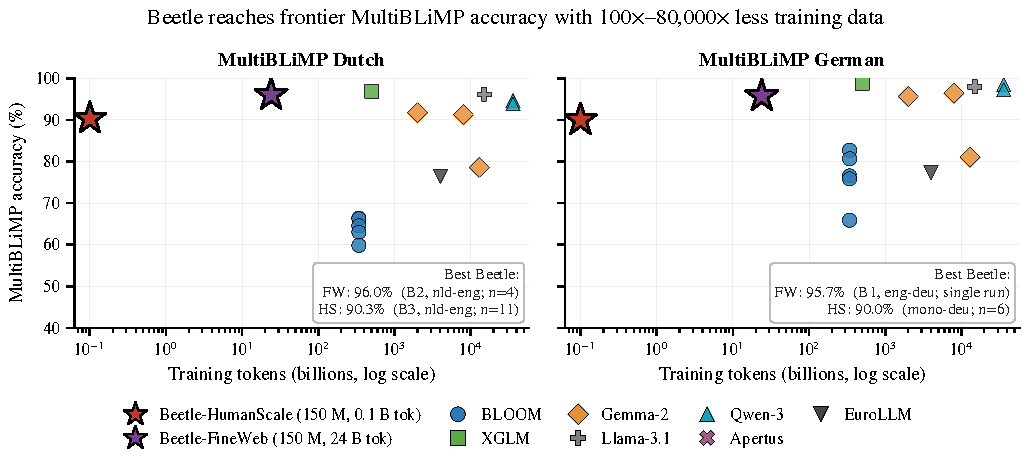
\includegraphics[width=0.86\linewidth,height=0.78\textheight,keepaspectratio]{fig/F2_multiblimp_token_efficiency.pdf}
  \caption{MultiBLiMP Dutch grammaticality accuracy as a function of training tokens (log scale) for \textsc{Beetle} curricula B1--B5 nld--eng compared to the BLOOM ladder and XGLM-4.5B. Companion to main-body Tab.~\ref{tab:multiblimp_efficiency}.}
  \label{appcomp:F2_multiblimp_token_efficiency}
\end{figure}

\begin{figure}[p]
  \centering
  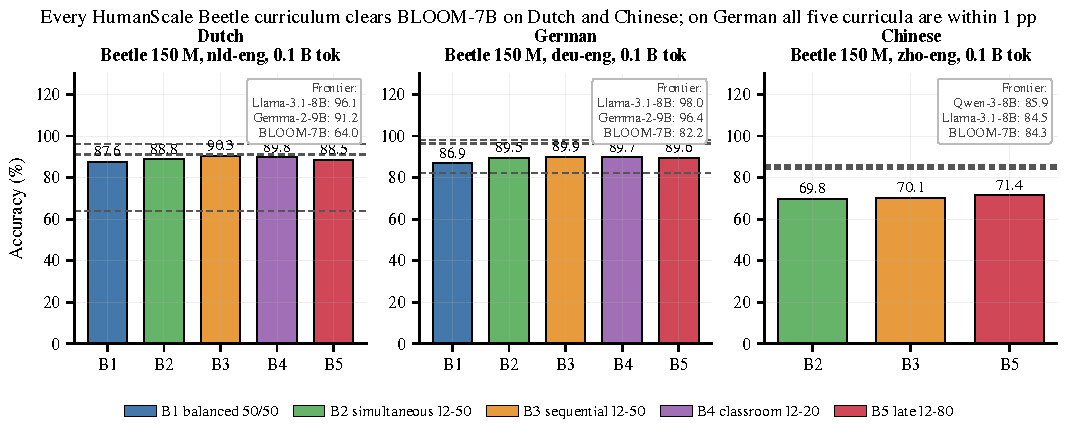
\includegraphics[width=0.86\linewidth,height=0.78\textheight,keepaspectratio]{fig/F3_curriculum_multiblimp.pdf}
  \caption{MultiBLiMP grammaticality accuracy by curriculum (B1--B5) across five target languages (Dutch, German, French, Persian, Bulgarian) for \textsc{Beetle} bilingual nld--eng models at the \textsc{FineWeb}~2B token budget. Reproduced from main-body Fig.~\ref{fig:multiblimp_curriculum}.}
  \label{appcomp:F3_curriculum_multiblimp}
\end{figure}

\begin{figure}[p]
  \centering
  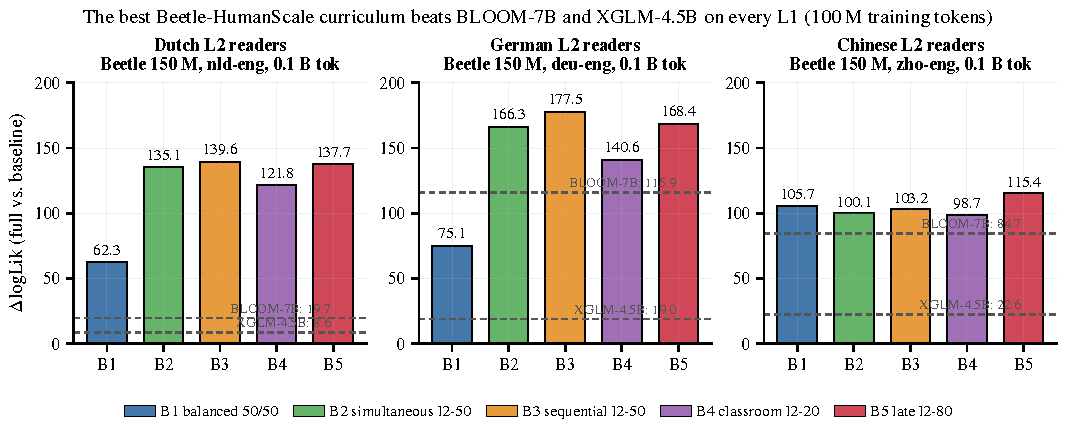
\includegraphics[width=0.86\linewidth,height=0.78\textheight,keepaspectratio]{fig/meco/F4_curriculum_meco_deltaLL.pdf}
  \caption{MECO~L2 $\Delta\log L$ by exposure curriculum (B1--B5) for Dutch, German, and Chinese L2 reader groups, evaluated on the matched MECO~L2 split. The cross-curriculum ordering is the inverse of the MultiBLiMP ordering shown in Fig.~\ref{appcomp:F3_curriculum_multiblimp}; reproduced from main-body Fig.~\ref{fig:meco_curriculum}.}
  \label{appcomp:F4_curriculum_meco_deltaLL}
\end{figure}

\begin{figure}[p]
  \centering
  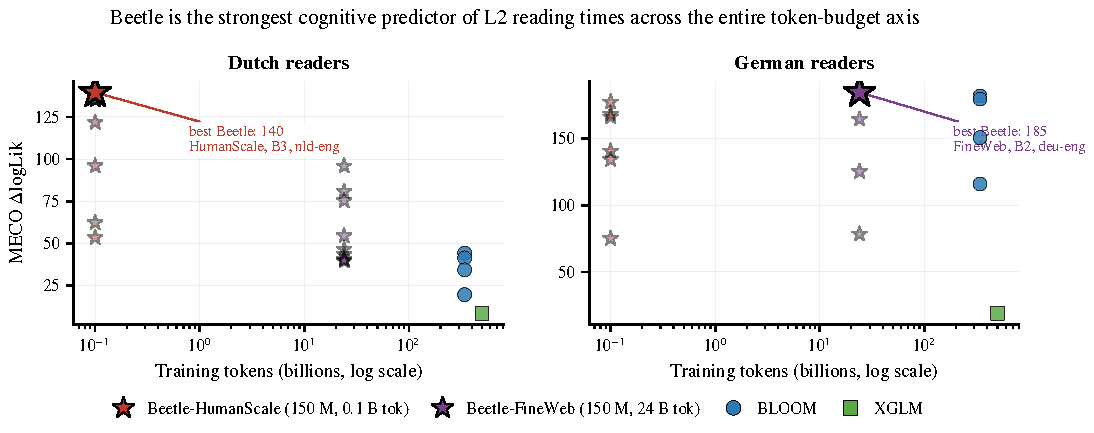
\includegraphics[width=0.86\linewidth,height=0.78\textheight,keepaspectratio]{fig/F5_meco_token_efficiency.pdf}
  \caption{MECO~L2 $\Delta\log L$ as a function of training tokens (log scale) for \textsc{Beetle} curricula B1--B5 (nld--eng and deu--eng) against the BLOOM ladder and XGLM-4.5B. Reproduced from main-body Fig.~\ref{fig:meco_efficiency}.}
  \label{appcomp:F5_meco_token_efficiency}
\end{figure}

\begin{figure}[p]
  \centering
  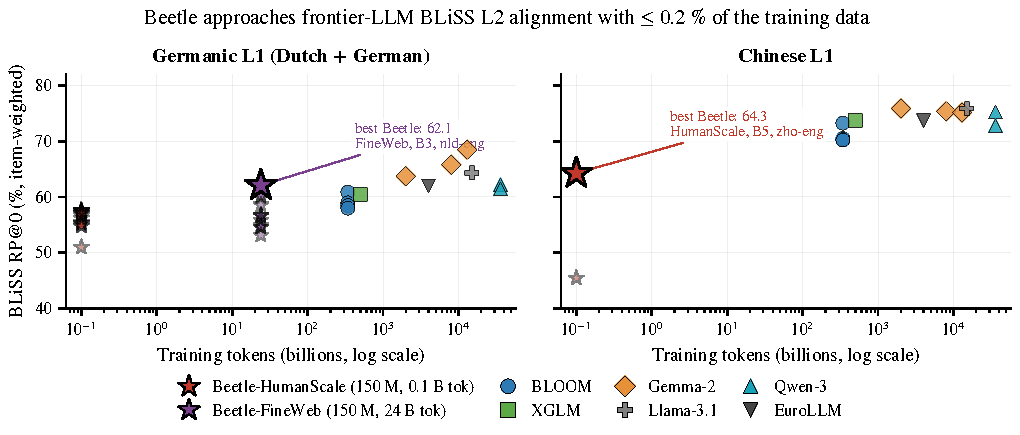
\includegraphics[width=0.86\linewidth,height=0.78\textheight,keepaspectratio]{fig/F6_bliss_token_efficiency.pdf}
  \caption{BLiSS NGS as a function of training tokens for \textsc{Beetle} curricula B1--B5 against the same baselines. Companion to Fig.~\ref{appcomp:F5_meco_token_efficiency}; the curriculum ordering is the inverse of the MECO~L2 ordering.}
  \label{appcomp:F6_bliss_token_efficiency}
\end{figure}


\clearpage


\begin{figure}[!ht]
  \centering
  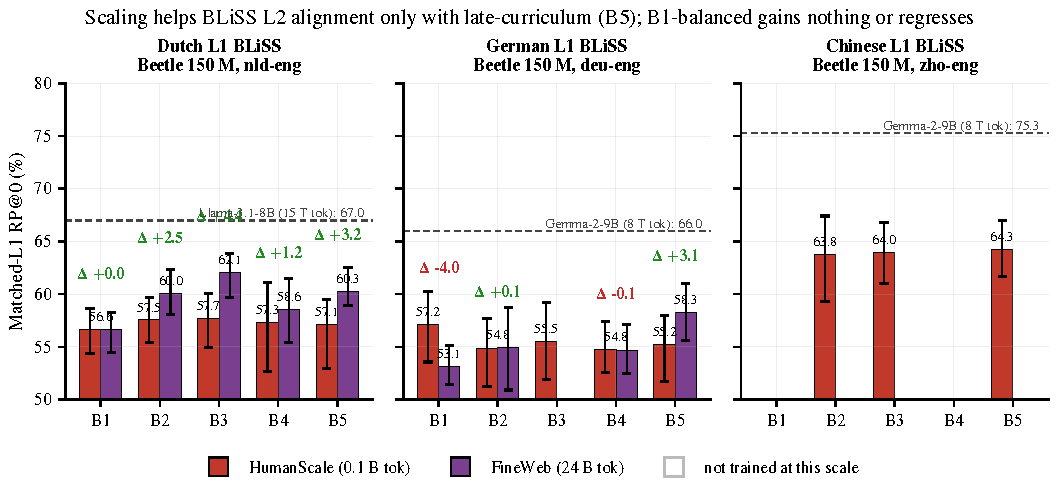
\includegraphics[width=0.86\linewidth,height=0.78\textheight,keepaspectratio]{fig/F7_bliss_curriculum_x_scale.pdf}
  \caption{BLiSS NGS by exposure curriculum $\times$ training scale (\textsc{HumanScale}~100M and \textsc{FineWeb}~2B). Reproduced from main-body Fig.~\ref{fig:bliss_curriculum_scale}.}
  \label{appcomp:F7_bliss_curriculum_x_scale}
\end{figure}

\begin{figure}[p]
  \centering
  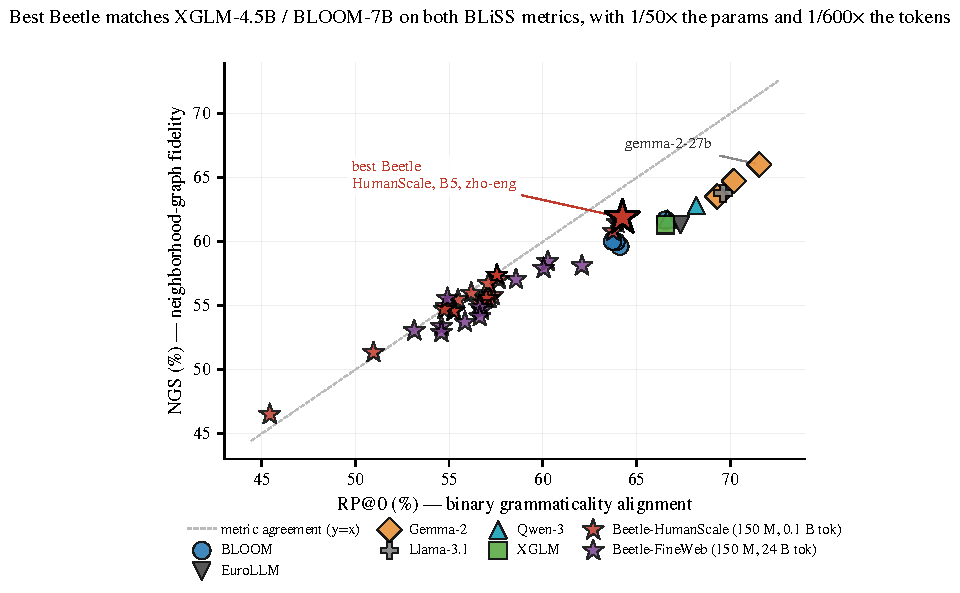
\includegraphics[width=0.86\linewidth,height=0.78\textheight,keepaspectratio]{fig/F8_bliss_metric_tradeoff_pareto.pdf}
  \caption{BLiSS metric trade-off (NGS, CPS, RP$@\tau$) across \textsc{Beetle} curricula and the baseline cohort. Reproduced from main-body Fig.~\ref{fig:bliss_pareto}.}
  \label{appcomp:F8_bliss_metric_tradeoff_pareto}
\end{figure}

\begin{figure*}[!htbp]
  \centering
  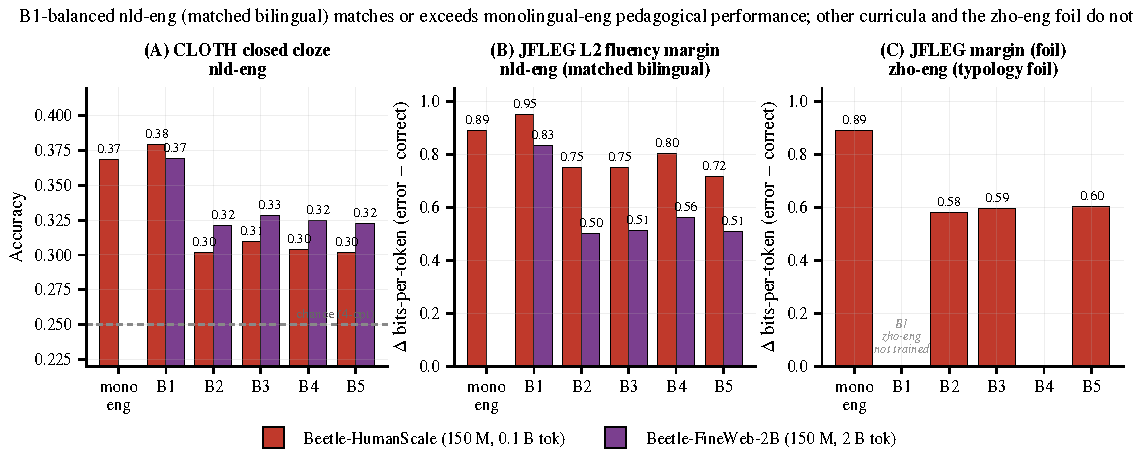
\includegraphics[width=0.86\linewidth,height=0.78\textheight,keepaspectratio]{fig/F9_pedagogical_headline.pdf}
  \caption{Pedagogical evaluation: CLOTH closed-cloze accuracy and JFLEG L2-fluency margin (matched nld--eng; zho--eng foil) by curriculum and training scale. Companion to body Tab.~\ref{tab:headline_pedagogical}.}
  \label{appcomp:F9_pedagogical_headline}
\end{figure*}

\begin{figure*}[!htbp]
  \centering
  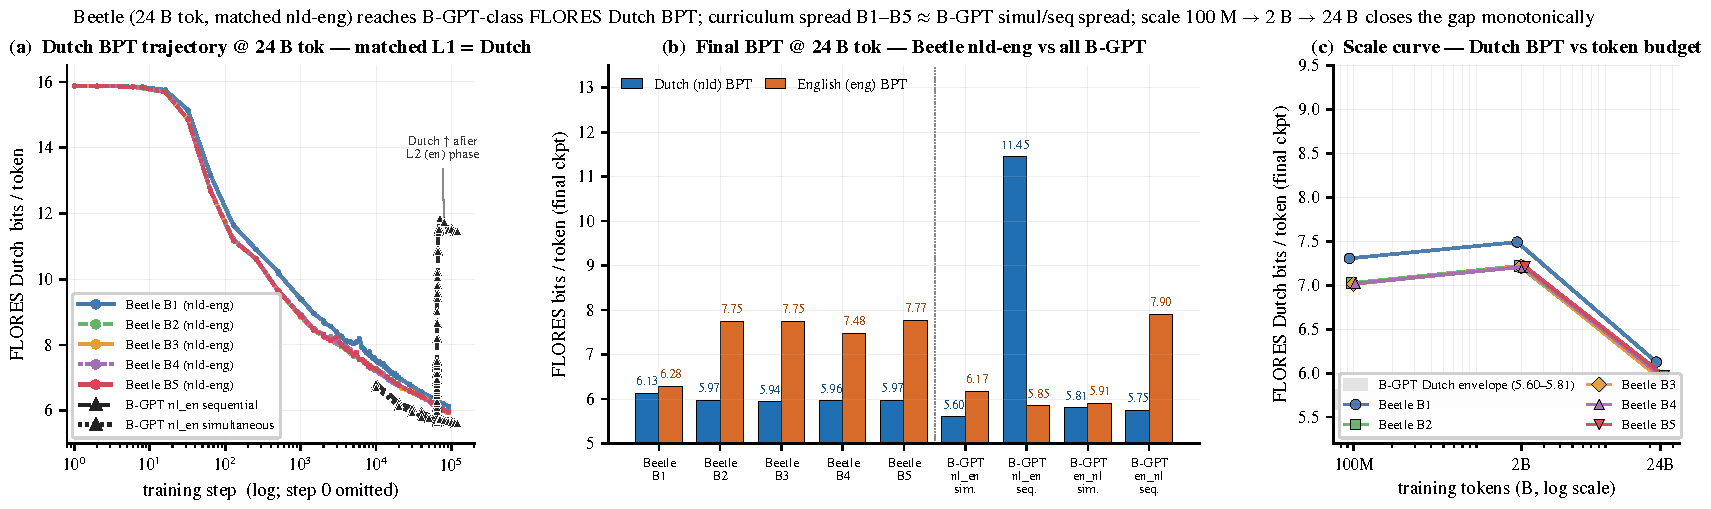
\includegraphics[width=0.86\linewidth,height=0.78\textheight,keepaspectratio]{fig/F10_flores_beetle_vs_bgpt.pdf}
  \caption{FLORES bits-per-byte for matched nld--eng \textsc{Beetle} curricula against B-GPT \citep{arnett-etal-2025-acquisition}: developmental trajectory, final paired bars, and 100M/2B/24B scale curve. Reproduced from main-body Fig.~\ref{fig:flores_beetle_vs_bgpt}.}
  \label{appcomp:F10_flores_beetle_vs_bgpt}
\end{figure*}


\subsection{Per-participant MECO heatmap}


\begin{figure*}[!htbp]
  \centering
  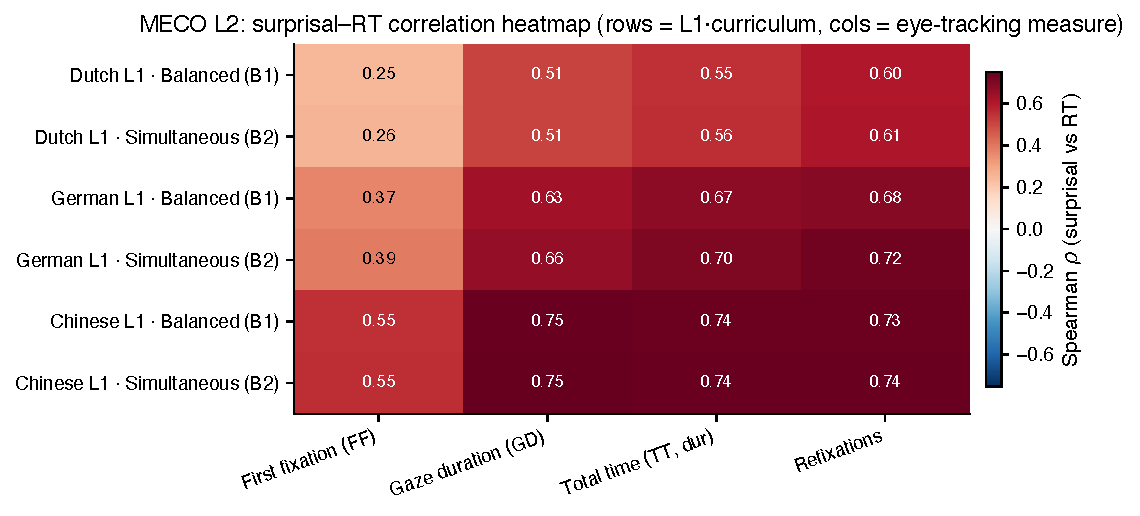
\includegraphics[width=0.86\linewidth,height=0.78\textheight,keepaspectratio]{fig/fig_meco_l2_participants_heatmap.pdf}
  \caption{Per-participant MECO~L2 $\Delta\log L$ heatmap (participant $\times$ model).}
  \label{appcomp:fig_meco_l2_participants_heatmap}
\end{figure*}

\newpage
\subsection{BLiSS supplementary figures}\label{appcomp:bliss}

These figure-set reproductions sit under A.11 (\S\ref{sec:bliss-detail}); they are kept here so the body's cross-figure references resolve to the same physical figure as the in-narrative caption. The cluster anchor \texttt{\textbackslash{}label\{appcomp:bliss\}} is attached above.

\begin{figure}[p]
  \centering
  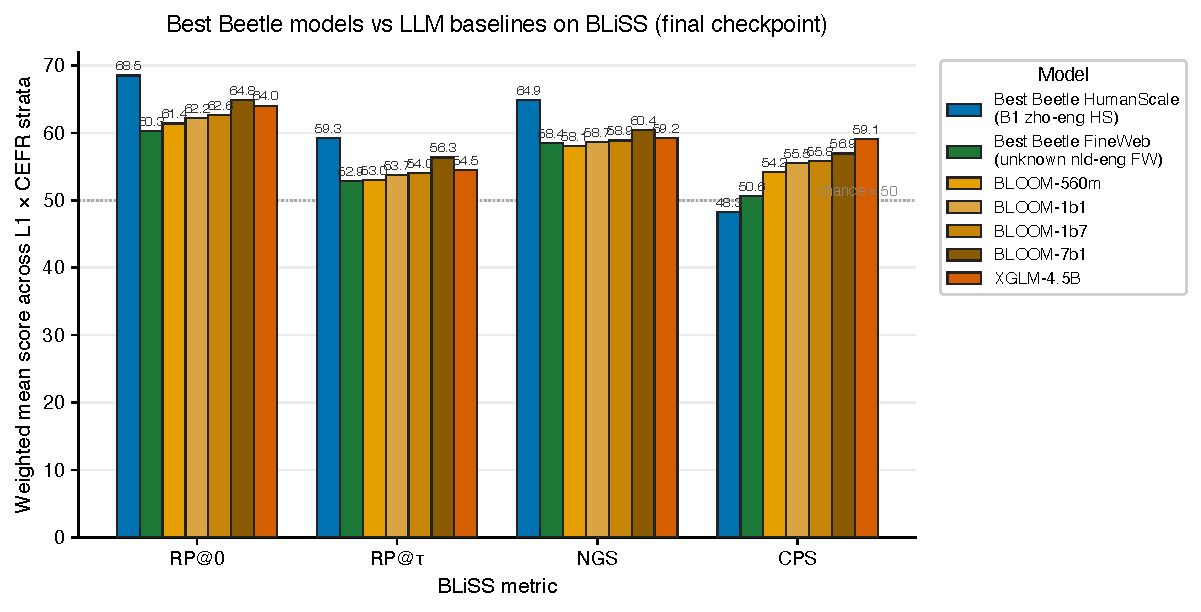
\includegraphics[width=0.86\linewidth,height=0.78\textheight,keepaspectratio]{fig/fig_best_bliss_vs_baselines.pdf}
  \caption{Best \textsc{Beetle} BLiSS NGS (B5 nld--eng \textsc{FineWeb}~2B) against the baseline cohort. Full-resolution reproduction of main-body Fig.~\ref{fig:bliss_best}.}
  \label{appcomp:fig_best_bliss_vs_baselines}
\end{figure}

\begin{figure}[p]
  \centering
  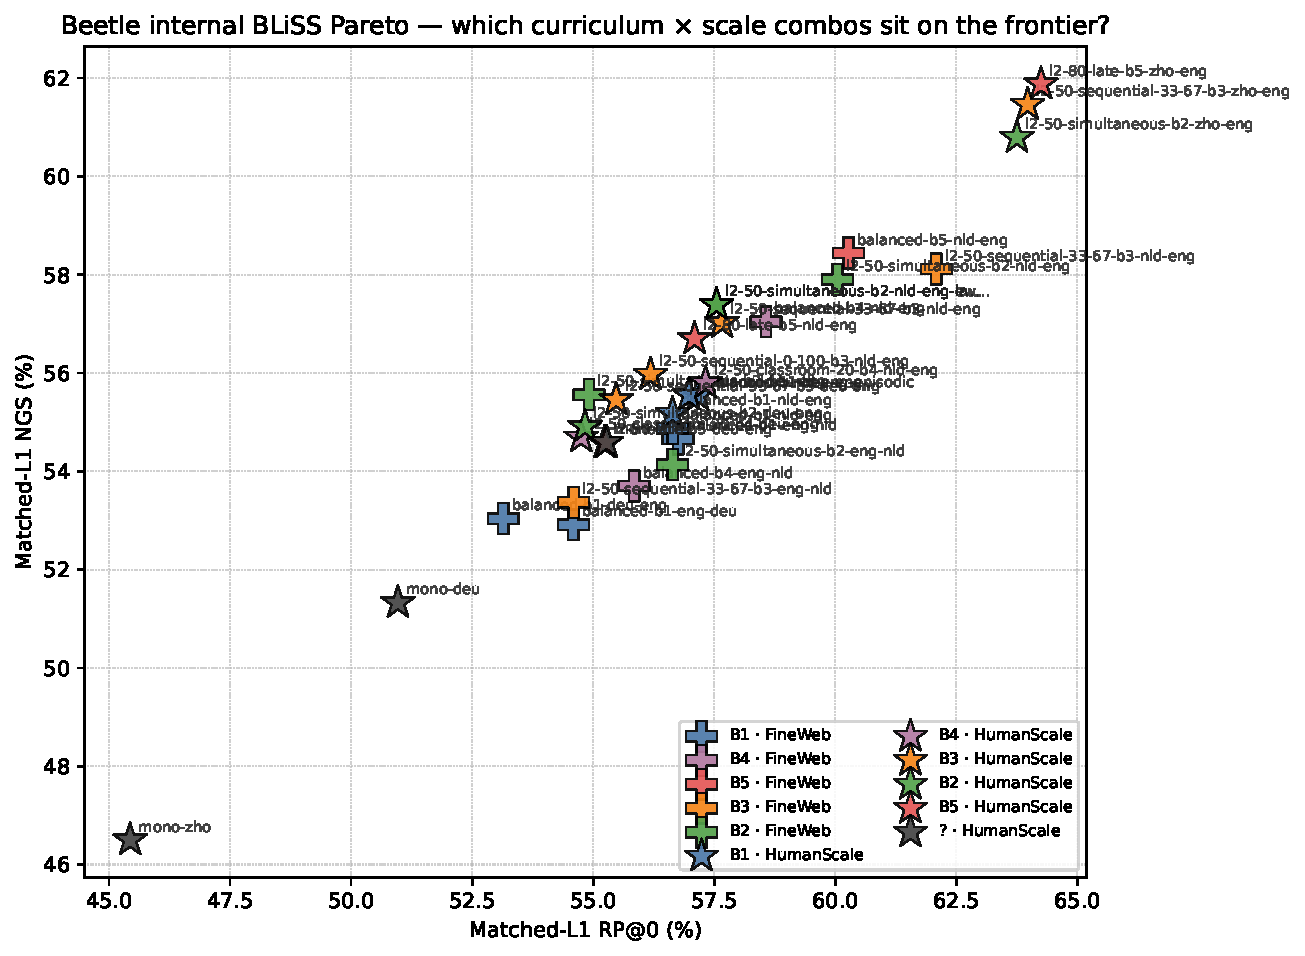
\includegraphics[width=0.86\linewidth,height=0.78\textheight,keepaspectratio]{fig/fig_bliss_beetle_curriculum_frontier.pdf}
  \caption{BLiSS curriculum frontier: NGS as a function of curriculum (B1--B5) at the \textsc{FineWeb}~2B token budget.}
  \label{appcomp:fig_bliss_beetle_curriculum_frontier}
\end{figure}

\begin{figure}[p]
  \centering
  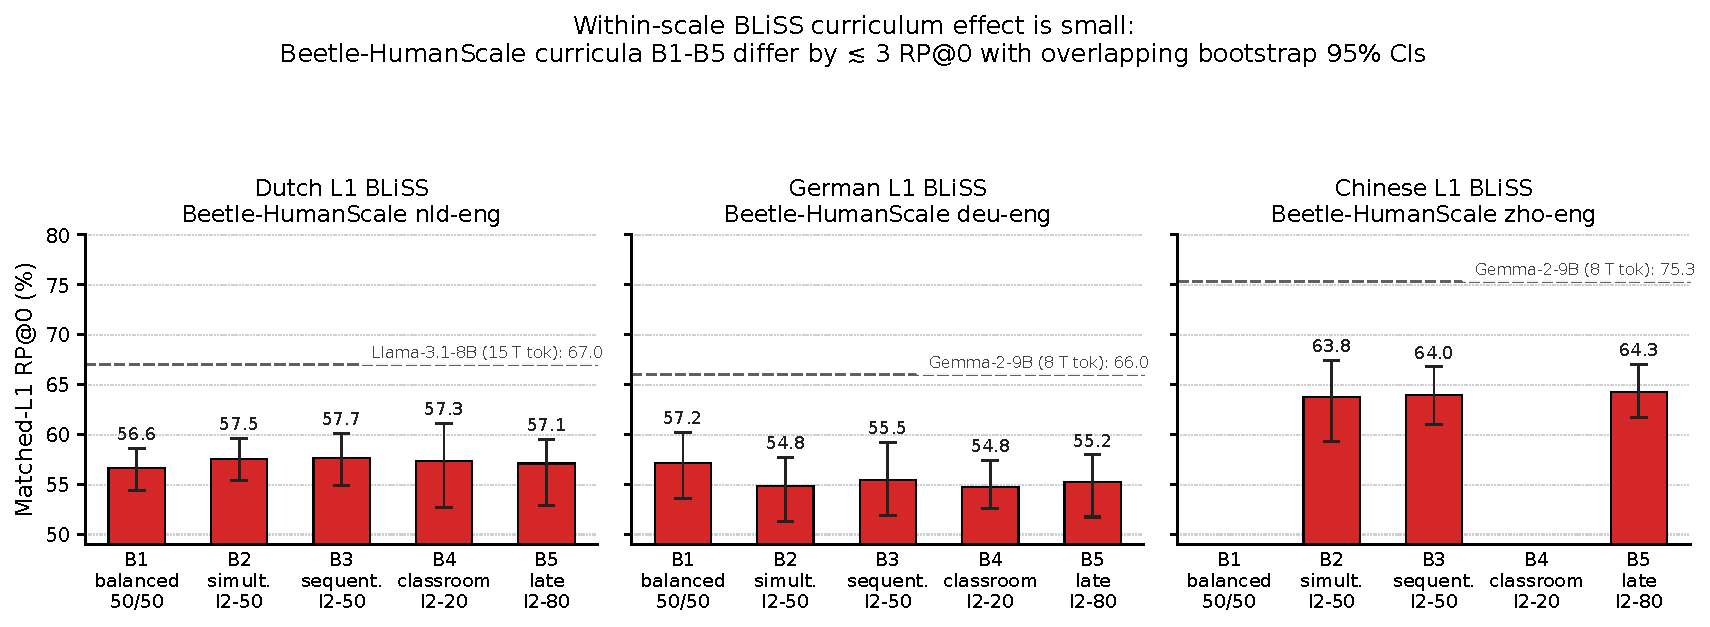
\includegraphics[width=0.86\linewidth,height=0.78\textheight,keepaspectratio]{fig/fig_bliss_curriculum_supp.pdf}
  \caption{Supplementary BLiSS curriculum diagnostics on CPS and RP$@\tau$.}
  \label{appcomp:fig_bliss_curriculum_supp}
\end{figure}

\begin{figure}[p]
  \centering
  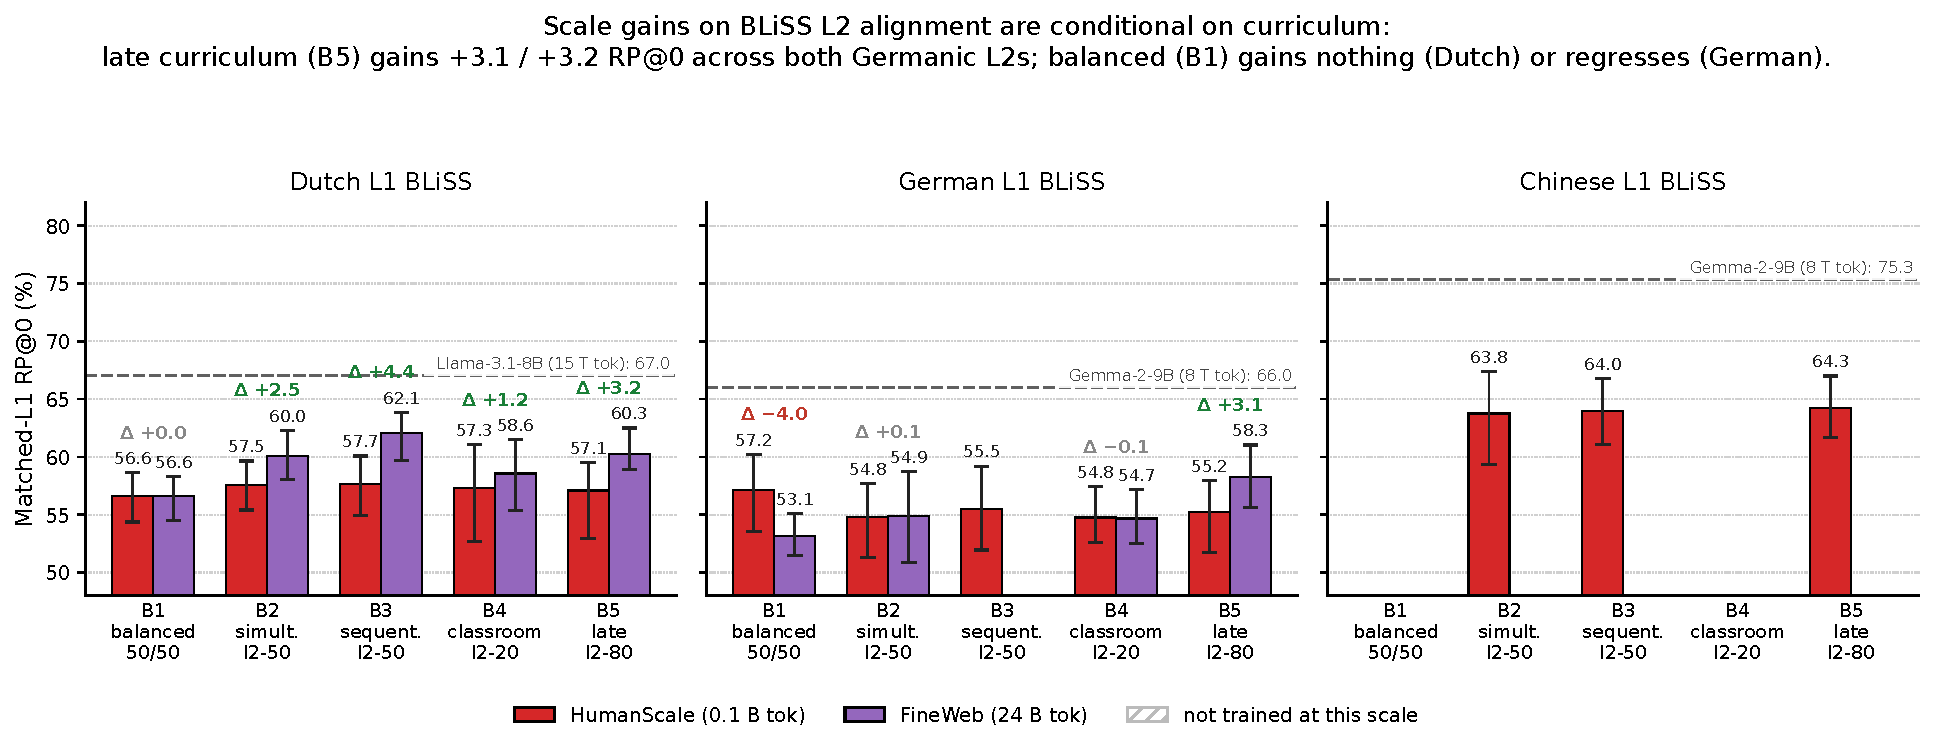
\includegraphics[width=0.86\linewidth,height=0.78\textheight,keepaspectratio]{fig/fig_bliss_main_curriculum.pdf}
  \caption{Aggregated BLiSS NGS by curriculum across all \textsc{Beetle} L1 cohorts.}
  \label{appcomp:fig_bliss_main_curriculum}
\end{figure}

\begin{figure}[p]
  \centering
  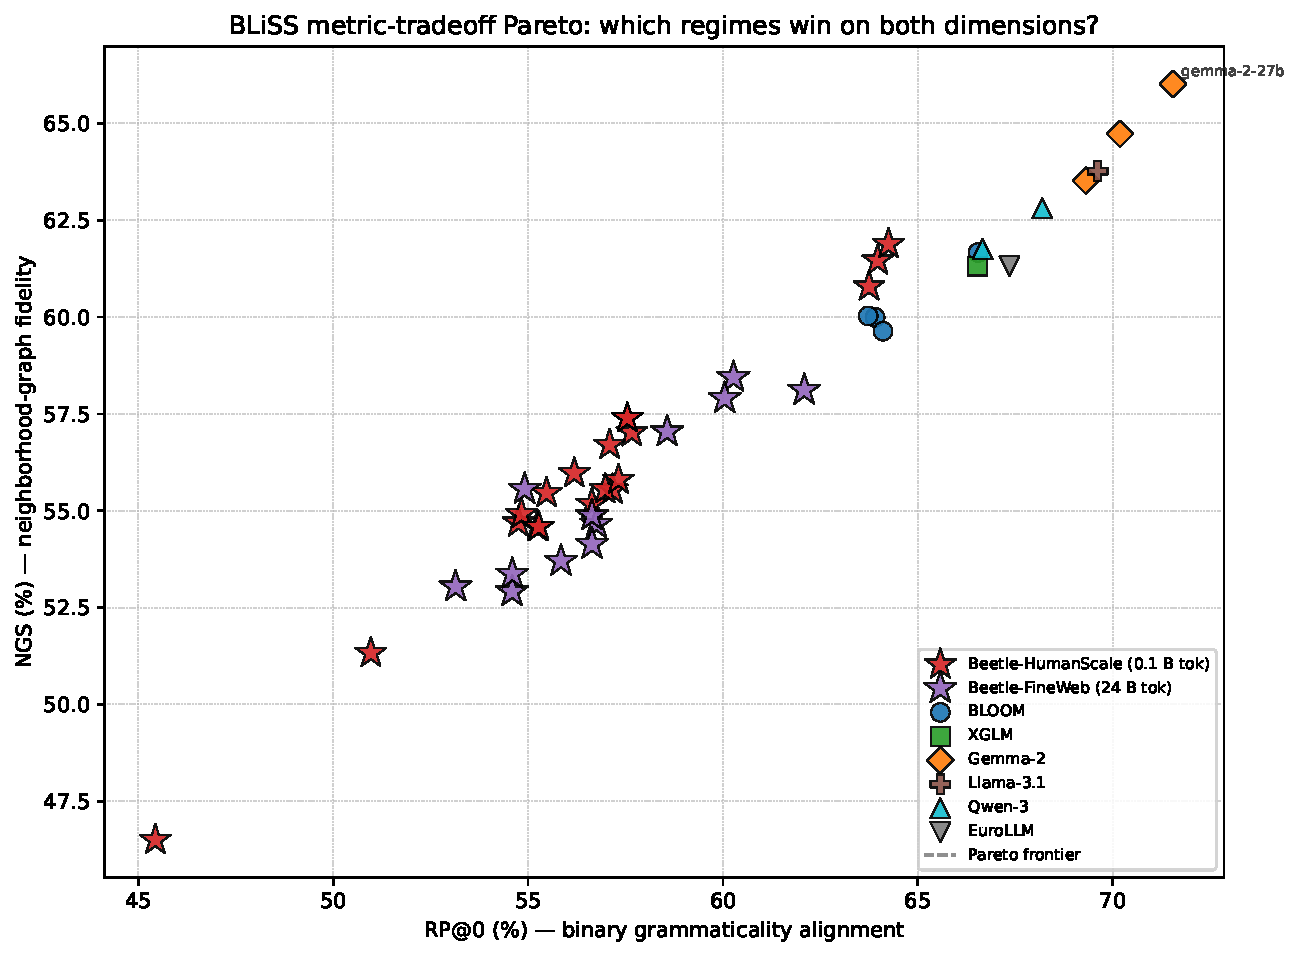
\includegraphics[width=0.86\linewidth,height=0.78\textheight,keepaspectratio]{fig/fig_bliss_pareto_metric_tradeoff.pdf}
  \caption{BLiSS metric trade-off (NGS, CPS, RP$@\tau$); companion to Fig.~\ref{appcomp:F8_bliss_metric_tradeoff_pareto}.}
  \label{appcomp:fig_bliss_pareto_metric_tradeoff}
\end{figure}

\begin{figure}[p]
  \centering
  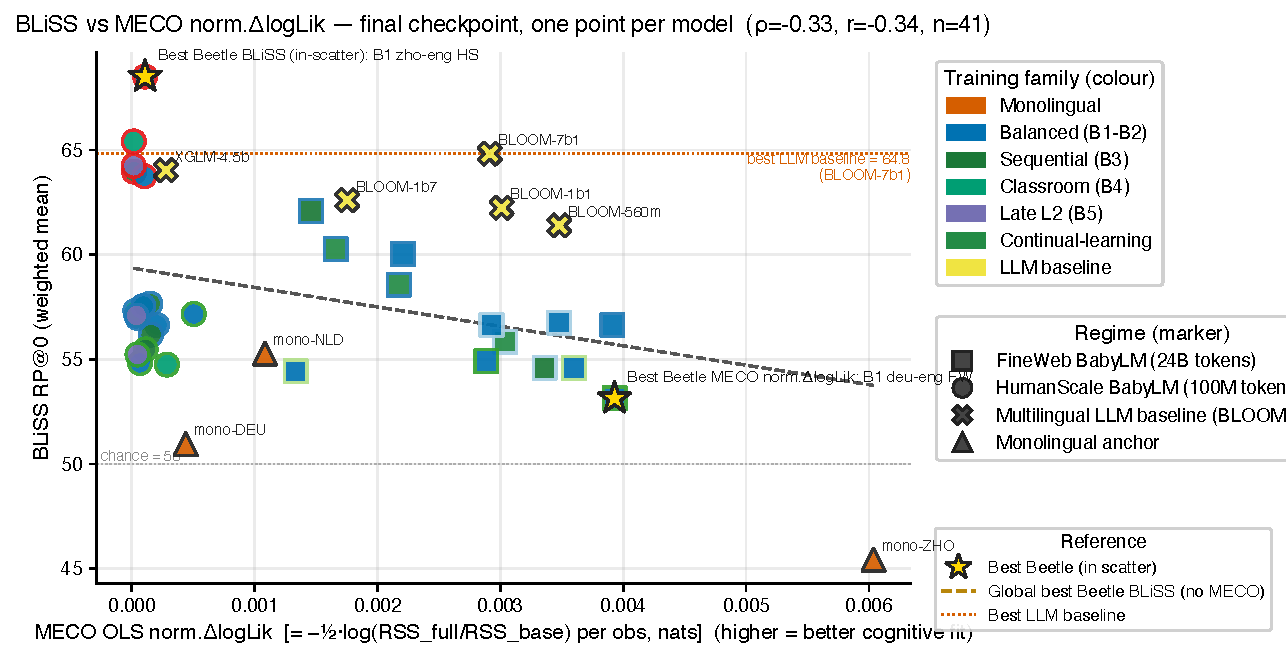
\includegraphics[width=0.86\linewidth,height=0.78\textheight,keepaspectratio]{fig/fig_bliss_vs_meco_final.pdf}
  \caption{Final-checkpoint scatter of BLiSS NGS against MECO~L2 $\Delta\log L$ coloured by curriculum: the curriculum-by-task reordering visualisation underlying \S\ref{sec:pareto}.}
  \label{appcomp:fig_bliss_vs_meco_final}
\end{figure}

\newpage
\subsection{Pedagogical supplementary figures}\label{appcomp:peda}

These pedagogical figure-set reproductions sit under A.12 (\S\ref{sec:pedagogical-detail}); the cluster anchor \texttt{\textbackslash{}label\{appcomp:peda\}} is attached above so body references can point at the whole figure group with one ref.

\begin{figure}[p]
  \centering
  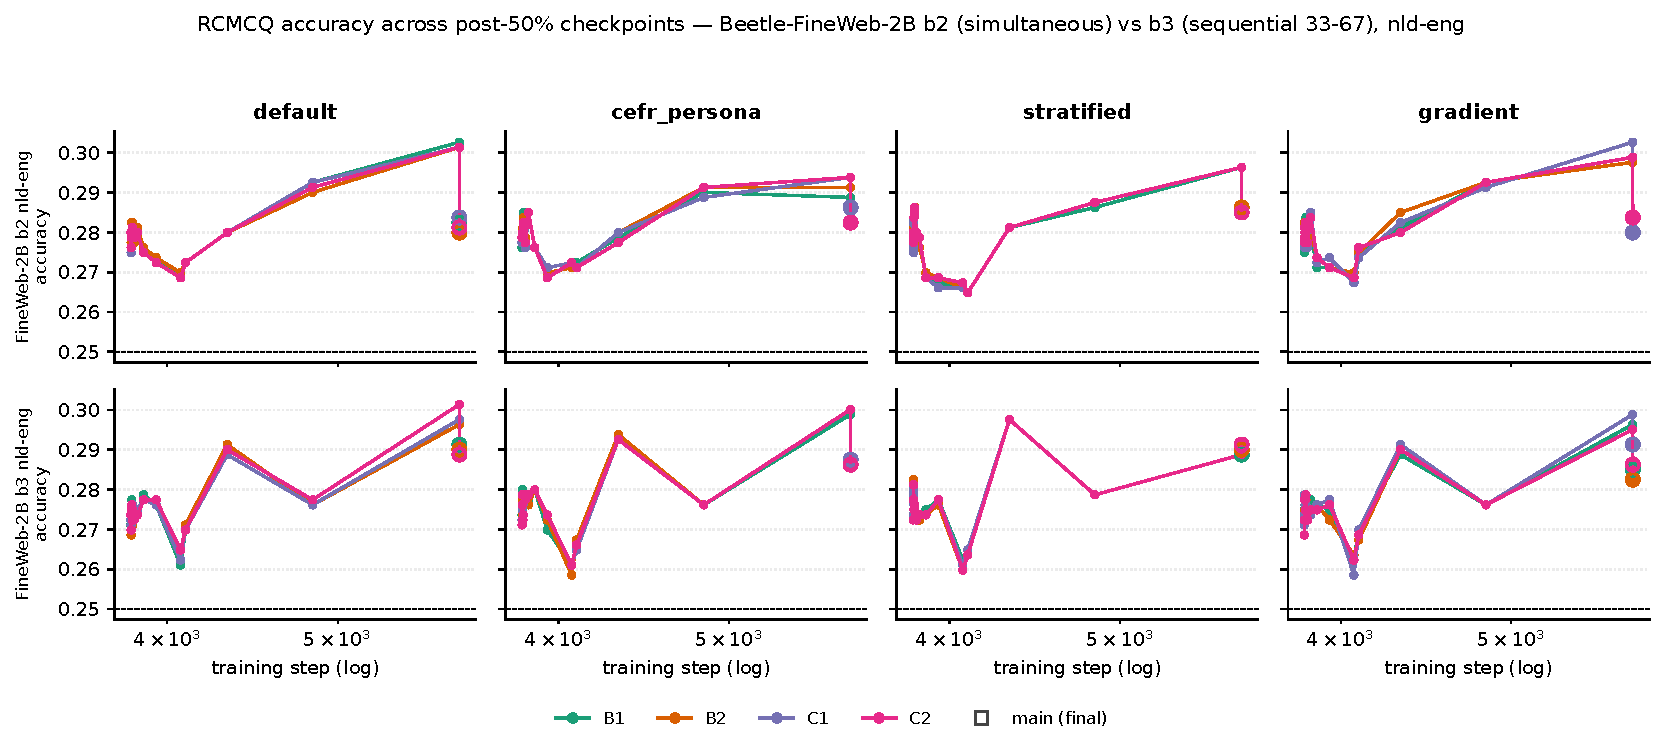
\includegraphics[width=0.86\linewidth,height=0.78\textheight,keepaspectratio]{fig/figC_ckpt_rcmcq_trace.pdf}
  \caption{Reading-comprehension multiple-choice accuracy trace across log-spaced 24B-token \textsc{Beetle} checkpoints.}
  \label{appcomp:figC_ckpt_rcmcq_trace}
\end{figure}

% Composite pedagogical-utility figure (figC_pedagogical_utility.pdf) and
% the headline_pedagogical_2x2.pdf grid have been pulled from the appendix
% figure set. Both renders contain an EVP-acquisition panel that is not
% load-bearing on any body claim: the EVP-acquisition trajectory is not
% reproducible from the committed analysis bundle (see App.~\ref{sec:roadmap}
% item~\ref{item:evp-trajectory-recompute}) and has been dropped from the body
% pedagogical axis list (\S\ref{sec:discrimination}). The CUP\&A5 / CLOTH /
% JFLEG components remain available individually via the released CSVs and the
% per-axis figures retained below; the composite renders will be regenerated
% without the EVP panel for the camera-ready.

\begin{figure}[p]
  \centering
  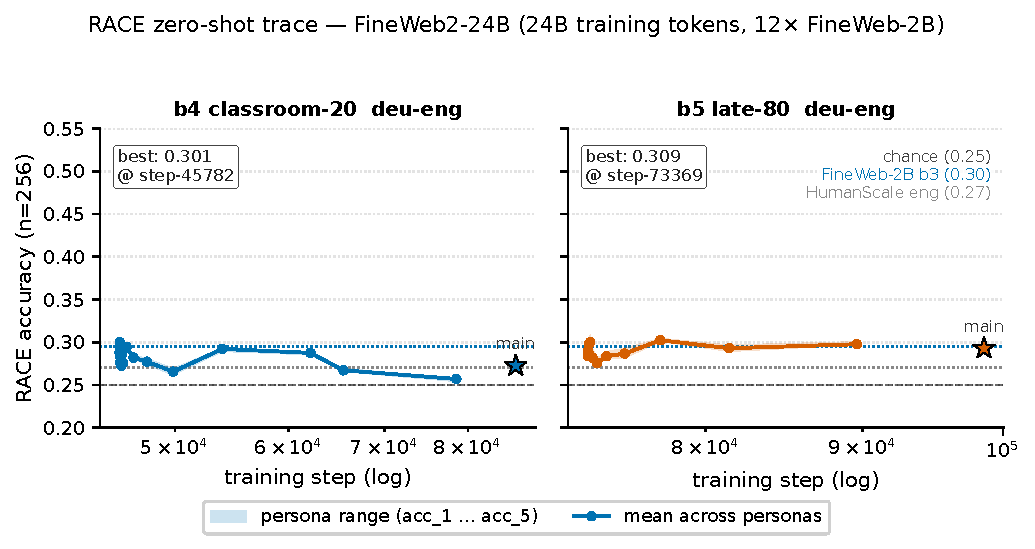
\includegraphics[width=0.86\linewidth,height=0.78\textheight,keepaspectratio]{fig/figC_race_24b_trace.pdf}
  \caption{RACE zero-shot accuracy trace across 24B-token \textsc{Beetle} checkpoints (pre-fine-tuning baseline).}
  \label{appcomp:figC_race_24b_trace}
\end{figure}

\begin{figure}[p]
  \centering
  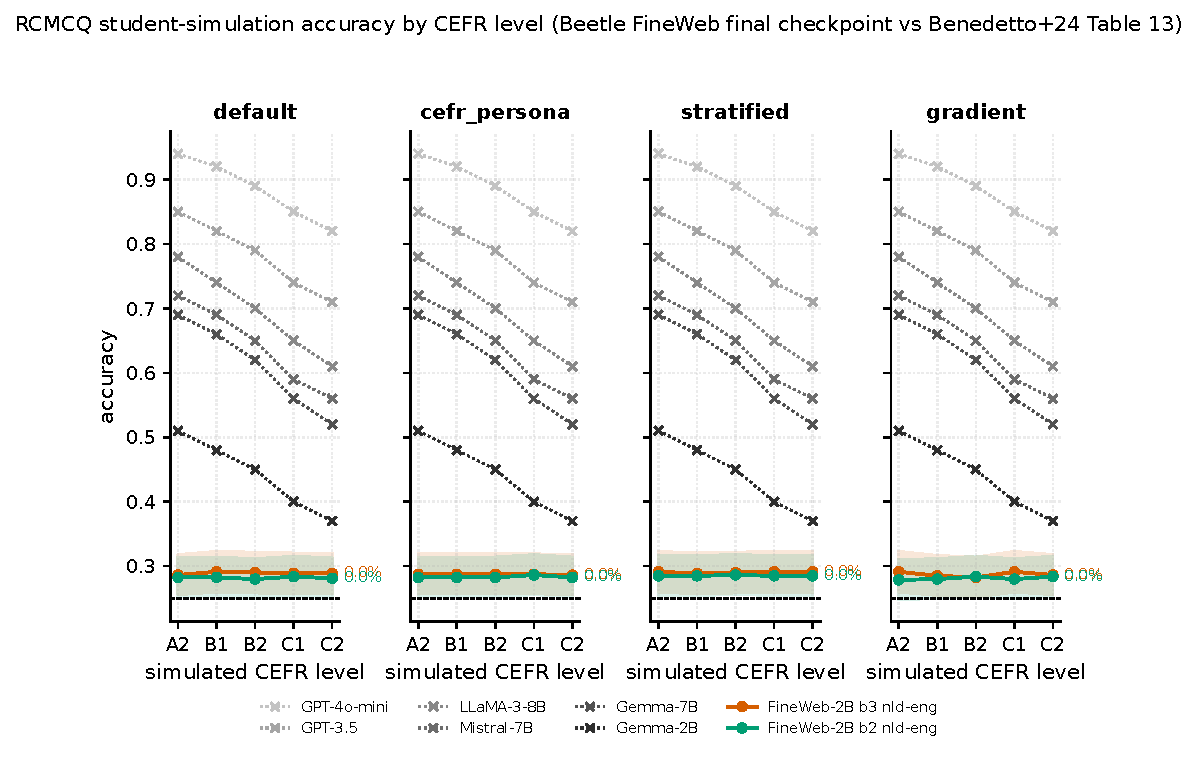
\includegraphics[width=0.86\linewidth,height=0.78\textheight,keepaspectratio]{fig/figC_rcmcq_cefr.pdf}
  \caption{CEFR-stratified reading-comprehension multiple-choice accuracy across the four prompting variants of CUP\&A5.}
  \label{appcomp:figC_rcmcq_cefr}
\end{figure}

\begin{figure}[p]
  \centering
  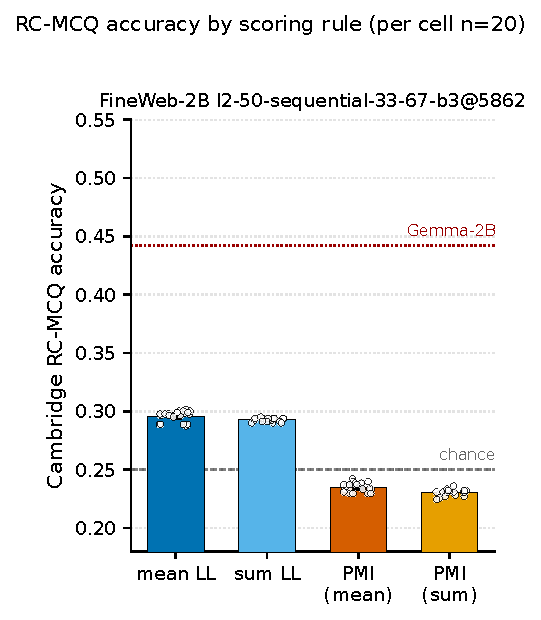
\includegraphics[width=0.86\linewidth,height=0.78\textheight,keepaspectratio]{fig/figC_score_variants.pdf}
  \caption{Score-variant ablation for the CUP\&A5 reading-comprehension task across normalisation choices.}
  \label{appcomp:figC_score_variants}
\end{figure}

\begin{figure}[p]
  \centering
  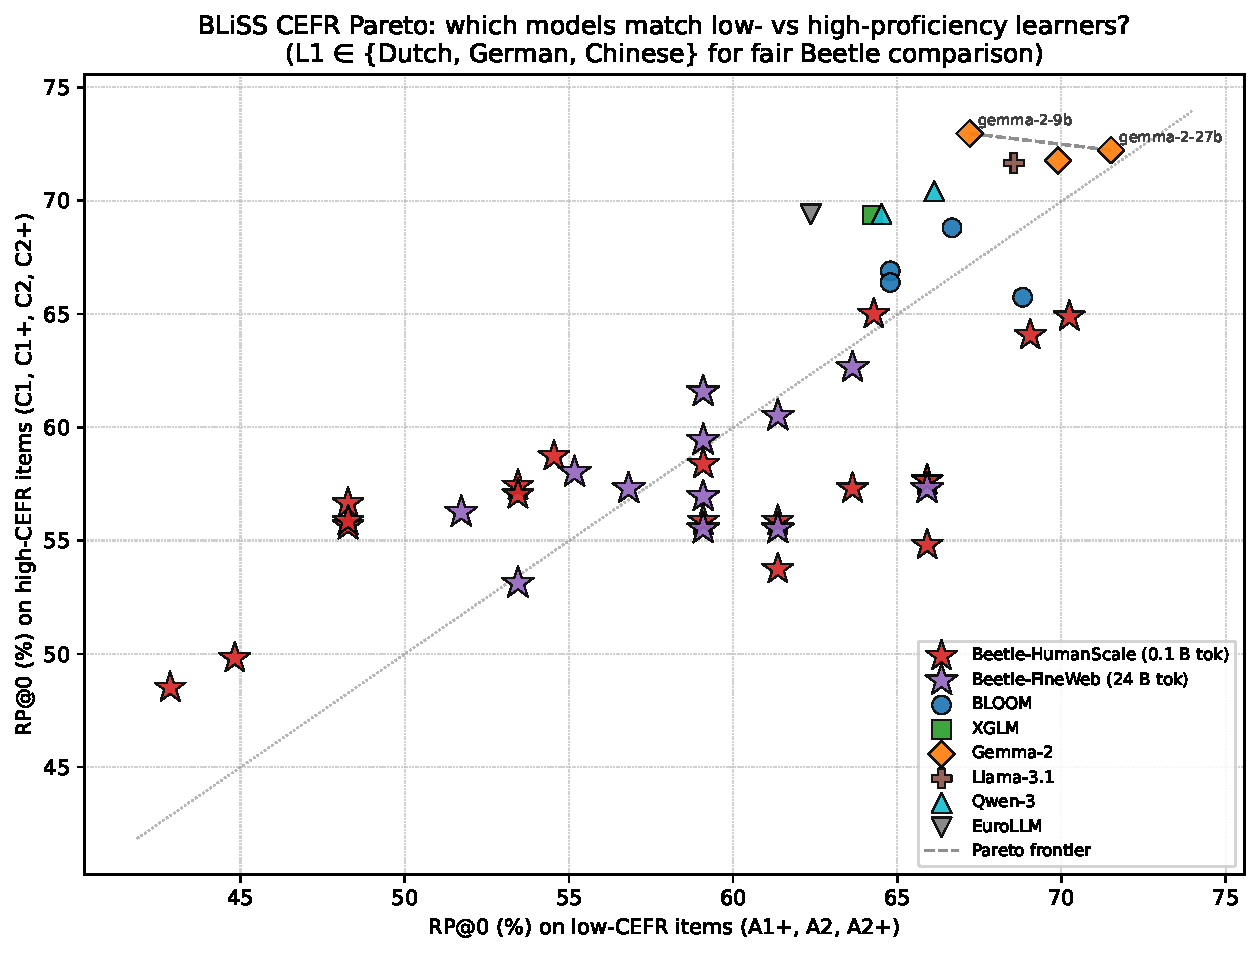
\includegraphics[width=0.86\linewidth,height=0.78\textheight,keepaspectratio]{fig/fig_bliss_pareto_cefr.pdf}
  \caption{BLiSS curriculum spread cross-referenced against CEFR difficulty stratification.}
  \label{appcomp:fig_bliss_pareto_cefr}
\end{figure}

% See the joint EVP-residue note immediately preceding
% \ref{appcomp:figC_race_24b_trace} for the disposition of
% headline_pedagogical_2x2.pdf (held back together with
% figC_pedagogical_utility.pdf pending the EVP-stripped re-render).

\begin{figure}[p]
  \centering
  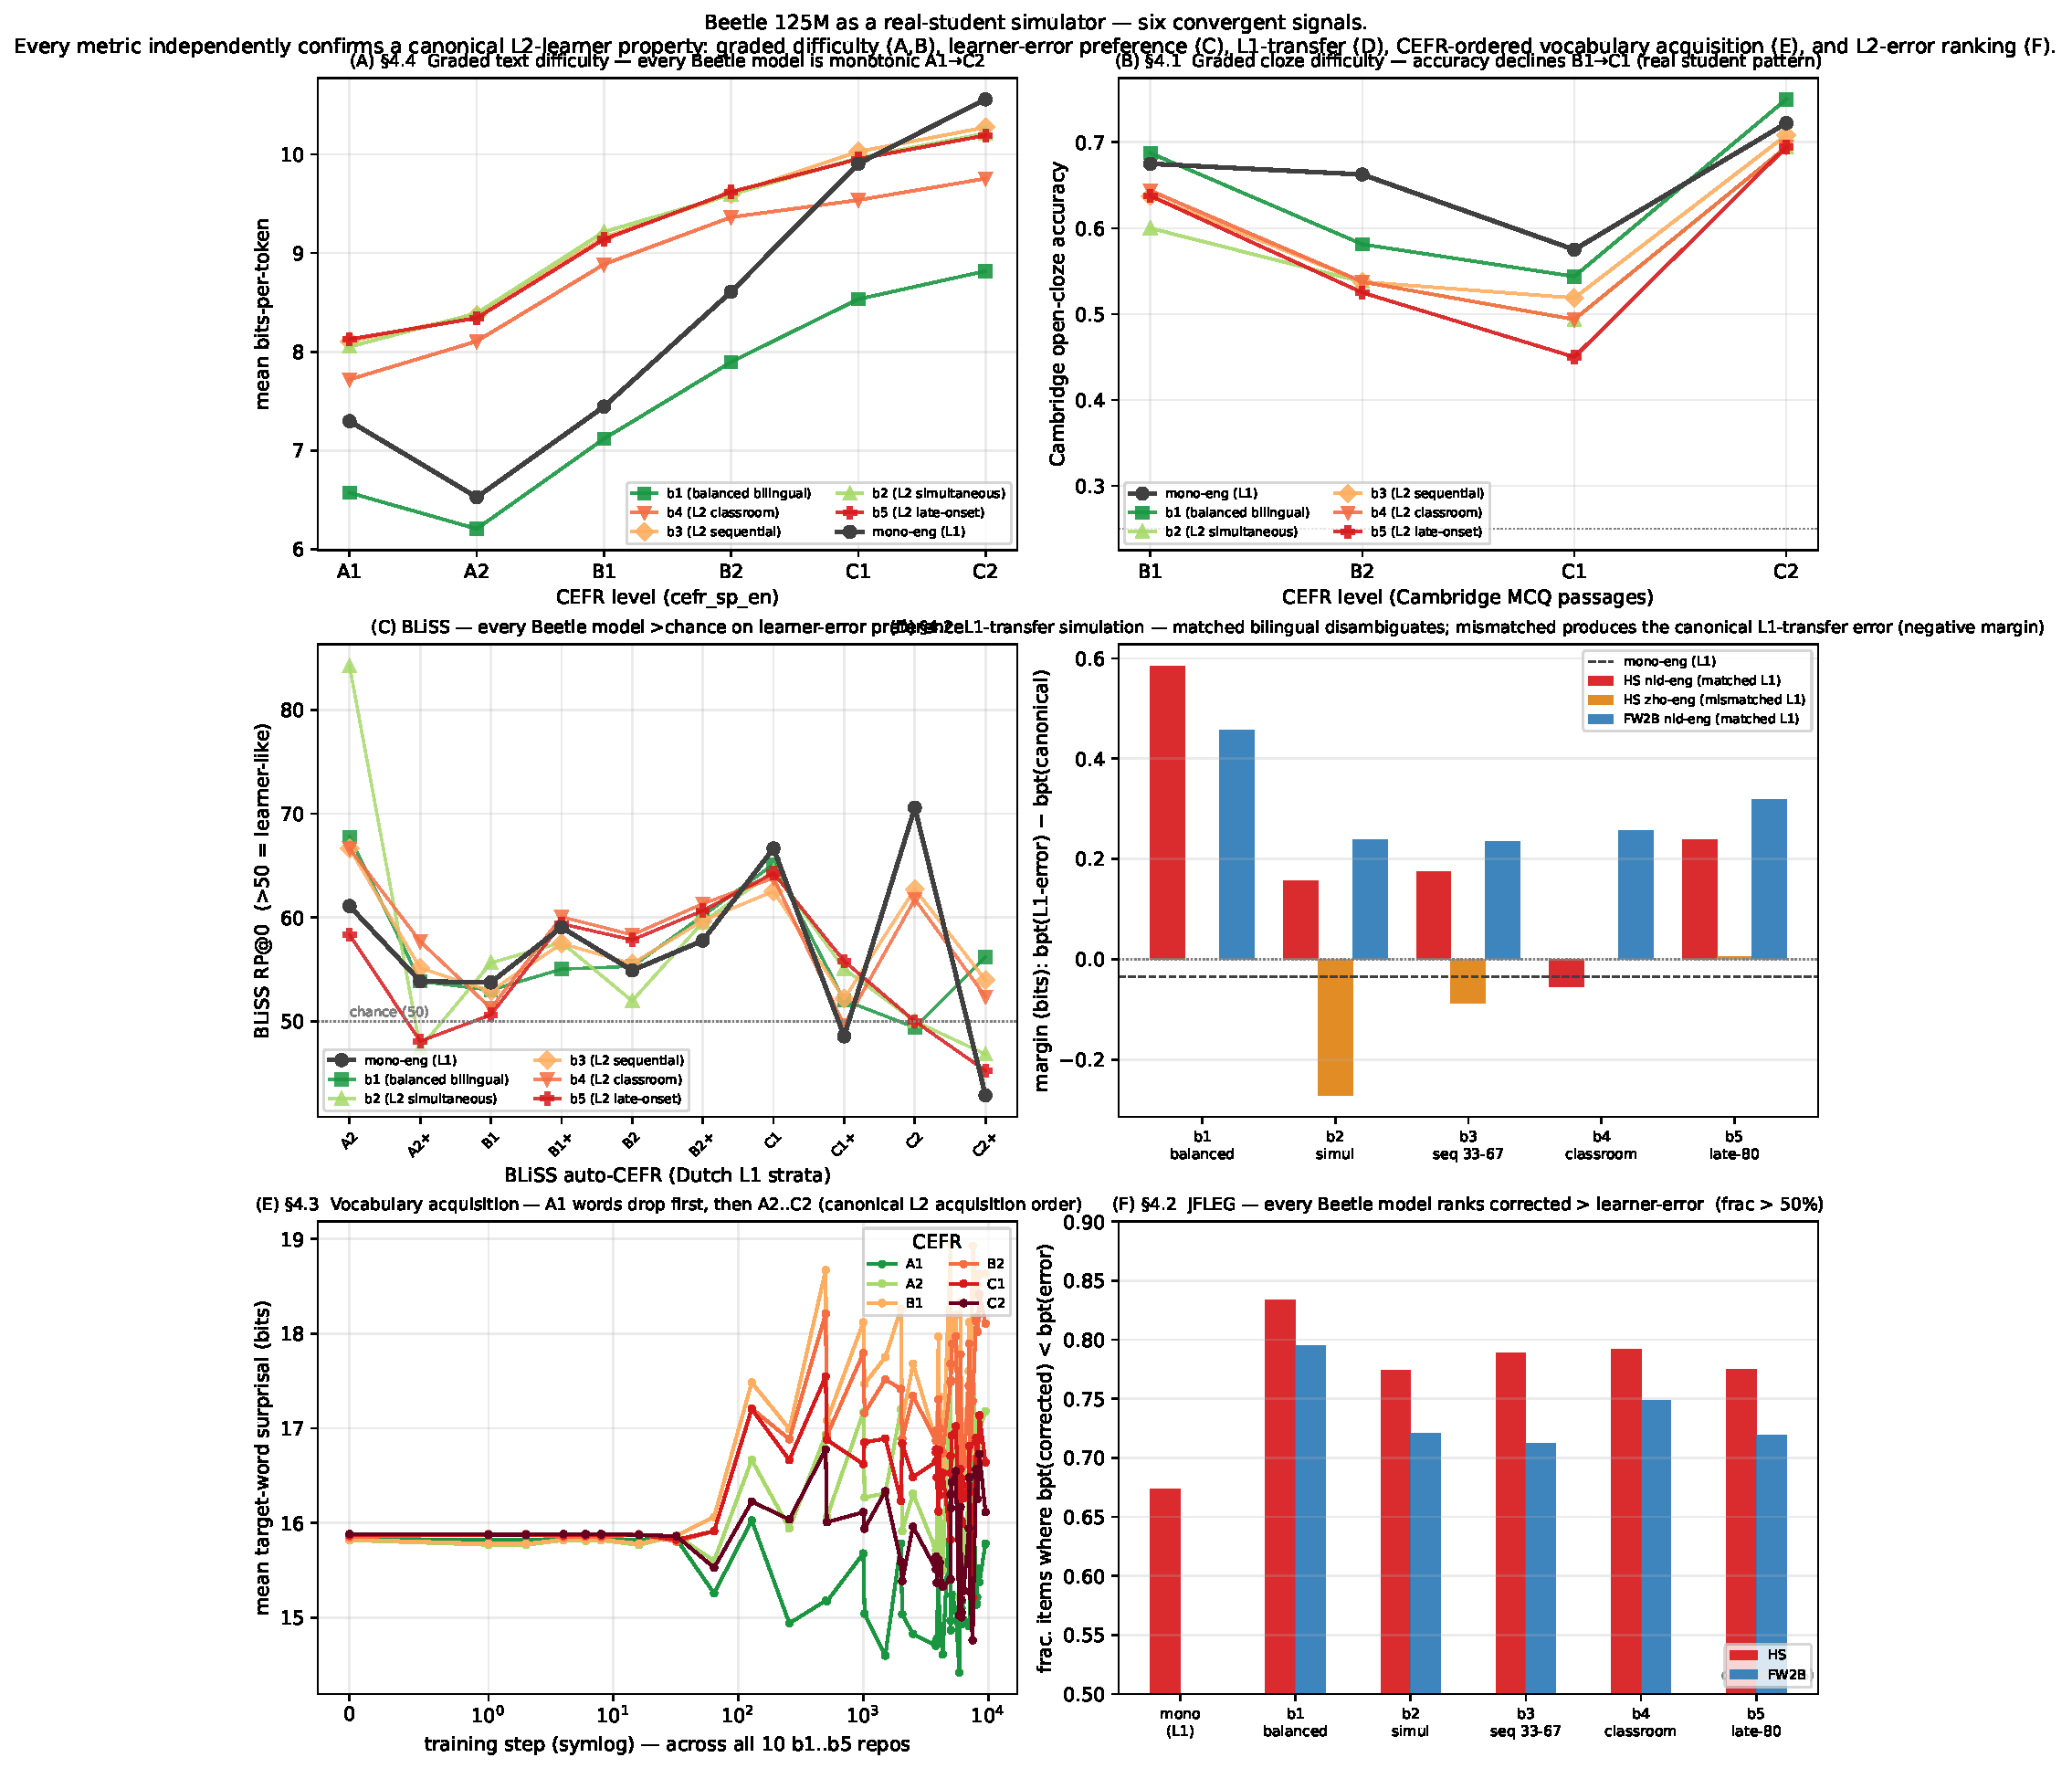
\includegraphics[width=0.86\linewidth,height=0.78\textheight,keepaspectratio]{fig/headline_pedagogical_evidence.pdf}
  \caption{Consolidated pedagogical-evidence panel; companion to body Tab.~\ref{tab:headline_pedagogical}.}
  \label{appcomp:headline_pedagogical_evidence}
\end{figure}

\begin{figure}[p]
  \centering
  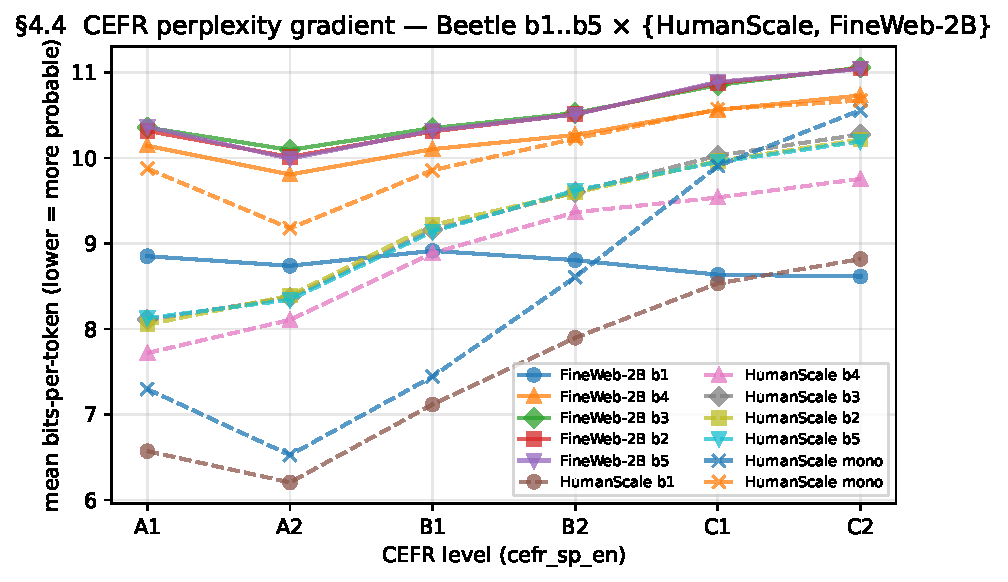
\includegraphics[width=0.86\linewidth,height=0.78\textheight,keepaspectratio]{fig/panelA_cefr_ppl_gradient.pdf}
  \caption{CEFR perplexity gradient (A1--C2) for \textsc{Beetle} curricula and the baseline cohort.}
  \label{appcomp:panelA_cefr_ppl_gradient}
\end{figure}

\begin{figure}[p]
  \centering
  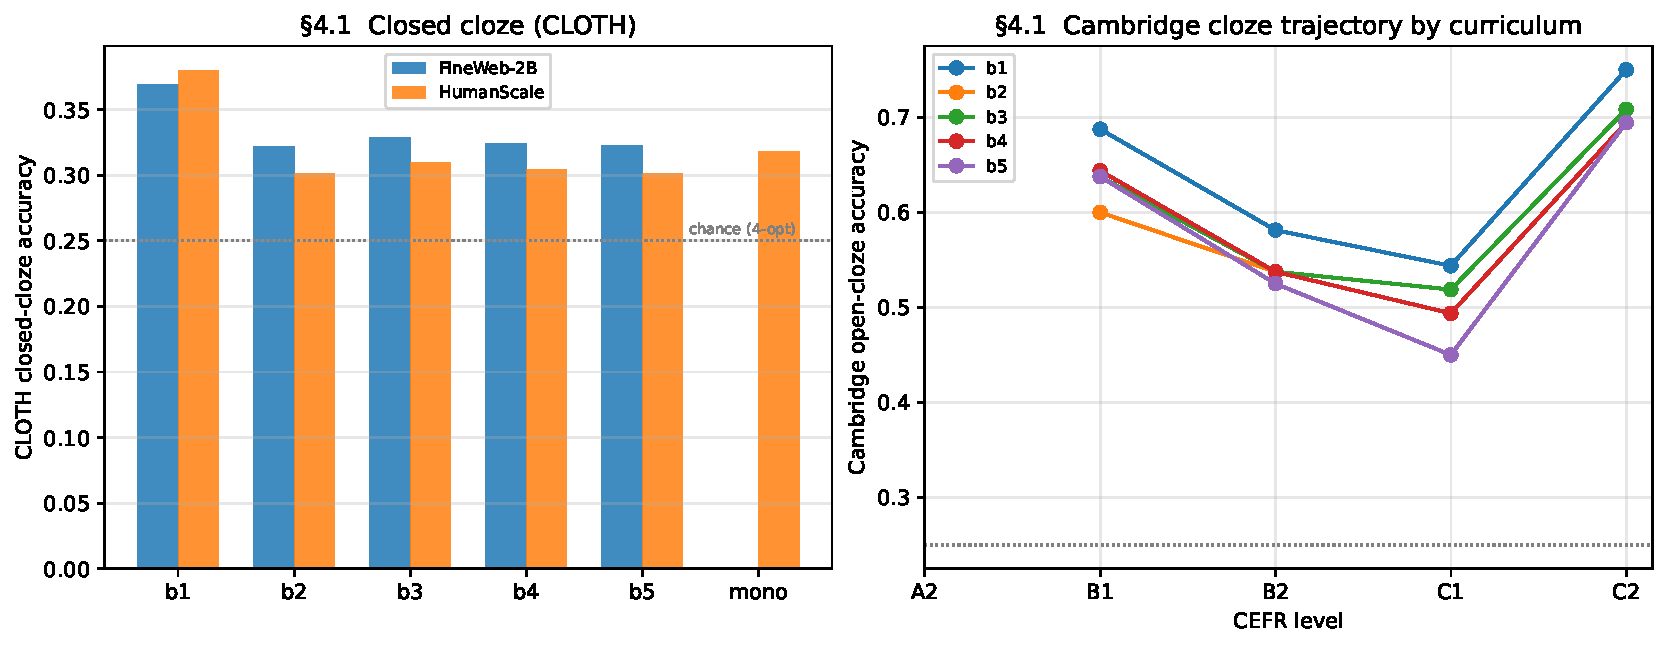
\includegraphics[width=0.86\linewidth,height=0.78\textheight,keepaspectratio]{fig/panelB_cloze.pdf}
  \caption{CLOTH closed-cloze accuracy by CEFR level for \textsc{Beetle} curricula.}
  \label{appcomp:panelB_cloze}
\end{figure}

\begin{figure}[p]
  \centering
  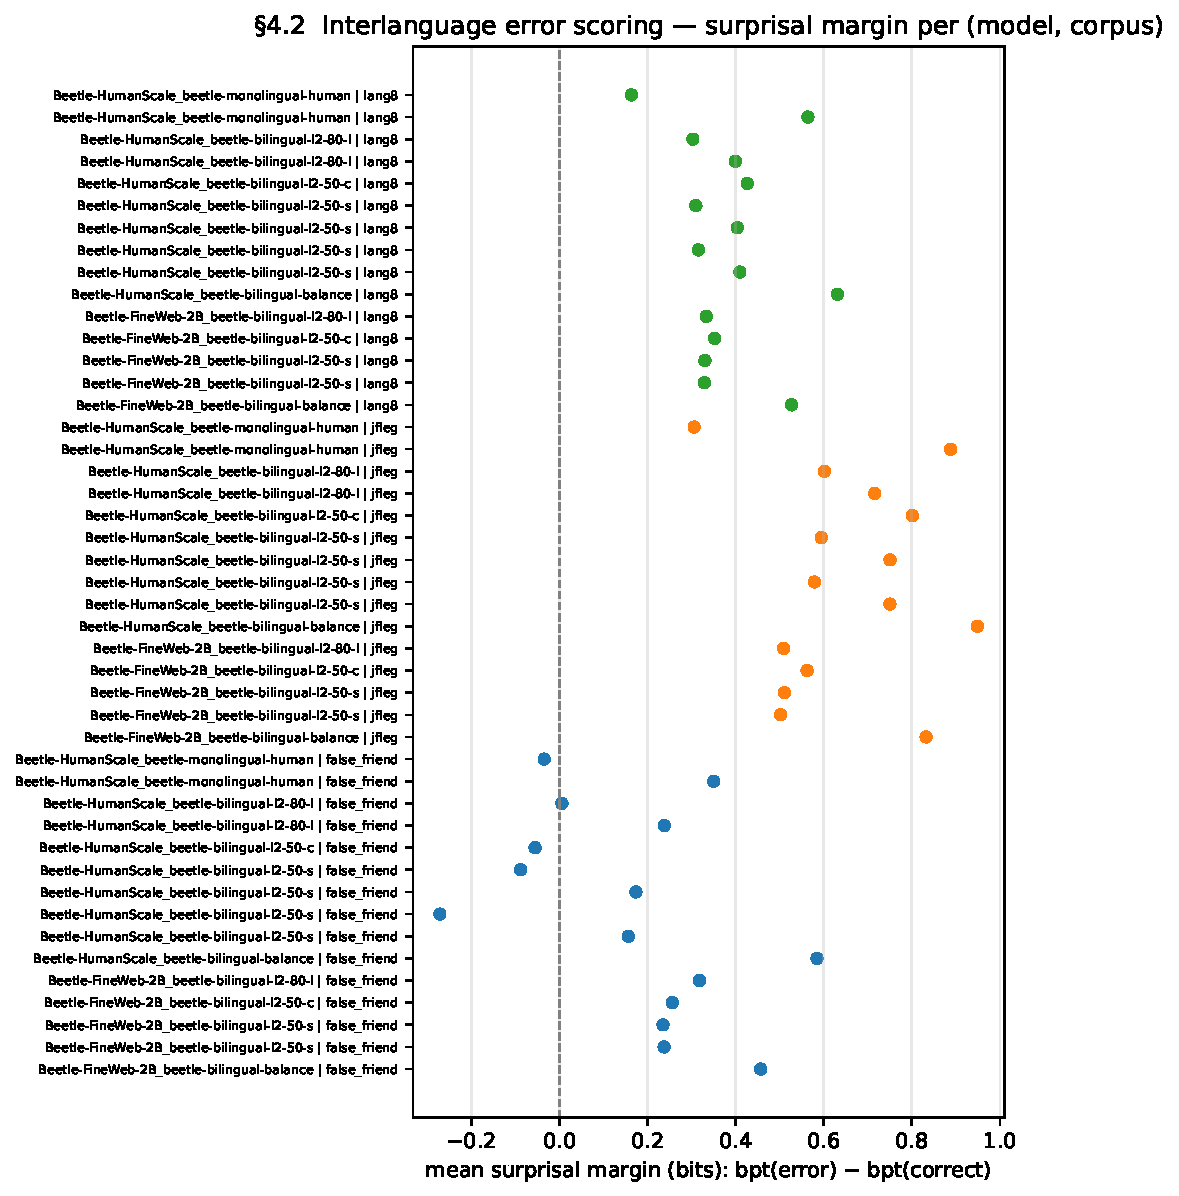
\includegraphics[width=0.86\linewidth,height=0.78\textheight,keepaspectratio]{fig/panelC_interlanguage_forest.pdf}
  \caption{Interlanguage error-discrimination forest plot for the pedagogical evaluation cohort.}
  \label{appcomp:panelC_interlanguage_forest}
\end{figure}


\begin{figure}[p]
  \centering
  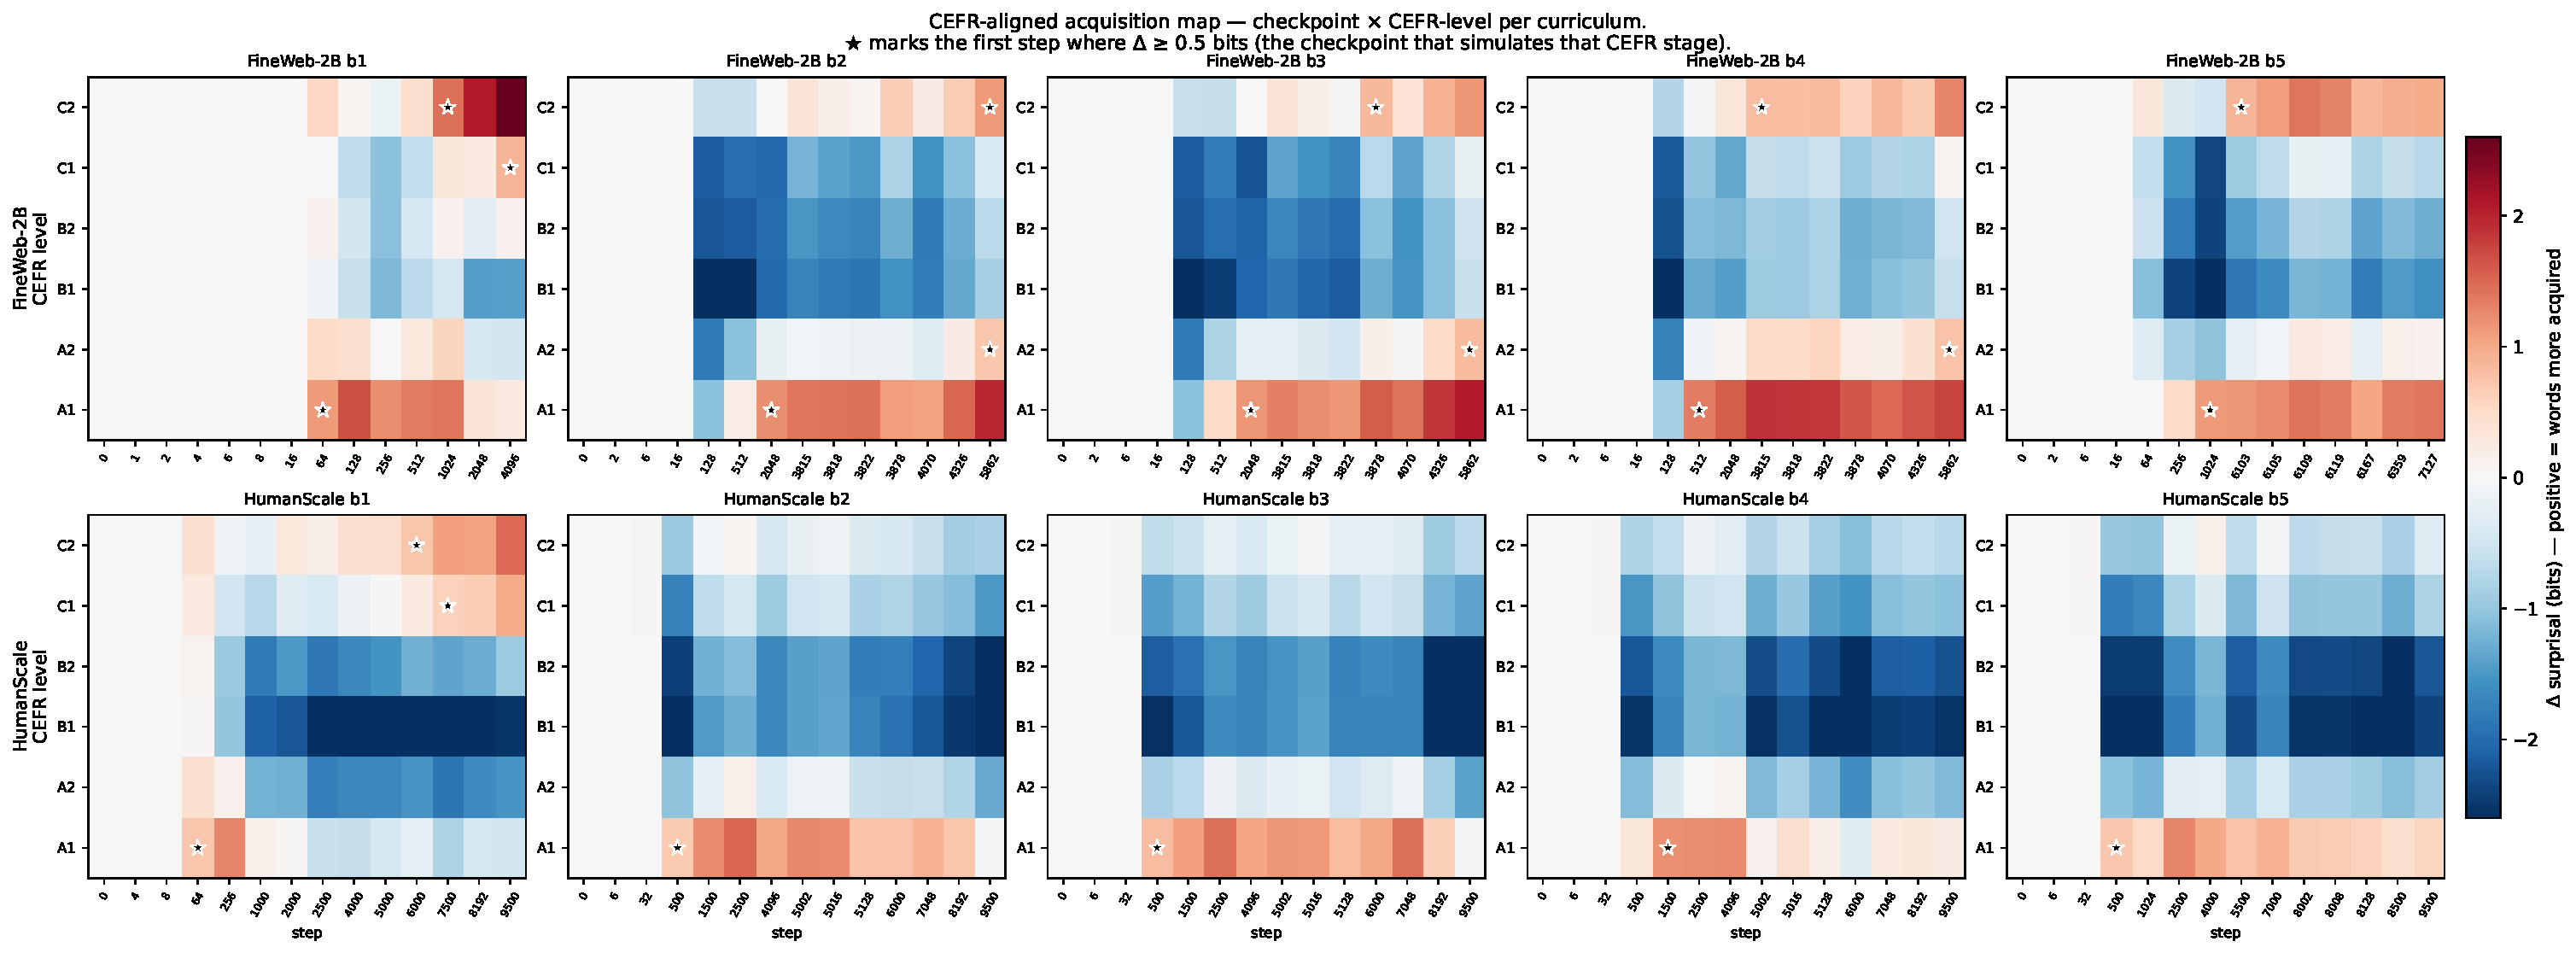
\includegraphics[width=0.86\linewidth,height=0.78\textheight,keepaspectratio]{fig/trajectory_cefr_alignment_heatmap.pdf}
  \caption{CEFR alignment heatmap: levels A1--C2 against log-spaced training step for the B3-33 nld--eng \textsc{Beetle} run.}
  \label{appcomp:trajectory_cefr_alignment_heatmap}
\end{figure}

\begin{figure}[p]
  \centering
  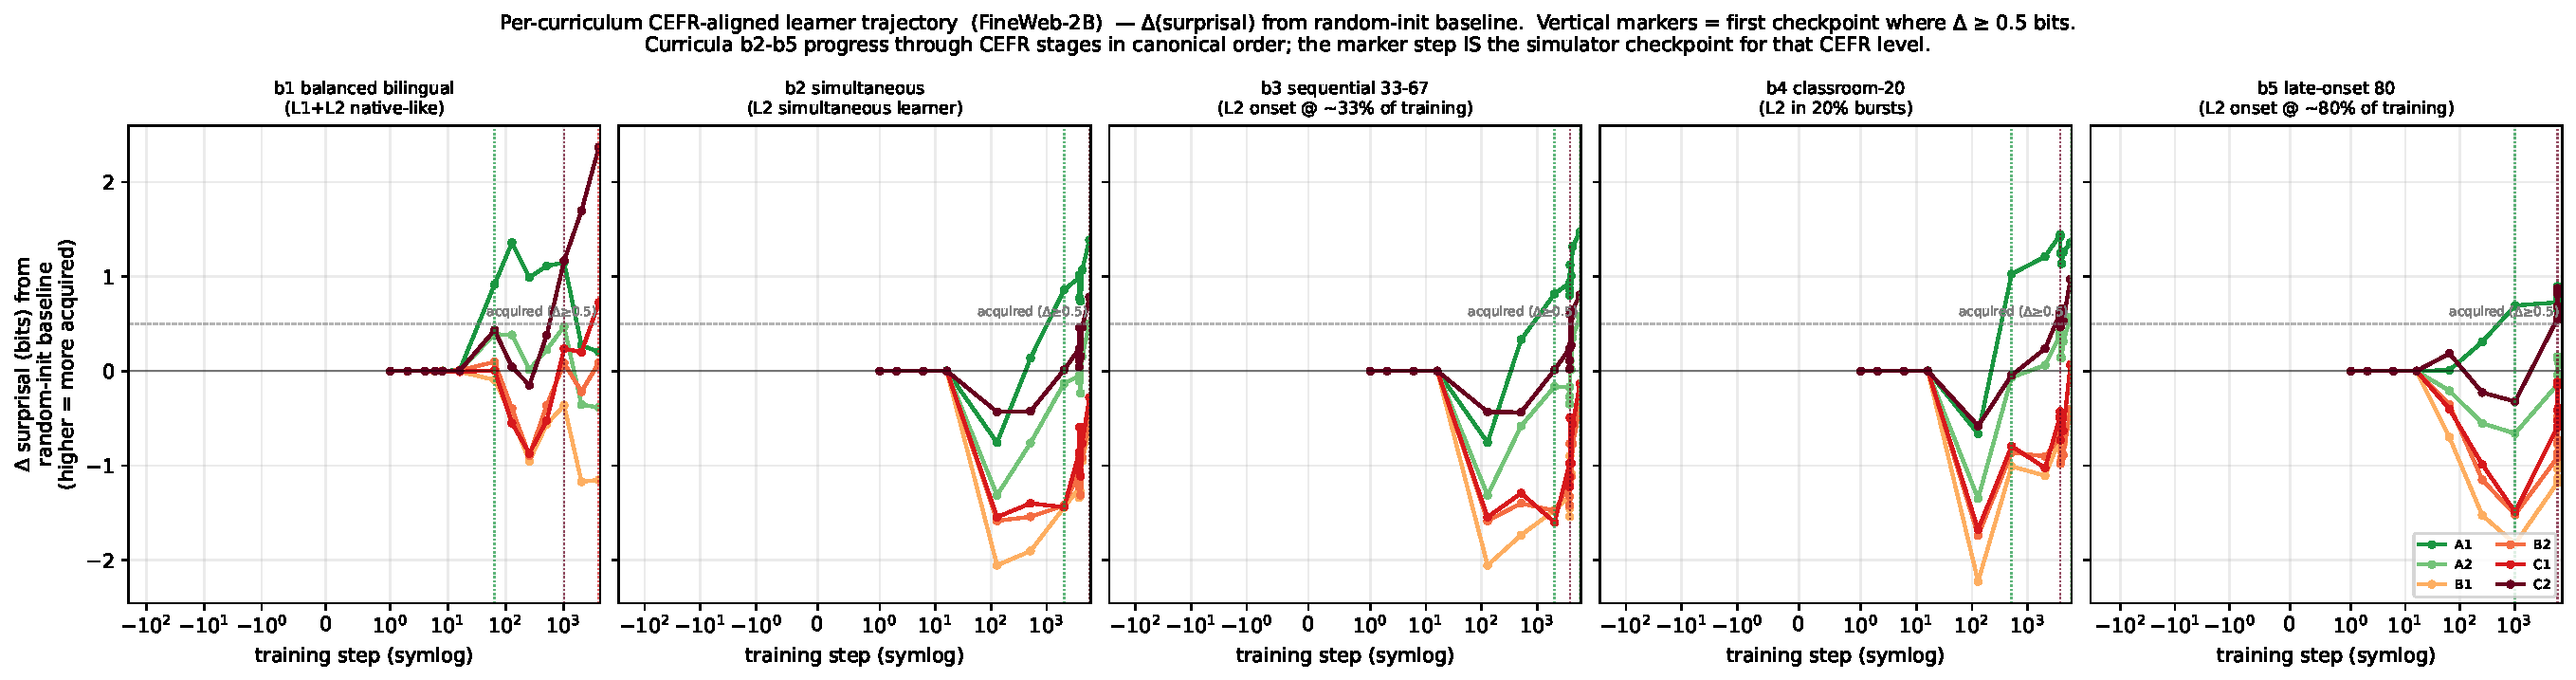
\includegraphics[width=0.86\linewidth,height=0.78\textheight,keepaspectratio]{fig/trajectory_cefr_fineweb2b.pdf}
  \caption{CEFR alignment trajectory at the \textsc{FineWeb}~2B token budget for \textsc{Beetle} curricula.}
  \label{appcomp:trajectory_cefr_fineweb2b}
\end{figure}

\begin{figure}[p]
  \centering
  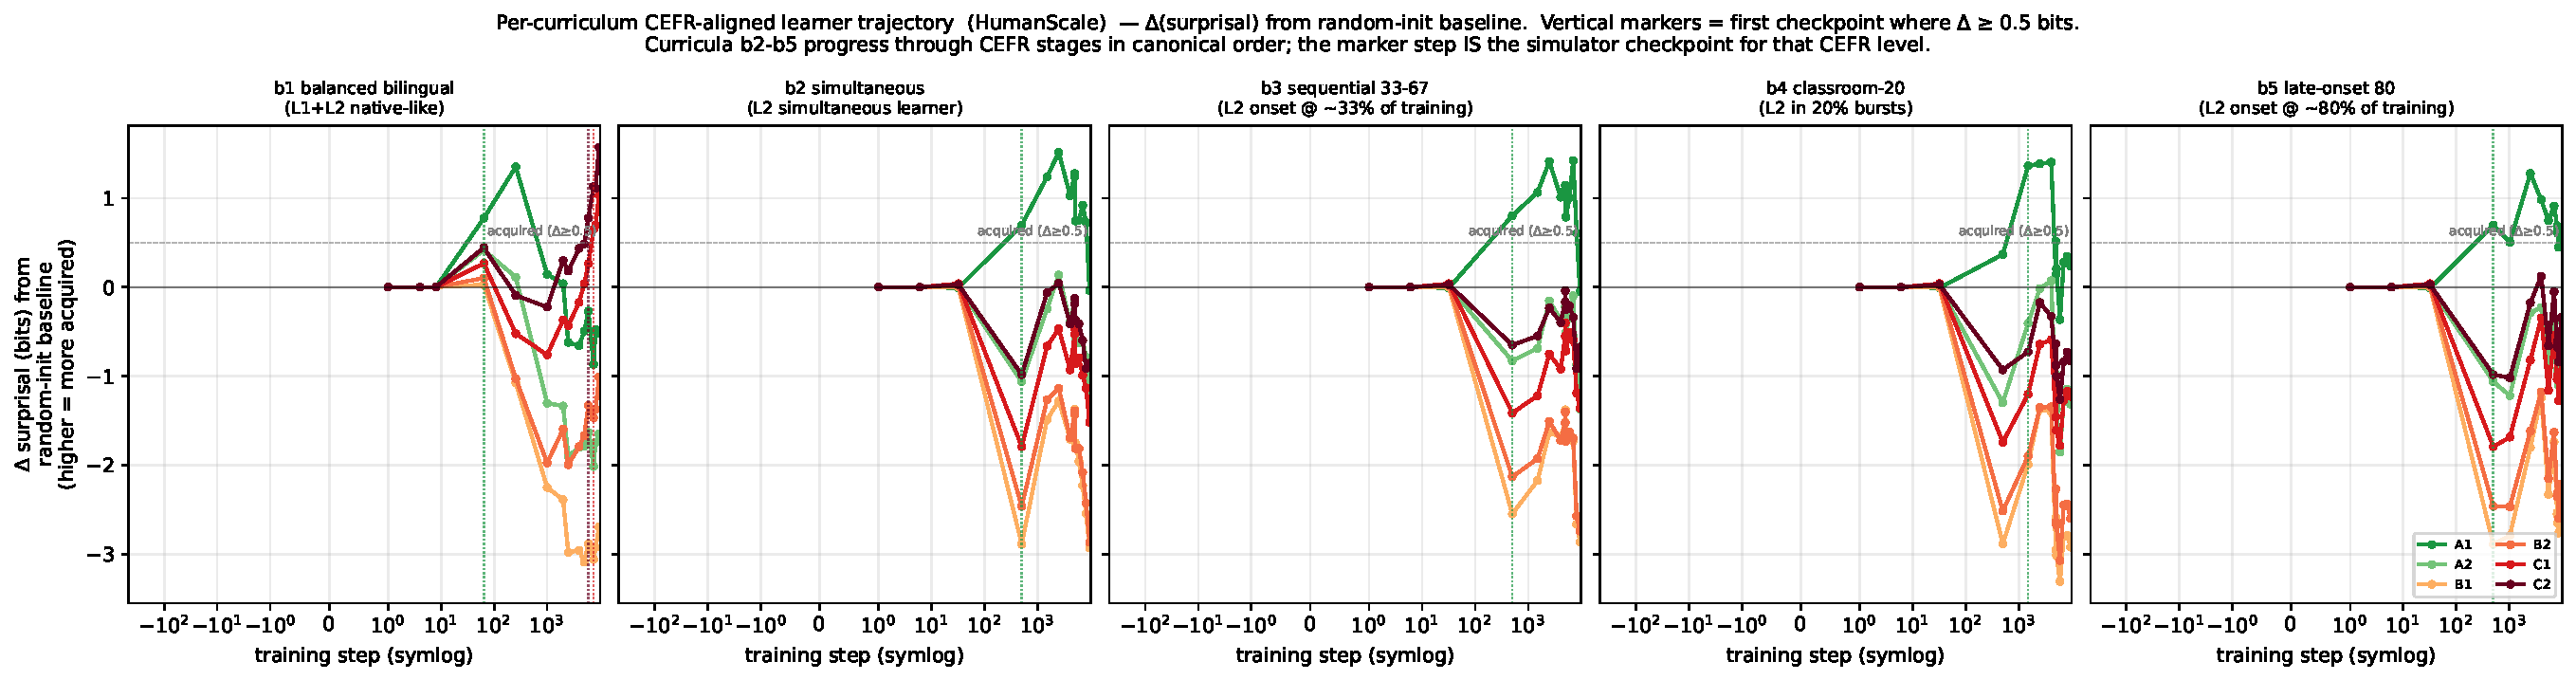
\includegraphics[width=0.86\linewidth,height=0.78\textheight,keepaspectratio]{fig/trajectory_cefr_humanscale.pdf}
  \caption{CEFR alignment trajectory at the \textsc{HumanScale}~100M token budget for \textsc{Beetle} curricula.}
  \label{appcomp:trajectory_cefr_humanscale}
\end{figure}

\newpage
\section{Supplementary Empirical Results}\label{sec:supp-results}

This section consolidates supplementary empirical content not folded into A.7--A.13: the continual-learning-overlay strategy comparison, the trilingual catastrophic-forgetting baseline, and the bilingual / trilingual learning-dynamics traces. See Tab.~\ref{tab:strategy_results} for the headline overlay-vs-base table; the layer-wise reading-time encoder profiles (Figs.~\ref{fig:D8_layerwise_profile}, \ref{fig:D9_peak_layer}) and representational-similarity diagnostics (Fig.~\ref{fig:repsim_b1_vs_b3}) live earlier in the appendix under A.7.

\subsection{Continual-learning overlay comparison}

\begin{figure*}[!ht]
    \centering
    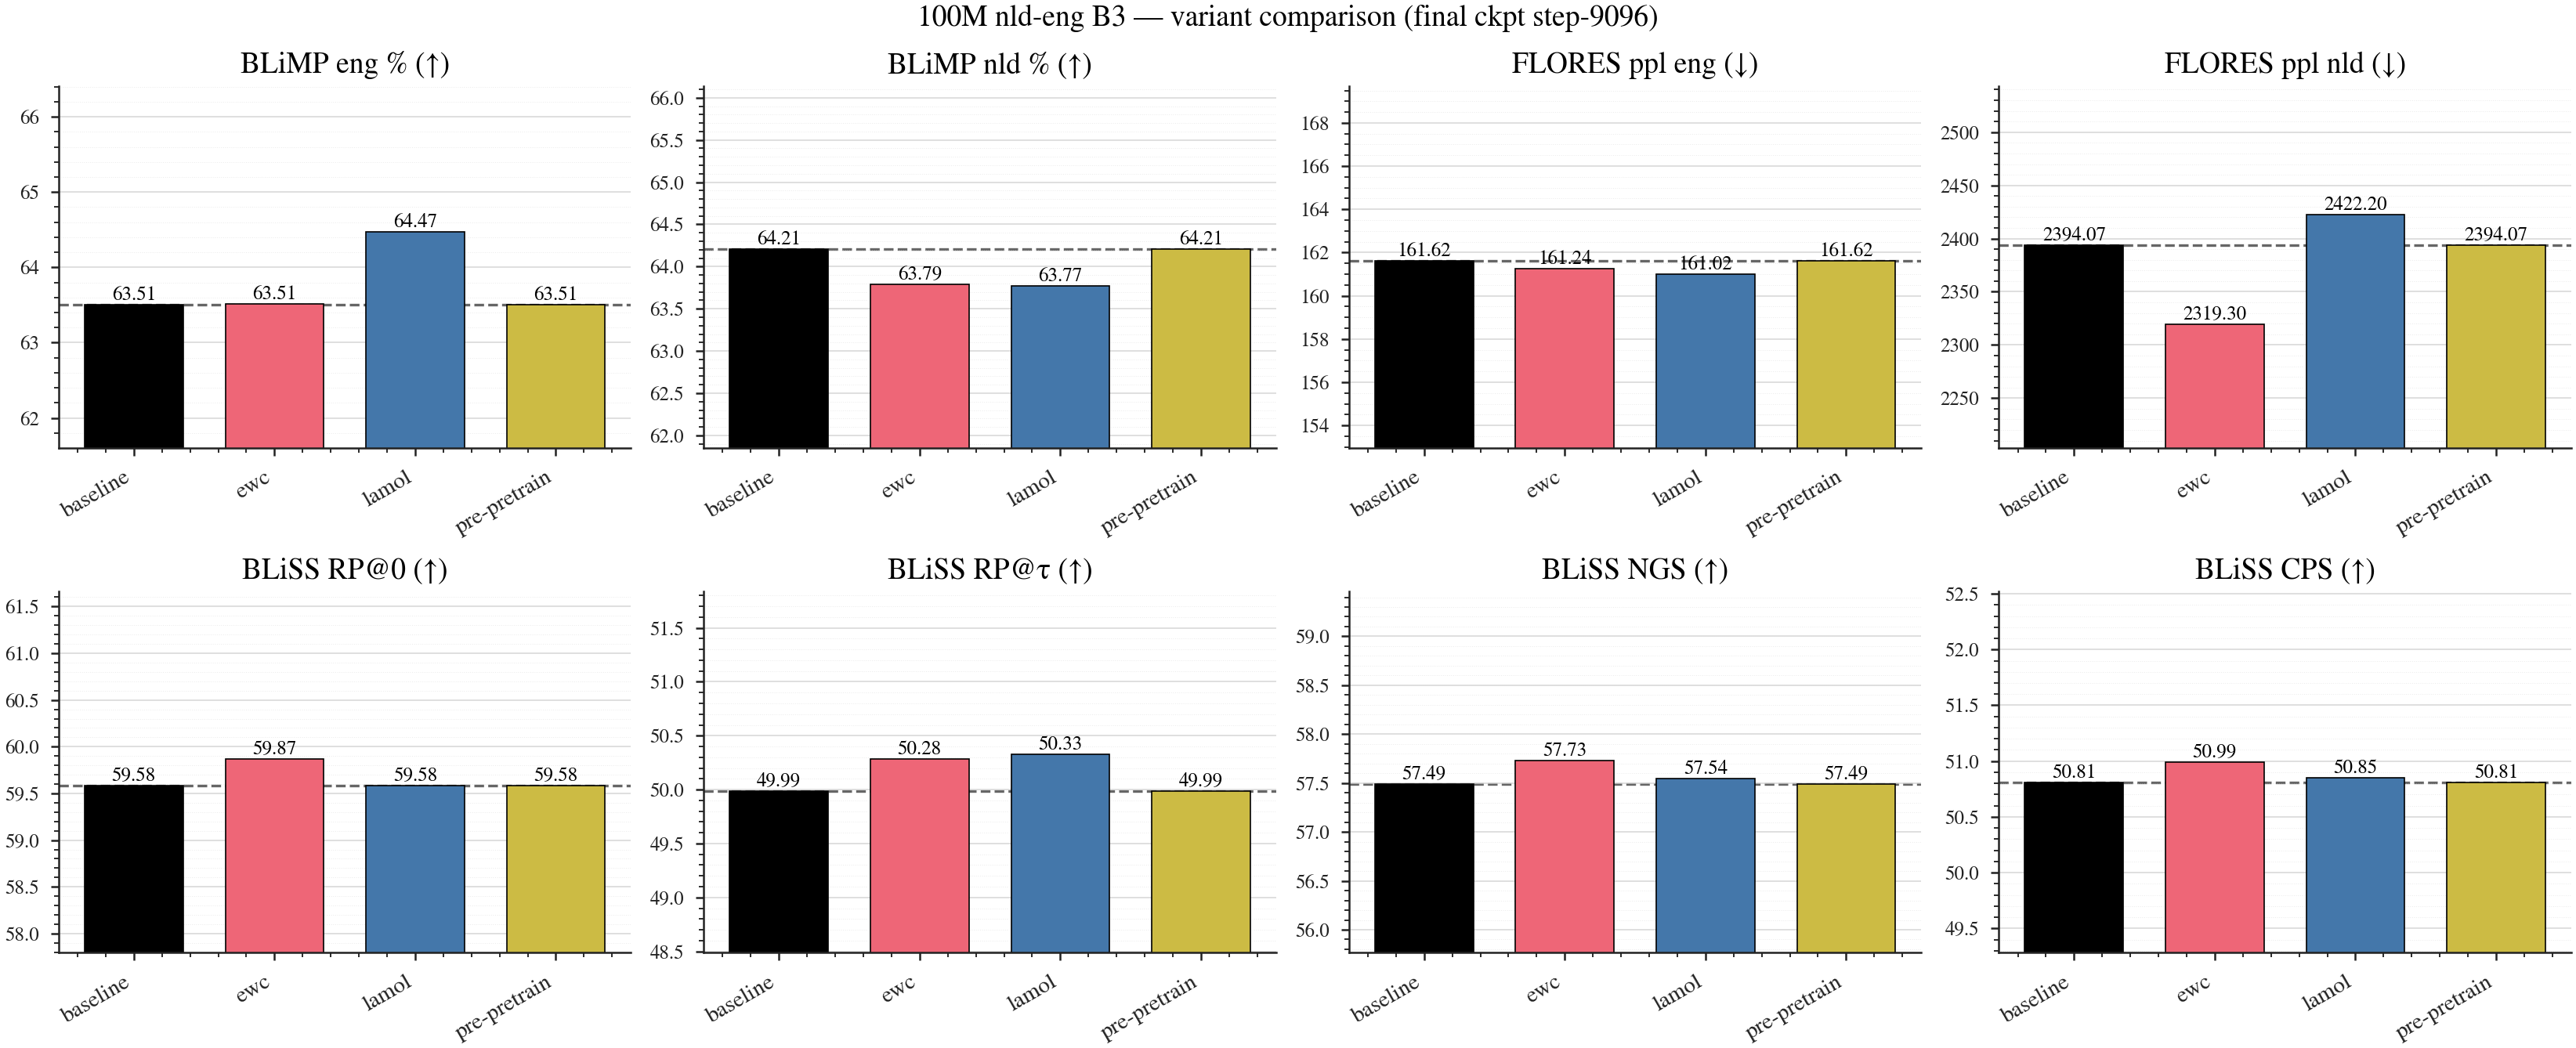
\includegraphics[width=0.86\linewidth,height=0.78\textheight,keepaspectratio]{fig/fig_variant_comparison_100m.png}
    \caption{\textbf{Continual-learning overlay comparison at HumanScale 100M.} BLiMP-eng, BLiMP-nl, BLiSS RP@0 / RP@$\tau$ / NGS / CPS, and MECO~L2 alignment for the five overlay variants (base, EWC, LAMOL, pre-pretrain, ALiBi) on the matched nld--eng \textsc{HumanScale} cohort. Companion to Tab.~\ref{tab:strategy_results}; overlay effects sit within $\pm 1.5$~pp of the base run across every axis.}
    \label{fig:cl_variant_comparison_100m}
\end{figure*}

\section{Roadmap and Planned Extensions}\label{sec:roadmap}

The released \beetle{} framework is configured to address seven planned extensions referenced from the body. Each item identifies a scientific question, the additional cells it requires, and the comparator against which the result should be read. Implementation details (scripts, configs, manifests) are provided with the released artefacts; we describe items here at the level of \emph{what would be measured}, not how to run them.

\paragraph{Item 1: Closing the typological gradient.} The reported MECO~L2 cells cover Dutch, German, and Chinese; the curriculum-by-task pattern is predicted to attenuate monotonically as the L1 moves further from English. Closure requires populating the five remaining L1 cells (Spanish, Russian, Finnish, Turkish, Hebrew) in the B1--B5 grid at \textsc{HumanScale} and at \textsc{FineWeb-2B}, against the same matched monolingual-anchor and BLOOM-560m parameter-matched controls used for the released L1s. The scientific reading is whether typological distance attenuates the curriculum advantage smoothly or in stepwise fashion at script and morphology boundaries.

\paragraph{Item 2: Chinese~L2 closure.} BLOOM-1b1 leads \beetle{} on the Chinese-reader MECO cell (164.3 vs.\ 115.4 $\Delta\log L$). Three confounded factors are observationally separable: (i) a typological-distance ceiling for 125M models; (ii) under-training of the zho--eng FineWeb cell relative to the Germanic cells; (iii) BLOOM's ROOTS pretraining mix containing a substantial Mandarin tail absent from the \beetle{} corpus. Closure requires extending the zho--eng cell to a matched 24~B-token budget and re-evaluating BLOOM-1b1 under our pipeline, alongside the Item~1 matched control to remove the data-composition confound.

\paragraph{Item 3: Reverse-direction sweeps.} All reported cells are forward-direction (non-English L1~$\to$~English~L2); the reverse cohort (English~L1~$\to$~non-English~L2) probes a distinct transfer question that we do not collapse with the forward direction in any figure. A reverse-direction \textsc{FineWeb-2B} sweep matched to the forward grid is the minimal extension; it relies on the bilingual L2 reading-time and CEFR resources for non-English targets, which are currently absent for several L1s.

\paragraph{Item 4: RACE-SFT pedagogical-utility ladder.} The body identifies a parameter-scale ceiling on RC-MCQ at 125M (\S\ref{sec:discrim-cefr}). A CEFR-stratified supervised fine-tune on RACE \citep{lai-etal-2017-race} of the B2 / B3-33 FineWeb-2B checkpoints would close the gap to the GPT-3.5 / GPT-4o-mini reference rows of \citet{benedetto-etal-2024-using}, and would let the pedagogical-utility ladder of Fig.~\ref{fig:ped_ladder} be read against the body's zero-shot bar rather than as a placeholder.

\paragraph{Item 5: Seed-grid extension.} Headline MECO~L2 and BLiSS cells are single-seed; the pre-registered seed grid $\{13, 42, 97\}$ on the nld--eng B1--B3 family (Tab.~\ref{tab:ablation-sweep}) is the minimal replication. Widening it to the full released-L1 $\times$ B1--B5 matrix at \textsc{HumanScale} yields between-seed standard deviations and turns the within-top-3 metric-dependent reordering (\S\ref{sec:pareto}) from a single-seed observation into a tested claim. We expect within-\beetle{} curriculum-family differences to be more seed-sensitive than the BLOOM-vs-\beetle{} headline gap, which on the matched Dutch-reader cell exceeds 100~$\Delta\log L$. \emph{In flight.} The base-condition slice of this extension --- the nld--eng B1 / B2 / B3-33 cells under the same $\{13, 42, 97\}$ seed grid, run on the \textsc{HumanScale} 100~M pipeline --- is now training (driver: \texttt{beetlelm/script/seedgrid\_b1\_b2\_b3\_nld\_eng.sh}; eval hook: \texttt{beetle-analyze/scripts/eval\_seedgrid\_b1\_b2\_b3\_nld\_eng.sh}; plan: \texttt{plan/seed\_grid\_b1\_b2\_b3\_nld\_eng\_plan.md}). The output is the per-cell $\Delta\log L$ between-seed standard deviation on B1 / B2 / B3-33, which converts the matched Dutch-reader B2-vs-B3-33 reordering from a single-seed observation to a tested claim and replaces the single-seed flag on the German-reader B3-33 nld--eng HS cell of Tab.~\ref{tab:meco_full_canonical} (footnote $^\dagger$).

\paragraph{Item 6: Bilingual induction-head emergence window.} A bilingual analogue to the monolingual $\sim$2\,B-token tipping point of \citet{aoyama-wilcox-2025-language} predicts that structured-exposure curricula shift the induction-head emergence window earlier in training. Measurement requires running the induction-head metric of \citet{aoyama2025predicting} on the log-spaced \beetle{} checkpoints between $2^{8}$ and $2^{18}$ steps, then taking the per-curriculum median onset across the released L1s. The release ships the analysis pipeline alongside the checkpoints; the empirical window is the natural next reading.

\paragraph{Item 7: Polyglot ($N{>}3$) regime.} The framework parameterises N-way polyglot regimes (App.~\ref{sec:beetle-curricula}); trilingual schedules T1--T4 ship as configurations with the framework but evaluation results are not in this paper. The natural extension is a controlled three-way and four-way set on Germanic-plus-non-Germanic mixes that distinguishes additive-interference from typological-mediated transfer; this requires the additional reading-time and CEFR resources flagged in Item~3.
